% arara: pdflatex
% arara: pdflatex
% arara: pdflatex

% options:
% thesis=B bachelor's thesis
% thesis=M master's thesis
% czech thesis in Czech language
% slovak thesis in Slovak language
% english thesis in English language
% hidelinks remove colour boxes around hyperlinks

\documentclass[thesis=M,czech]{FITthesis}[2019/12/23]

\usepackage[utf8]{inputenc} % LaTeX source encoded as UTF-8

% \usepackage{amsmath} %advanced maths
% \usepackage{amssymb} %additional math symbols

\usepackage{dirtree} %directory tree visualisation

% % list of acronyms
% \usepackage[acronym,nonumberlist,toc,numberedsection=autolabel]{glossaries}
% \iflanguage{czech}{\renewcommand*{\acronymname}{Seznam pou{\v z}it{\' y}ch zkratek}}{}
% \makeglossaries

\usepackage{gensymb} %symbol stupne
\usepackage{todonotes}

\newcommand{\tg}{\mathop{\mathrm{tg}}} %cesky tangens
\newcommand{\cotg}{\mathop{\mathrm{cotg}}} %cesky cotangens

% % % % % % % % % % % % % % % % % % % % % % % % % % % % % % 
% ODTUD DAL VSE ZMENTE
% % % % % % % % % % % % % % % % % % % % % % % % % % % % % % 

\department{Katedra softwarového inženýrství}
\title{Engine pro renderování a procedurální generování voxelových světů}
\authorGN{Lukáš} %(křestní) jméno (jména) autora
\authorFN{Hepner} %příjmení autora
\authorWithDegrees{Bc. Lukáš Hepner} %jméno autora včetně současných akademických titulů
\author{Lukáš Hepner} %jméno autora bez akademických titulů
\supervisor{Ing. Adam Vesecký}
\acknowledgements{Doplňte, máte-li komu a za co děkovat. V~opačném případě úplně odstraňte tento příkaz.}
\abstractCS{V~několika větách shrňte obsah a přínos této práce v~češtině. Po přečtení abstraktu by se čtenář měl mít čtenář dost informací pro rozhodnutí, zda chce Vaši práci číst.}
\abstractEN{Sem doplňte ekvivalent abstraktu Vaší práce v~angličtině.}
\placeForDeclarationOfAuthenticity{V~Praze}
\declarationOfAuthenticityOption{4} %volba Prohlášení (číslo 1-6)
\keywordsCS{Nahraďte seznamem klíčových slov v češtině oddělených čárkou.}
\keywordsEN{Nahraďte seznamem klíčových slov v angličtině oddělených čárkou.}
% \website{http://site.example/thesis} %volitelná URL práce, objeví se v tiráži - úplně odstraňte, nemáte-li URL práce

\begin{document}

% \newacronym{CVUT}{{\v C}VUT}{{\v C}esk{\' e} vysok{\' e} u{\v c}en{\' i} technick{\' e} v Praze}
% \newacronym{FIT}{FIT}{Fakulta informa{\v c}n{\' i}ch technologi{\' i}}

\begin{introduction}
	%sem napište úvod Vaší práce
\end{introduction}

\chapter{Herní engine}
\todo{Historie herních enginů?}
Herní engine zajišťuje vykreslování scény a komunikaci s grafickou kartou, zpracování vstupu od uživatele, správu zdrojů. Poskytuje třídy s obecnou funkcionalitou, využívané generátorem terénu. Mezi ně patří:

\begin{itemize}
\item Práce s náhodnými jevy.
\item Načítání a generování L-systémů.
\item Továrna pro vytváření herních objektů.
\item Správa textur.
\end{itemize}

\section{Herní smyčka}
Moderní grafické programy nezpracovávají data dávkově, ale obvykle čekají na vstup od uživatele, který následně zpracují. Na rozdíl od většiny softwaru, hry běží i když uživatel neposkytuje žádný vstup. Hra nezamrzne, animace se vykreslují, monstra se pohybují po scéně. Klíčovou částí je neblokující zpracování vstupu~\cite{gpp_gl}.

\begin{verbatim}
while (true) {
  processInput();
  update();
  render();
}
\end{verbatim}

Základními kameny jsou zpracování vstupu, který se stal od posledního volání \texttt{processInput}. Funkce \texttt{update} posune herní simulaci o jeden krok. Volání \texttt{render} na závěr vše vykreslí na obrazovku. Zde vyvstává otázka, jak rychle herní smyčka běží.

\subsection{Variabilní časový krok}
Mějme dva hráče. První má výkonný počítač a hra běží rychlostí 60 FPS (snímků za vteřinu). Druhý hráč má méně výkonný počítač a hra běží rychlostí 6 FPS. Avatar druhého hráče by se pohyboval pouze desetinovou rychlostí. Rychlost hry je přímo závislá na rychlosti hardwaru.

Pokud nemáme kontrolu nad hardwarem, na kterém hra běží, je toto řešení nepřípustné. Implementace musí brát v potaz, jak dlouho trvá jedna iterace herní smyčky, a podle ní zvětšit nebo zmenšit krok o který bude simulace posunuta vpřed.

\begin{verbatim}
while (!game->Finished()) {
    const auto currentFrame = static_cast<float>(glfwGetTime());
    deltaTime = currentFrame - lastFrame;
    lastFrame = currentFrame;

    game->ProcessInput(deltaTime);
    game->Update(deltaTime);
    game->Render();
}
\end{verbatim}

Metodám měnícím herní stav je předána hodnota \texttt{deltaTime}. Vykreslení zachycuje stav scény v okamžiku zavolání, proto nezávisí na \texttt{deltaTime}.

\section{Vykreslení objektů}

Vykreslovací engine má za úkol převod scény definované v 3D prostoru, na 2D plochu zobrazovacího zařízení hráče. Tento proces začíná na CPU, kde jsou herní objekty převedeny na data (matice), která jsou poslána grafické kartě. Zde jsou za pomocí série kroků transformována na zobrazitelné pixely. Tyto kroky jsou vysoce specializované a výstup každého z nich je použit jako vstup pro další. 

Tyto kroky je možné masivně paralelizovat a využít tisíců jader, které může grafická karta obsahovat. Každé jádro spouští malý program, pro každý krok vykreslovacího řetězce. Tyto programy jsou nazývané shadery. Některé ze shaderů může definovat vývojář a nahradit nimi existující výchozí shadery. OpenGL pro jejich programování využívá OpenGL shading language (GLSL)~\cite{lopgl_triangle}.

\subsection{Předání dat grafické kartě}

Scéna je složena z kusů terénu (třída \texttt{Chunk}), obsahující herní objekty. Chunky jsou rozmístěné na ploše vymezené osami \texttt{x} a \texttt{z}. Třída \texttt{Scene} má za úkol správu chunků a serializaci jejich dat do 1D pole, předané grafické kartě.

Každý herní objekt lze reprezentovat jako matici 4x4 obsahující informace o posunu vůči počátku světa, škálování a textuře.

\todo{dopsat informace o model matrix}

Převod herního objektu na matici:

\begin{verbatim}
for (const auto& o : obs) {
    assert(o.HasComponent<Components::Transform>());
    auto model =
        o.GetComponent<Components::Transform>().ModelMat();

    assert(o.HasComponent<Components::SpritesheetTex>());
    const auto& texPos = 
        o.GetComponent<Components::SpritesheetTex>().GetTexPos();
    Helpers::Math::PackVecToMatrix(model, texPos);

    buffer[cube]->push_back(model);
}

[[nodiscard]] glm::mat4 ModelMat() const {
    auto model = glm::mat4(1.0f); // identity matrix
    model = glm::translate(model, Position);
    return glm::scale(model, Scale);
}
\end{verbatim}

\subsubsection{Instancing}

Herní scéna obsahuje velké množství objektů se stejnou geometrií (např. krychle), s různou transformací vůči počátku světa. Každá krychle je složena z 12 trojúhelníků. Její vykreslení je téměř okamžité. Pokud by pro každou z nich bylo voláno samostatné vykreslení (draw call), velice rychle doje k drastickému snížení výkonu (komunikace s kartou přes sběrnici, uložení dat do patřičných bufferů\dots). Lepší řešení je poslat všechna data kartě najednou a ty následně vykreslit pomocí stejné geometrie. Toto řešení se nazývá instancing~\cite{lopgl_instancing}.

Scéna umožňuje definovat vlastní geometrie -- krychle, krychle bez podstav, nebo jakákoliv jiná kombinace stěn krychle. Pro každou z nich alokuje místo na grafické kartě, uloží do něj data objektů a následně samostatně vykreslí každou z nich.

\begin{verbatim}
// bind data
glBindBuffer(GL_ARRAY_BUFFER, InstanceDataBufferIds_[cube]);
unsigned offset = 0;
for (const auto& chunk : instancesData) {
    glBufferSubData(
        GL_ARRAY_BUFFER,
        offset * sizeof(glm::mat4), 
        chunk->size() * sizeof(glm::mat4), 
        chunk->data());
    offset += chunk->size();
}

CubeRenderers_[cube].GetDefaultMesh().BindBatchAttribPtrs();
\end{verbatim}

Rozdílné geometrie jsou užitečné, pokud chceme definovat krychli s rozdílnými podstavami a stěnami. Na obrázku~\ref{fig:block_composition}, lze vidět blok trávy složený ze tří částí.

\begin{figure}\centering
	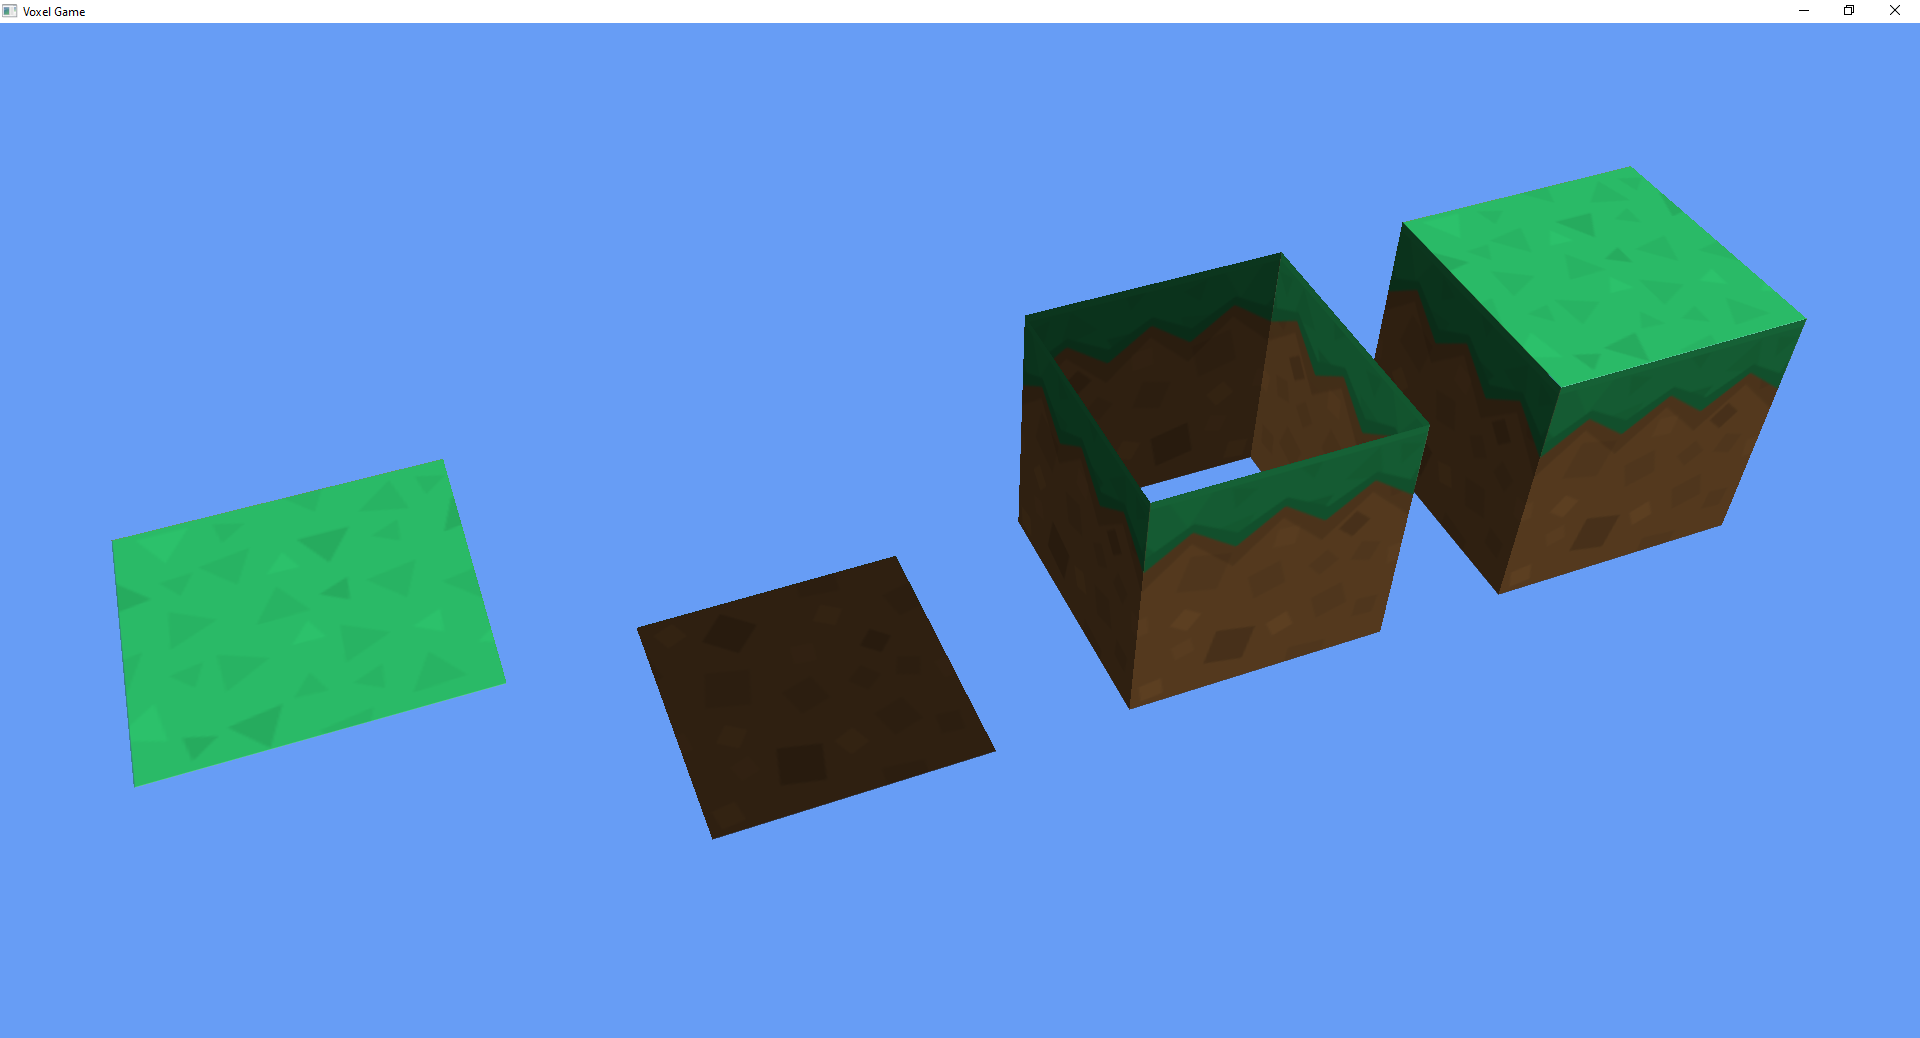
\includegraphics[width=\textwidth]{images/block_composition}
	\caption[Složení bloku ze tří částí]{Složení bloku ze tří částí}\label{fig:block_composition}
\end{figure}

\subsection{Společná data objektů}

Instancing umožňuje grafické kartě používat společná data pro všechny vykreslované objekty. Jeho protějškem v objektovém světe je návrhový vzor Flyweight.

Pokud má být objekt vykreslitelný musí obsahovat komponentu \texttt{Transform} (určující jeho pozici a velikost) a komponentu \texttt{Mesh} (představující geometrii objektu) -- obrázek~\ref{fig:go_components}.

\begin{figure}\centering
	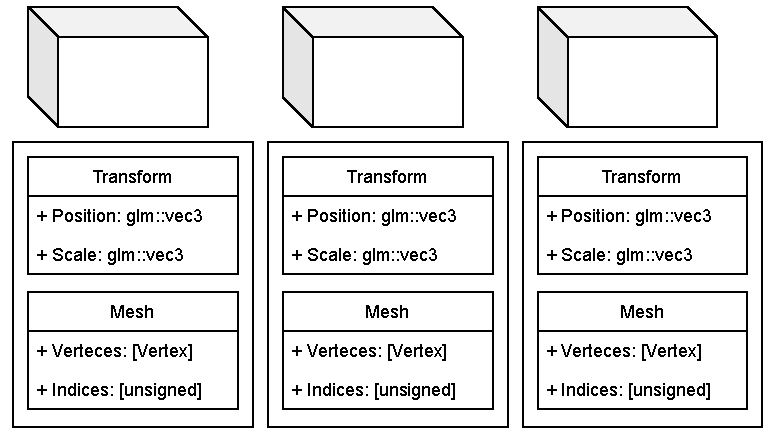
\includegraphics[width=\textwidth]{images/go_components}
	\caption[Komponenty herního objektu]{Komponenty herního objektu}\label{fig:go_components}
\end{figure}

\texttt{Mesh} obsahuje informace o vrcholech (\texttt{Vertex}) vykreslovaných trojúhelníků -- pozici na scéně, normálový vektor k úsečce mezi dvěma vrcholy trojúhelníku, pozici na textuře. A pole indexů, které říká, z jakých vrcholů jsou trojúhelníky složeny. Každý vrchol v má velikost $8 * 4 = 32$ B a \texttt{Mesh} jich obsahuje $6 * 4$. Každá stěna krychle má čtyři různé vrcholy\footnote{Krychle má 8 vrcholů. Vrcholy jednotlivých stěn se ale liší v normálovém vektoru a pozicí na textuře.}. Pole indexů má velikost $12 * 3 * 4$~B (počet trojúhelníků, počet vrcholů trojúhelníku, velikost \texttt{unsigned}). Celková velikost \texttt{Mesh}e představující krychli je:

\[8 * 4 * 6 * 4 + 12 * 3 * 4 = 912\; B\]

Pokud má být engine schopný vykreslovat desetitisíce objektů je tato paměťová náročnost neúnosná. Komponentu \texttt{Mesh} není možné odebrat z herního objektu, protože obsahuje pozici na textuře, lišící se mezi objekty. Pozice na textuře představuje čtverec, který bude vybrán z textury a aplikován na povrch krychle. Všechny objekty mají texturu čtverce. Díky tomu je možné definovat čtverec na počátku textury a jeho posun uložit do samostatné komponenty -- \texttt{SpritesheetTex}. Toto nové rozložení je znázorněno na obrázku~\ref{fig:go_components_fw}.

\begin{figure}\centering
	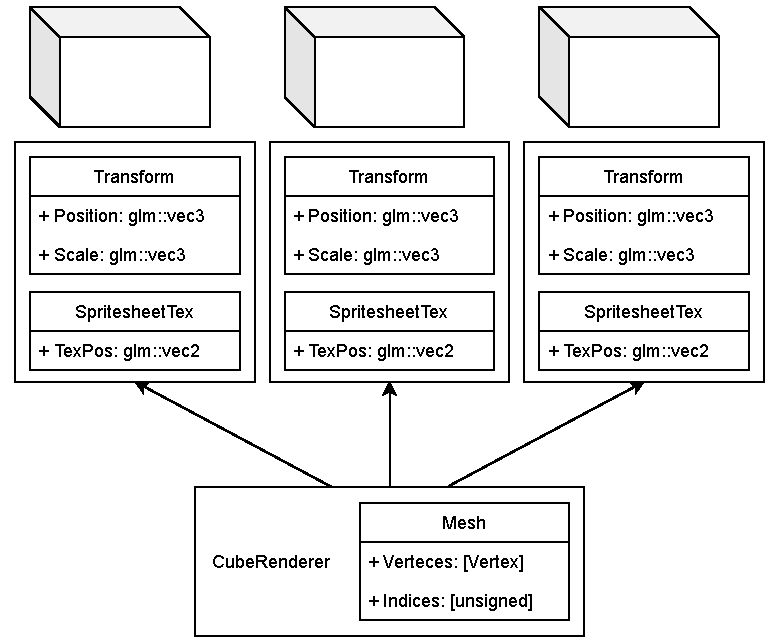
\includegraphics[width=\textwidth]{images/go_components_fw_2}
	\caption[Použití vzoru Flyweight]{Použití vzoru Flyweight}\label{fig:go_components_fw}
\end{figure}

Komponenta \texttt{SpritesheetTex} obsahuje dvě čísla ve formátu float (\texttt{float} je zvolen pro jednodušší komunikaci s grafickou kartou –- všechna předaná data mají formát float). Komponenta v paměti zabírá pouhých 8 B. Velikost herního byla redukována o 904 B.

\texttt{Mesh} není dále používána jako komponenta herního objektu. Její implementace ze jmenného prostoru \texttt{Renderer}, kterou komponenta \texttt{Mesh} obsahuje jako svůj atribut, je použita pro vykreslení všech objektů se stejnou geometrií najednou. Vykreslení objektů zajišťuje třída \texttt{CubeRenderer}, viz obrázek~\ref{fig:go_components_fw}.

% % % % % % % % % % % % % % % % % % % % % % % % % % % % 
% % Zpracování vstupu
% % % % % % % % % % % % % % % % % % % % % % % % % % % % 

\section{Zpracování vstupu}

O vstup z klávesnice a myši se stará abstraktní třída \texttt{InputHandler}, obsahující pole příkazů (třída \texttt{Command}) ovládajících kameru. Konkrétní implementaci má na starosti třída \texttt{InputHandlerGl}, pevně svázaná s voláními OpenGL.

Vstup je zpracován dvojím způsobem:

\begin{enumerate}
\item \texttt{ProcessInput}, voláno v rámci herní smyčky.
\item Zpětné volání z OpenGL.
\end{enumerate}

Pohyb hráče zajišťuje metoda \texttt{ProcessInput}. Délka pohybu je škálována parametrem \texttt{delta}. Vstupy jsou zpracovány při volání metody, kontrolou kláves, které jsou právě stlačené. Tento způsob je ideální pro kontinuální změnu stavu (např. pozice) objektu. Hráč může klávesu držet pro plynulý pohyb, nebo ji opakovaně mačkat pro drobné korekce.

Tento způsob je naprosto nevhodný pro změnu stavu nabývajícího několika diskrétních hodnot. Například vypnutí/zapnutí světla. Hráč musí klávesu stisknout a~pustit po dobu trvání jednoho snímku –- při 60~FPS na 16,67~ms. Při běžném stisknutí může dojít k několikanásobné změně stavu.

\subsection{Zpětné volání z OpenGL}

K zamezení opakovaného čtení stisknuté klávesy lze využít nastavení funkce, kterou OpenGL zavolá při stisknutí klávesy. Signatura této funkce musí být~\cite{glfw_callback}:

\begin{verbatim}
void function_name(
    GLFWwindow* window,
    int key, 
    int scancode, 
    int action, 
    int mods
)
\end{verbatim}

Výhody třídní hierarchie (dědění z obecné třídy pro zpracování vstupu a její konkrétní implementace pro OpenGL, možnost mít více objektů kontrolujících vstup a jejich výměna pro změnu ovládaní) znemožňují nastavení přímého volání metody z OpenGL -- metoda je závislá na stavu objektu, pro použití jako zpětné volání by musela být statická. Zpětné volání zajišťují funkce umístěné ve~jmenném prostoru \texttt{Input::Detail}.

\begin{verbatim}
namespace Input::Detail {
void CursorPosCallback(GLFWwindow*, double xPos, double yPos) {
    currentHandler->ProcessMouse(
        static_cast<float>(xPos),
        static_cast<float>(yPos));
}

void ScrollCallback(GLFWwindow*, double, double yOffset) {
    currentHandler->ProcessMouseScroll(
        static_cast<float>(yOffset));
}

void KeyCallback(GLFWwindow*, int key, 
                 int scanCode, int action, int mods) {
    currentHandler->ProcessKey(key, scanCode, action, mods);
}
} // namespace Input::Detail
\end{verbatim}

Tyto funkce nejsou umístěné v hlavičkovém souboru a uživatel by je neměl napřímo využívat.  Zpětné volání je automaticky nastaveno při inicializaci objektu.

\begin{verbatim}
void Input::InputHandlerGl::SetCallBacks()
{
Detail::currentHandler = this;
WindowManagerGl::SetCursorPosCallback(Detail::CursorPosCallback);
WindowManagerGl::SetScrollCallback(Detail::ScrollCallback);
WindowManagerGl::SetKeyCallback(Detail::KeyCallback);
}
\end{verbatim}

Jmenný prostor \texttt{Input::Detail} obsahuje pouze jednu proměnnou, označující současný objekt zpracovávající vstup.

\subsection{Návrhový vzor příkaz}
Jednoduchá implementace kódu zpracovávajícího vstup by mohla vypadat:

\begin{verbatim}
void InputHandler::handleInput() {
    if (isPressed(BUTTON_W)) object.MoveForward();
    else if (isPressed(BUTTON_S)) object.MoveBackward();
    else if (isPressed(BUTTON_A)) object.MoveLeft();
    else if (isPressed(BUTTON_D)) object.MoveRight();
}
\end{verbatim}

Tento kód funguje, pokud jsme ochotni natvrdo zadrátovat vstup hráče k~herním akcím viz obrázek~\ref{fig:ih_old}, ale hodně her hráče nechá nakonfigurovat si vlastní mapování tlačítek. K tomuto potřebujeme vyměnit přímé volání metody A za metodu B. K tomu potřebujeme objekt reprezentující volání metody~\cite{gpp_cmd}.

\begin{figure}\centering
	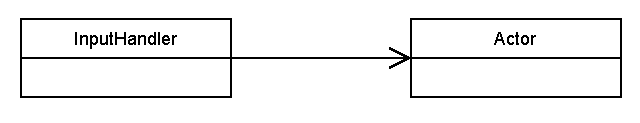
\includegraphics[width=\textwidth]{images/ih_old}
	\caption[Přímé propojení InputHandler s Actor]{Přímé propojení InputHandler s Actor}\label{fig:ih_old}
\end{figure}

Definujme abstraktní třídu \texttt{Command} představující spustitelný příkaz.

\begin{verbatim}
class Command {
  protected:
    Renderer::Camera* Actor;

  public:
    explicit Command(Renderer::Camera* actor) : Actor(actor) {}
    virtual ~Command() = default;

    virtual void Execute(float delta) = 0;
};
\end{verbatim}

V konkrétní implementaci příkazu je z něj poděděno a metoda \texttt{Execute} přepsána pro specifické chování.

\begin{verbatim}
class MoveForwardCommand : public Command {
  public:
    explicit MoveForwardCommand(Renderer::Camera* actor) 
        : Command(actor) {}
    void Execute(float delta) override {
        Actor->Move(delta, 0.0, 1.0);
	}
};
\end{verbatim}

\texttt{InputHandler} je odstíněn od volání prováděných na \texttt{actor} (obrázek~\ref{fig:ih_new}), sníží se tak spojení mezi třídami a zvýší se soudržnost (high cohesion). \texttt{InputHandler} má na starosti zpracování vstupu, ne ovládání herní postavy.

\begin{figure}\centering
	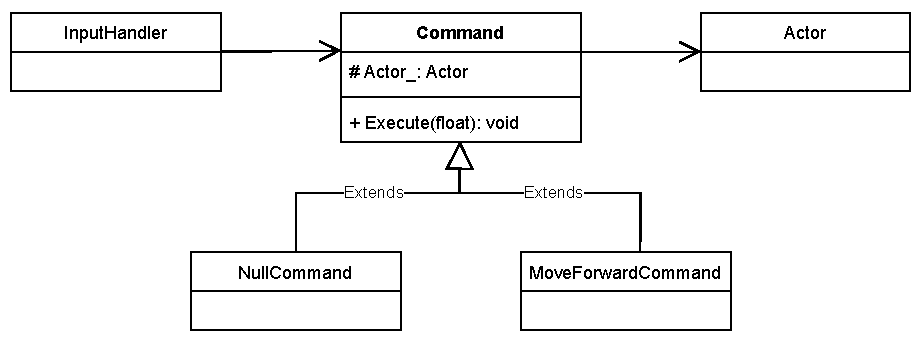
\includegraphics[width=\textwidth]{images/ih_new}
	\caption[Využití třídy Command]{Využití třídy Command}\label{fig:ih_new}
\end{figure}

Příkazy jsou uloženy v poli:
\begin{verbatim}
std::array<std::unique_ptr<Commands::Command>, Keys::Count> 
    Commands
\end{verbatim}
Toto pole je naplněno při inicializaci \texttt{InputHandler}u, neobsahuje tedy žádné \texttt{nullptr} ukazatele. Při odstranění příkazu reagujícího na stlačení tlačítka, by při jeho stisku došlo k vyhození \texttt{nullptr} výjimky a pádu programu. Toto chování může být ošetřeno důslednou kontrolou obsahu \texttt{unique\_ptr}, byl by tím ovšem porušen objektový návrh. Řešení použité v enginu je \texttt{NullCommand}.

\begin{verbatim}
class NullCommand : public Command {
  public:
    NullCommand() : NullCommand(nullptr) {}
    explicit NullCommand(Renderer::Camera*) :Command(nullptr){}
    void Execute(float) override {}
};
\end{verbatim}

Toto řešení zachovává principy objektového návrhu. Přijímá parametr \texttt{actor}, svému předku však předá \texttt{nullptr}. Tělo metody \texttt{Execute} je prázdné a s \texttt{actor}em není interagováno. Volání metody \texttt{Execute} mohou být bezpečně provedena na všech prvcích pole.

% % % % % % % % % % % % % % % % % % % % % % % % % % % % 
% % Modelování rostlin s využitím L-systémů
% % % % % % % % % % % % % % % % % % % % % % % % % % % % 

\chapter{Vykreslování scény}

OpenGL představuje stavový automat. Jeho výchozí hodnoty jsou nastaveny při spuštění programu (např.: způsob mísení barev, povolení testu hloubky\dots). Některé se musí měnit podle dat, které se mají vykreslit (např.: face culling). Grafická karta má před každým voláním pro vykreslení scény uložena data objektů ve svých bufferech. Přiřazené textury do texturovacích jednotek. Nastavené proměnné shaderů a shadery, které se mají pro vykreslení použít. Tyto parametry představují stav OpenGL, podle něhož se vykreslí scéna. Vykreslení může probíhat ve více krocích -- vykreslovací příkaz OpenGL je zavolán několikanásobně. Při každém volání proběhnou následující kroky~\cite{kronos_render}:

\begin{enumerate}
\item Specifikace vrcholů --- Načtení formátu vrcholů a předání dat, která budou zpracována dále v řetězci. 

\item Vertex shader --- Provede zpracování vrcholu na základě uživatelem specifikovaného programu a předá ho k dalšímu zpracování. Zpracován může být pouze jeden vrchol a ten musí být předán do dalšího kroku. Poskytnutí vertex shaderu je povinné.

\item Teselace --- Nepovinný krok, který může rozdělit primitivum (trojúhelník, úsečku\dots) na několik menších primitiv~\cite{kronos_tess}.

\item Geometry shader --- Uživatelem definovaný program, zpracovávající primitiva. Výstupem je nula nebo více primitiv. Vstupní a výstupní primitiva musí být přesně definovaná. Geometry shader může změnit jeho geometrii, provést transformaci souřadnic\dots Tento krok není povinný.

\item Post-processing vrcholů --- Složená primitiva (např.: pruh trojúhelníků) jsou převedena na jednoduchá primitiva (úsečky, body, trojúhelníky). Primitiva jejichž část se nachází mimo prostor obrazovky jsou rozdělena, aby vznikla nová, jež jsou uvnitř prostoru obrazovky. Trojúhelníková primitiva mohou být vyřazena, pokud nemíří k pozorovateli. Všechna nová primitiva jsou uložena do výstupních bufferů pro další zpracování.

\item Rasterizace --- Primitiva, která se dostanou do této fáze jsou převedena na fragmenty. Fragment je soubor hodnot obsahující výstupy předchozích shaderů. Jejich hodnota je nastavena interpolací hodnot vrcholů, z kterých se primitivum skládá. Každý fragment obsahuje pozici v~prostoru obrazovky~\cite{kronos_frag}.

\item Fragment shader --- Výstupem fragment shaderu je list barev, které budou zapsány do výstupních bufferů, hodnota hloubky a hodnota šablony (stencil value). Fragment shader může být definován uživatelem. Pokud není, hodnota barev není definovaná, je pouze zapsána hodnota hloubky a šablony.

\item Operace provedené na vzorcích (Per-Sample Operations) --- Výstupní data fragmentu jsou podrobena sérii testů (mohou být specifikované uživatelem, např.: hloubkový test), které je mohou vyřadit z podílení se na výsledné barvě pixelu. Pokud projdou, je provedeno míchání barev s barvami, které již obsahuje framebuffer.
\end{enumerate}

\todo{world coords, etc.}

\section{Vyřazení neviditelných částí objektu}

Část scény tvoří krychle mající všech šest stěn vyplněných neprůhlednou texturou. Při pohledu na krychli může hráč vidět maximálně tři její stěny najednou (z určitých úhlů pouze jednu nebo dvě). Minimálně 50~\% každé krychle je vykreslováno zbytečně. OpenGL je schopno vyřadit stěny, které směřují pryč od hráče, z vykreslovacího procesu a snížit počet volání fragment shaderu. Tato technika se nazývá face culling~\cite{lopgl_faceculling}.

K rozpoznání stěn (trojúhelníků), které směřují pryč od hráče OpenGL používá pořadí jeho vrcholů. Vrcholy mohou být definované ve směru nebo protisměru hodinových ručiček  -- obrázek~\ref{fig:winding_order}. Při pohledu na grafické primitivum z druhé strany, se změní pořadí jeho vrcholů. V~základním nastavení OpenGL, jsou primitiva s vrcholy definovanými po směru hodinových ručiček, považována za směřující k hráči.

\begin{figure}\centering
	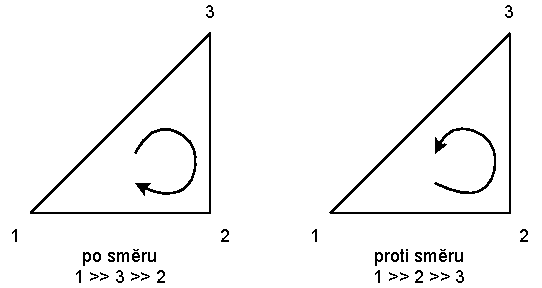
\includegraphics[width=\textwidth]{images/winding_order}
	\caption[Pořadí vrcholů]{Pořadí vrcholů}\label{fig:winding_order}
\end{figure}

Tato technika není v základním nastavení OpneGL zapnutá. Musí se povolit zavoláním funkce:

\begin{verbatim}
glEnable(GL_CULL_FACE);
\end{verbatim}

Pro objekty, které nemají všech šest stěn nebo mají průhlednou texturu, je nutné vypnou face culling. Hráči se zobrazí i vnitřek objektu, který by jinak nebyl vidět. Příkladem je vykreslování trávy -- obrázek~\ref{fig:face_culling}. Na pravém bloku je tráva vykreslena se zapnutým face cullingem. Na levém bloku je face culling vypnutý.

\begin{figure}\centering
	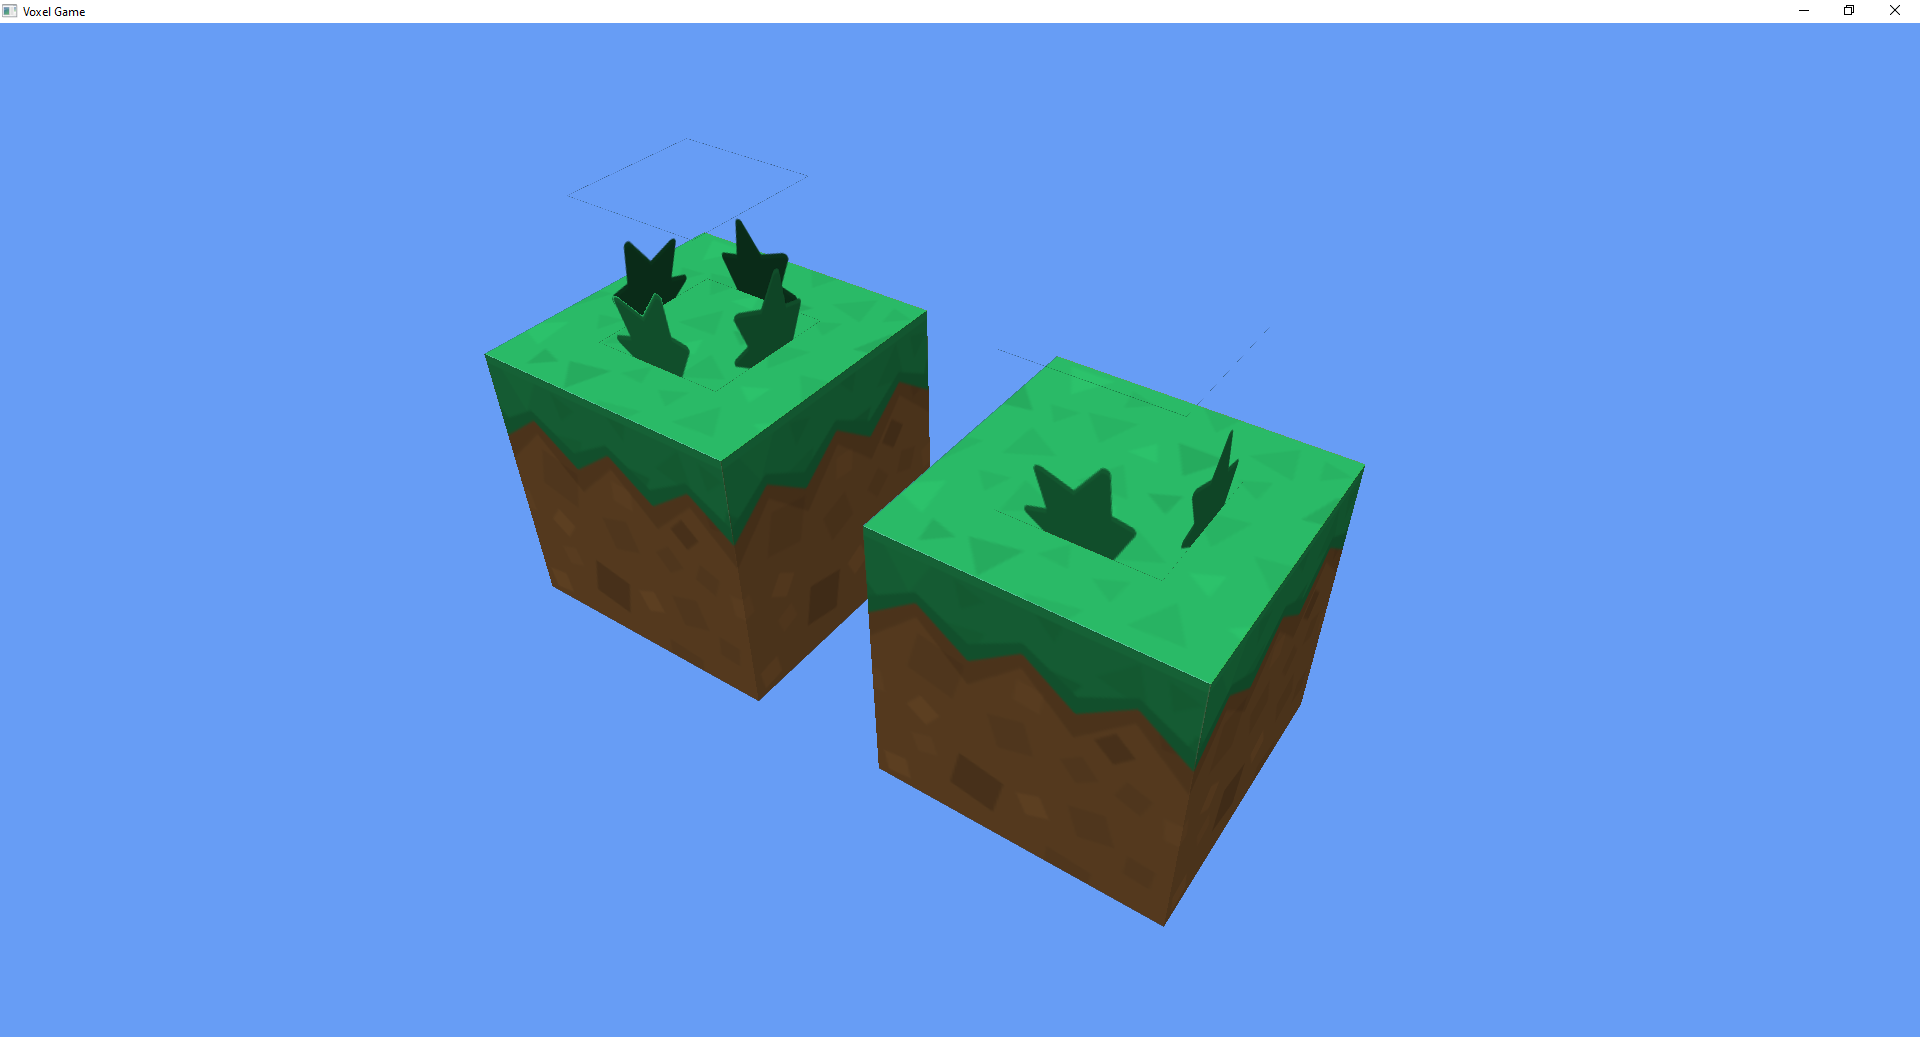
\includegraphics[width=\textwidth]{images/face_culling}
	\caption[Face culling]{Face culling}\label{fig:face_culling}
\end{figure}

\section{Průhledné a poloprůhledné textury}

Při vykreslování textur majících průhlednost (alfa $<$ 1) může nastat několik problémů. Prvním z nich je pořadí vykreslování objektů. Pokud má textura průhlednost, musí se její barva skombinovat s barvami textur, které překrývá. Na obrázku~\ref{fig:alpha} jsou textury vykreslovány postupně z pravého dolního rohu, po řádcích směrem k levému hornímu rohu. Lze si všimnou, že průhledná část trávy je korektně smíchána s~barvou bloku pod ní (je vykreslen první). Bloky v pozadí obrázku jsou překryté modrou barvou v~místech, kde je textura trávy průhledná.

\begin{figure}\centering
	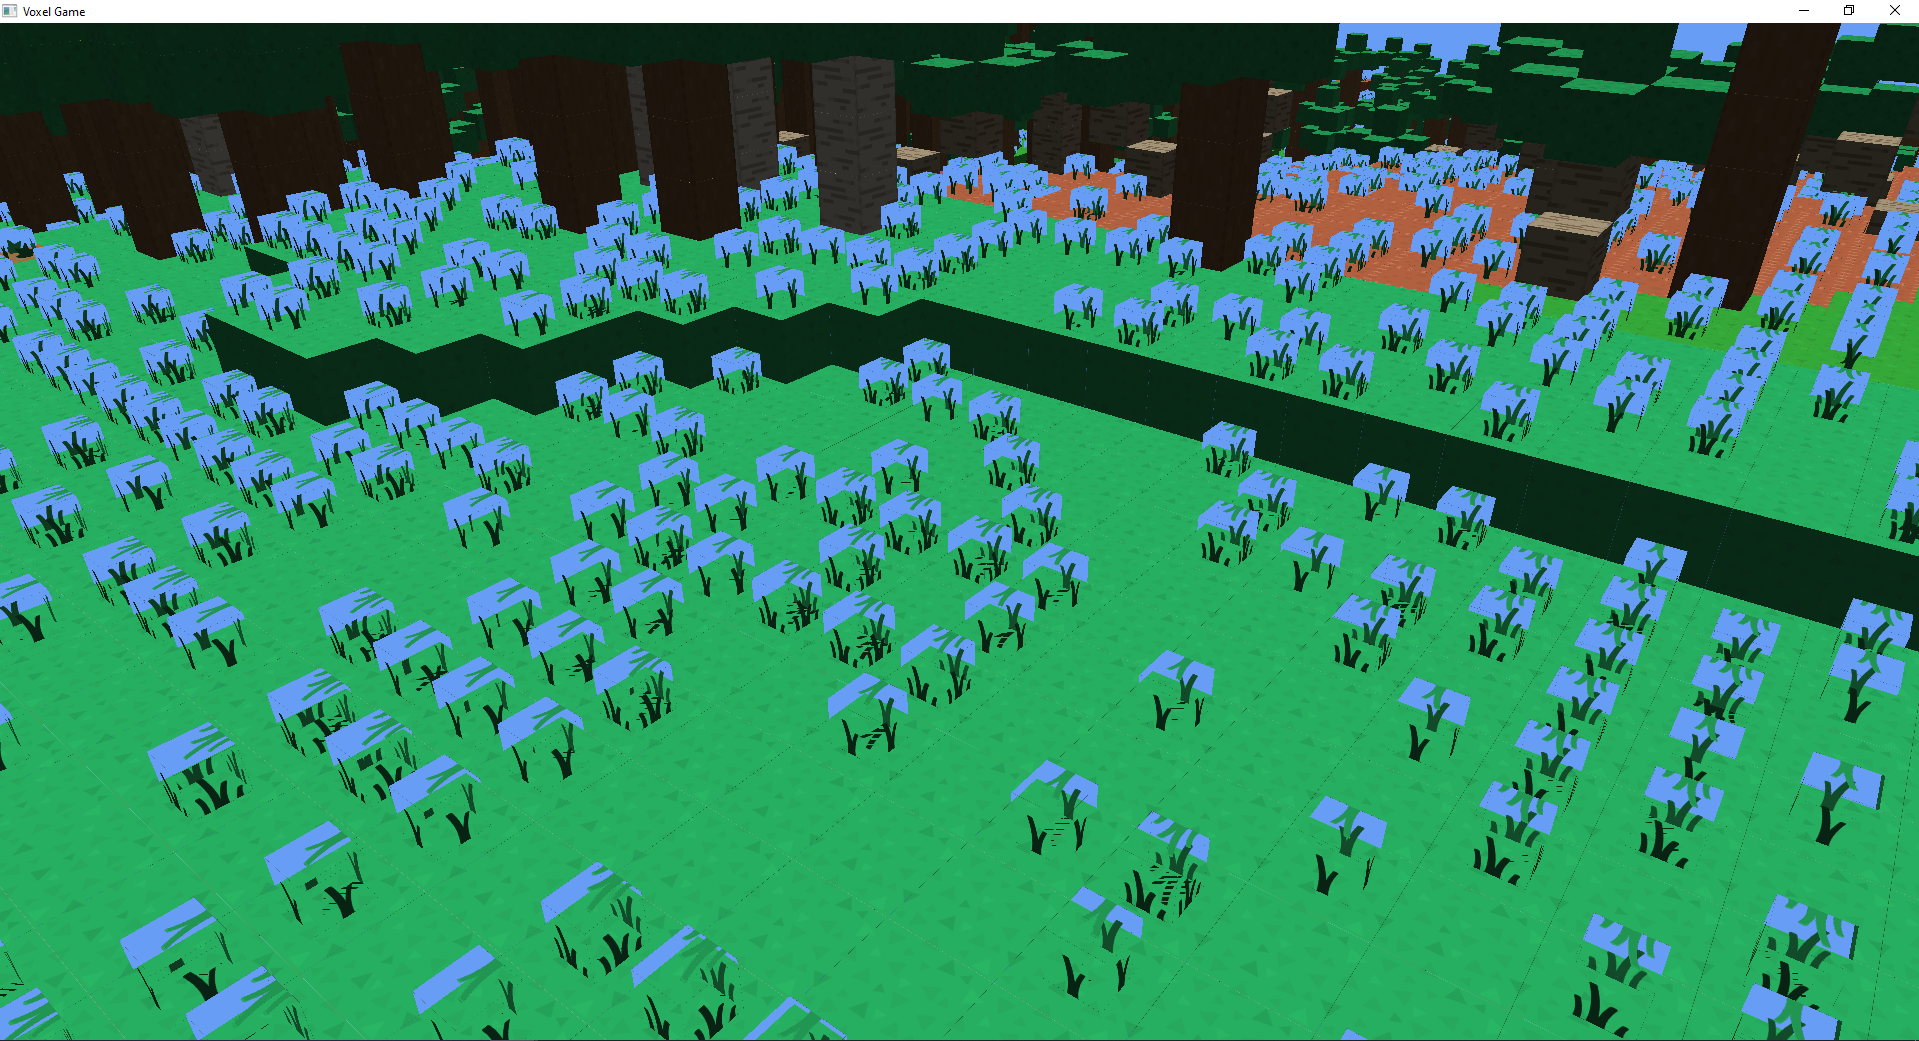
\includegraphics[width=\textwidth]{images/alpha}
	\caption[Prolínání průhledných částí textury s pozadím]{Prolínání průhledných částí textury s pozadím}\label{fig:alpha}
\end{figure}

Tento jev nastává kvůli použití depth bufferu, ten šetří výpočetní výkon zahozením fragmentů, které by nebyly vidět. Jsou do něj však uloženy všechny fragmenty nezávisle na průhlednosti. V ideálním případě by nejdříve měly být vykreslené všechny fragmenty, které se budou podílet na barvě pixelu, od nejvzdálenějšího k nejbližšímu~\cite{lopgl_blend}.

Toto řešení vyžaduje řazení objektů na scéně podle jejich vzdálenosti od kamery. Poloha kamery se s~pohybem hráče neustále mění a řazení objektů by snižovalo výkonost.

Avšak objekty bez průhledných části překryjí všechny objekty nehledě na průhlednost. Scénu tak lze rozdělit na dvě části. A objekty bez průhlednosti vykreslit jako první. Na obrázku~\ref{fig:alpha_cut_off} je tato technika implementována. Barva průhledné části trávy je korektně smíchána s barvou bloku v pozadí.

\begin{figure}\centering
	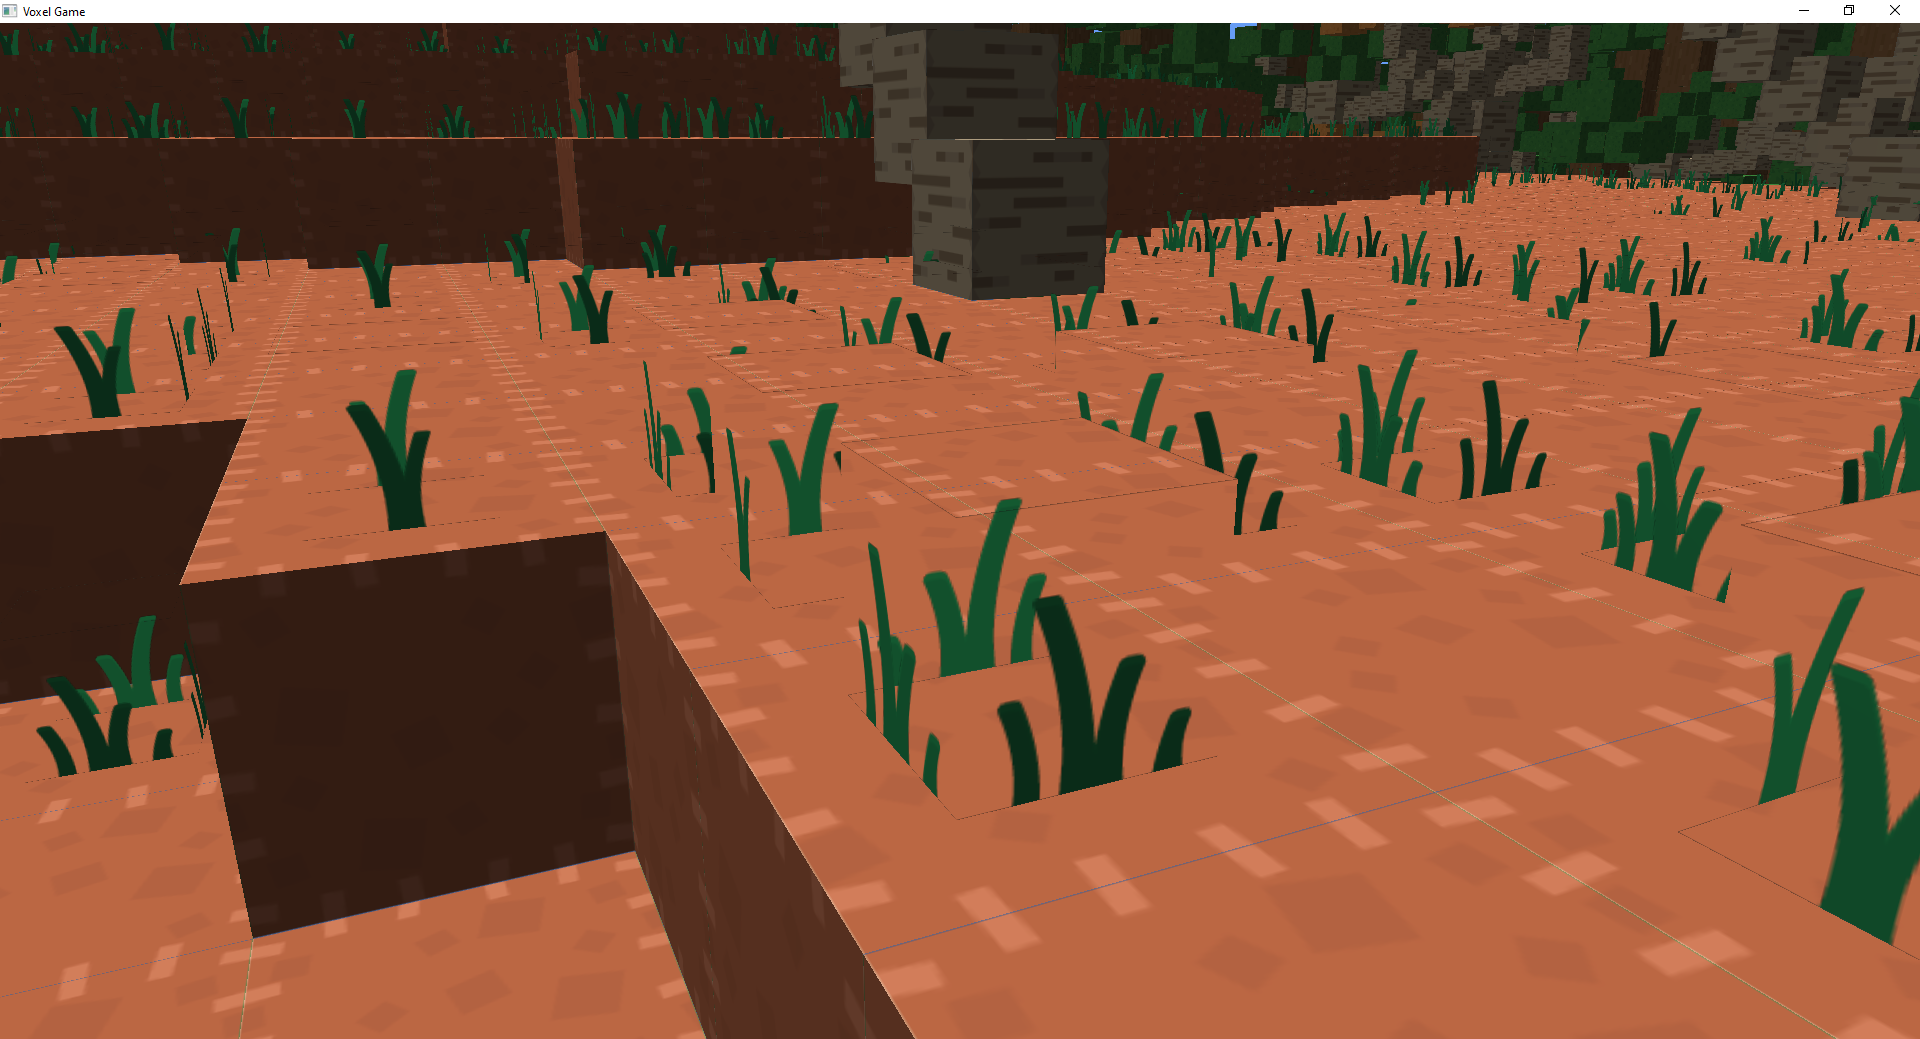
\includegraphics[width=\textwidth]{images/alpha_cut_off}
	\caption[Zastínění průhlednou částí textury]{Zastínění průhlednou částí textury}\label{fig:alpha_cut_off}
\end{figure}

Problém s pořadím textur obsahujících průhlednost stále přetrvává. Na obrázku~\ref{fig:alpha_cut_off} lze jasně vidět průhlednou část textury trávy, překrývající trávu v pozadí. Pro textury mající části úplně průhledné nebo úplně neprůhledné lze problém vyřešit ve fragment shaderu. Všechny framenty, mající průhlednost menší, než stanovená mez, budou vyřazeny z vykreslovacího řetězce.

\begin{verbatim}
float alpha = vec4(texture(texture_diffuse1, TexCoord)).a;
if (alpha < 0.05)
    discard;
\end{verbatim}

Problém s poloprůhlednými texturami však přetrvává a pro jeho vyřešení je nutné poloprůhledné textury seřadit.

\section{Osvětlení scény}

Osvětlení v reálném světě je extrémně složitý problém. Jeho přesná simulace v aplikacích reálného času je výpočetně náročná. Pro zjednodušení výpočtu existují modely, které produkují výsledky podobné reálnému světu.

\subsection{Phongův osvětlovací model}

Jednou z aproximací reálného světa je Phongův osvětlovací model, skládající se ze tří hlavních částí~\cite{lopgl_basic_light}.

\begin{itemize}
\item Okolní (ambient) světlo --- I za tmy jsou objekty nasvíceny světlem odraženým od ostatních objektů (měsíc) nebo vzdáleným zdrojem světla (hvězdy). Objekty většinou nejsou zcela tmavé. A nastavením konstanty pro ambientní osvětlení můžeme simulovat tento jev.

\item Difúzní světlo --- Simuluje dopad světla na objekt. Pokud je objekt natočen ke zdroji světla, bude ním více ovlivněn. 

\item Lesklé světlo --- Simuluje odraz světla od lesklého předmětu.
\end{itemize}

Výpočet osvětlení může být prováděn na CPU, nastavením světlosti každé stěny bloku. Pokud má být docíleno věrnějšího výsledku, je nutné počítat světlost pro každý fragment objektu (úhel dopadu světla se může výrazně lišit pro fragmenty na opačných stranách objektu). Výpočet je proto prováděn na grafické kartě, přesněji ve fragment shaderu.

Ambientní složka světla je předána grafické kartě, kde je vynásobena s barvou objektu -- textury.

\begin{verbatim}
vec3 ambient = 
    light.ambient * vec3(texture(texture_diffuse1, TexCoord));
\end{verbatim}

Pro výpočet difuzní složky, je shaderu předána pozice světla (\texttt{light.position}) a jeho barva (\texttt{light.diffuse}). Světlo dopadající kolmo na fragment má největší efekt na jeho výslednou barvu. Pro výpočet úhlu dopadu je využit normálový vektor fragmentu\footnote{Normálový vektor je předán vertex shaderu jako jeden z~atributů vrcholu trojúhelníku. Ten ho následně předá fragment shaderu.}. Vynásobením (skalární součin) normálového vektoru fragmentu a vektoru směřujícího od fragmentu ke světlu, je získána hodnota 1 pro vektory svírající nulový úhel a 0 pro kolmé vektory. Rozsah hodnot je zaručen normalizací vektorů.

Pokud vektory svírají úhel větší než 90° je hodnota skalárního součinu záporná. Tuto situaci si lze představit jako dopad světla z opačné strany fragmentu. Ten by tedy neměl být osvětlený, \texttt{diff} je nastaven na 0. Hodnota difuzní složky je vynásobena s barvou světla a fragmentu.

\begin{verbatim}
vec3 lightDir = normalize(light.position - FragPos);
float diff = max(dot(norm, lightDir), 0.0);
vec3 diffuse = diff * light.diffuse * 
    vec3(texture(texture_diffuse1, TexCoord));
\end{verbatim}

Intenzita odraženého světla (lesklá složka) je závislá na pozici pozorovatele (předána shaderu jako \texttt{view\_pos}). Pokud odražené světlo směřuje přímo do oka pozorovatele, je jeho intenzita nejvyšší. Vektor odraženého světla lze spočítat pomocí funkce \texttt{reflect}. Její první parametr je vektor směřující od světla k~fragmentu, tedy vektor opačný k \texttt{lightDir}. Druhý parametr je normálový vektor.

Intenzita je opět spočítána pomocí skalárního součinu, a umocněna lesklostí materiálu. Čím vyšší lesklost, tím méně je světlo rozptýleno do všech směrů a velikost efektu se zmenší~\cite{lopgl_basic_light}.

\begin{verbatim}
vec3 viewDir = normalize(view_pos - FragPos);
vec3 reflectDir = reflect(-lightDir, norm);
float spec = 
    pow(max(dot(viewDir, reflectDir), 0.0), material.shininess);
vec3 specular = spec * light.specular * 
    vec3(texture(texture_diffuse1, TexCoord));
\end{verbatim}

Na obrázku~\ref{fig:phong} je vykreslená bedna osvícena všemi druhy světel a jejich kombinací.

\begin{figure}\centering
	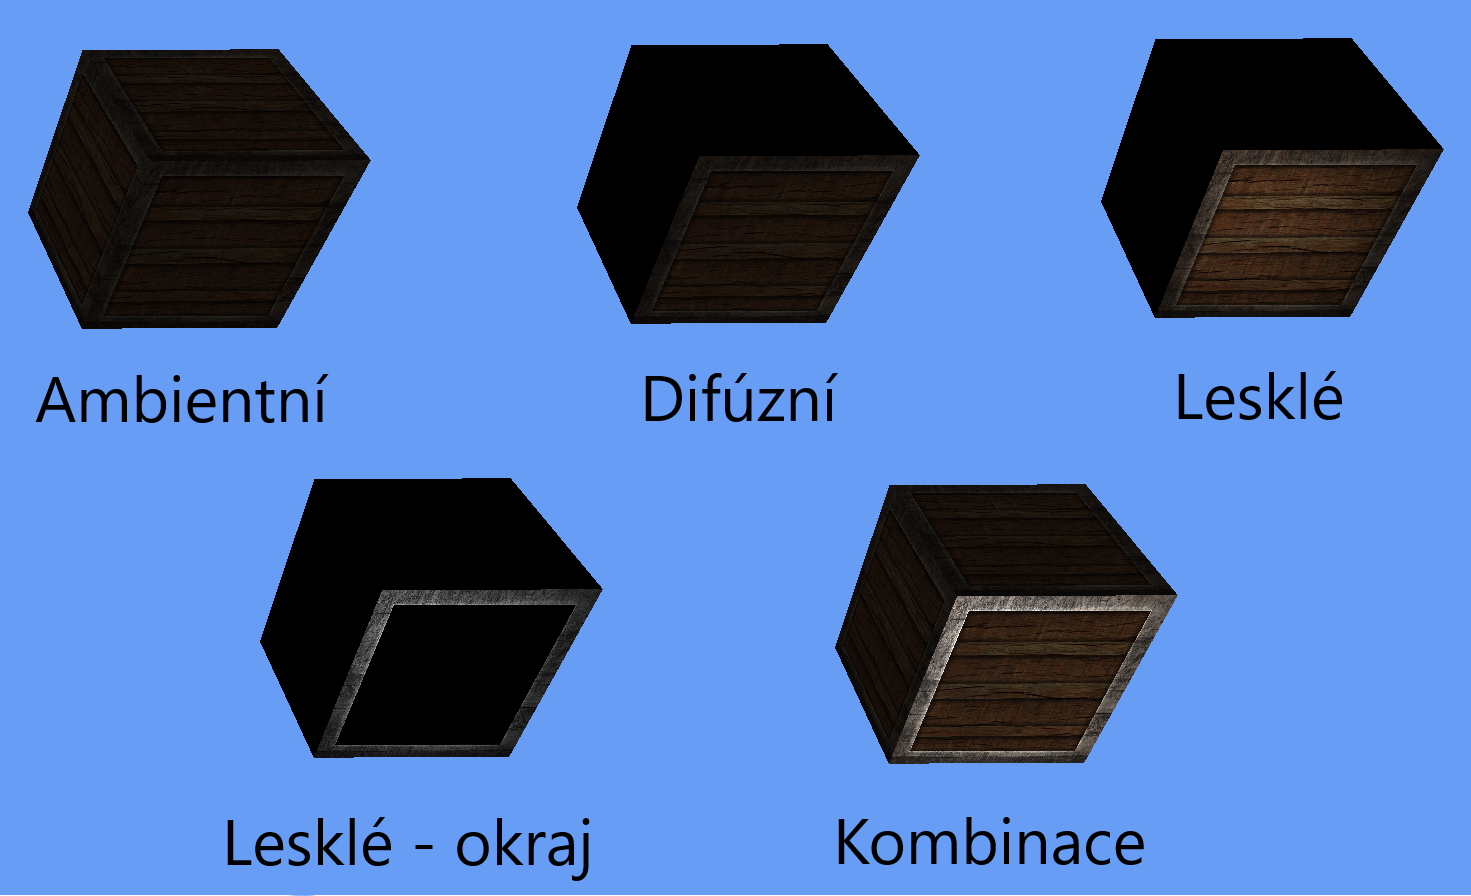
\includegraphics[width=\textwidth]{images/phong}
	\caption[Phongův osvětlovací model]{Phongův osvětlovací model}\label{fig:phong}
\end{figure}

\subsection{Materiál objektu}

Obrázek~\ref{fig:phong} zobrazuje dvě možnosti použití lesklého světla. Bedna jejíž celý povrch odráží světlo působí nepřirozeným dojmem. V reálném světě dřevo světlo neodráží\footnote{Dřevo s naleštěným povrchem světlo odrážet může, tato povrchová úprava však pravděpodobně nebude aplikována na přepravní bednu.}. Lesknout by se měl pouze její kovový okraj, a to jen v místech kde není poškozen.

Tento problém je vyřešen předáním nové textury pro lesklé světlo. Řádek vyhodnocující barvu lesklého světla nebude používat texturu \texttt{texture\_diffuse1}, na místo ní využije \texttt{texture\_specular1}.

\begin{verbatim}
vec3 specular = spec * light.specular * 
    vec3(texture(texture_specular1, TexCoord));
\end{verbatim}

Lesklá textura nemusí definovat barvu odrazu -- odražené světlo má barvu zdroje světla, ale pouze její intenzitu. Dřevěná část textury má černou barvu (žádný odraz), kovová část je převedena do černo-bílého spektra~\cite{lopgl_light_maps}.

Pokud objekt nemá používat lesklé odrazy, nemusí být textura definována. Při změně nastavení textur, jsou všechny navázané textury odpojeny (unbound from texture samplers). Následně jsou navázané všechny definované textury.

\begin{verbatim}
unsigned int diffuseNr = 1;
unsigned int specularNr = 1;
for (unsigned int i = 0; i < Textures.size(); i++) {
    // retrieve texture number (the N in diffuse_textureN)
    std::string number;
    std::string name = Textures[i].Type_;
    if (name == "texture_diffuse")
        number = std::to_string(diffuseNr++);
    else if (name == "texture_specular")
        number = std::to_string(specularNr++);

    // now set the sampler to the correct texture unit
    shader.SetInteger((name + number).c_str(), i);
    Textures[i].Bind(i);
}
\end{verbatim}

Pokud dojde ke čtení z textury, která není navázána, bude vrácena černá barva, představující nulový lesk~\cite{unbound_texture}.

\subsection{Zdroje světla}

Aktuální implementace představuje bodový zdroj světla, jehož intenzita neklesá s uraženou vzdáleností. Tento model nereprezentuje reálné chování světla. Zavedené jsou dva nové druhy světla:

\begin{itemize}
\item Globální osvětlení --- Představuje zdroj světla nekonečně vzdálený od scény, jehož paprsky jsou rovnoběžné a jeho intenzita se nemění. Jeho pomocí lze modelovat objekty jako je Slunce. 

\item Bodové osvětlení --- Paprsky se šíří všemi směry. Intenzita klesá s uraženou vzdáleností.
\end{itemize}

\subsubsection{Globální světlo}

Pro výpočet globálního světla není potřeba jeho poloha, pouze směrový vektor jeho paprsků, definovaný směrem od zdroje světla. Při výpočtu intenzity světla byl použit směr od fragmentu ke světlu. Jedinou změnou oproti dosavadnímu výpočtu je převrácení jeho směru.

\begin{verbatim}
float globalInt = 
    max(dot(norm, normalize(-light.globalDir)), 0.0);
vec3 global = globalInt * light.global * 
    vec3(texture(texture_diffuse1, TexCoord));
\end{verbatim}

\subsubsection{Bodové světlo}

Intenzitu světla je možné snižovat lineárně s vzdáleností, kterou urazí. Toto řešení zajistí nižší nasvícení vzdálených objektů, a však vypadá poněkud uměle. Světla v reálném světě jsou z pravidla velmi jasné, pokud se nacházíme v jejich blízkosti. Jejich jas velice rychle klesá s narůstají vzdáleností. V určitém bodě se klesání zpomalí a přibližuje se k nule.

K výpočtu útlumu světla lze použít následující rovnici~\cite{lopgl_light_casters}:

$$ F_{att} = \frac{1.0}{K_c + K_l * d + K_q * d^2} $$

Proměnná \textit{d} reprezentuje vzdálenost fragmentu od zdroje světla. Dále jsou nastaveny tři konstanty:

\begin{itemize}
\item $K_c$ --- Konstantní složka. Obvykle je ponechána na hodnotě 1. Zajišťuje, aby hodnota jmenovatele neklesla pod 1 a nedošlo k navýšení intenzity světla.

\item $K_l$ --- Lineární složka. 

\item $K_q$ --- Kvadratická složka.
\end{itemize}

Graf~\ref{fig:lum} zobrazuje porovnání hodnot intenzity světla danou rovnicí útlumu (oranžová křivka) a lineární závislostí na vzdálenosti (šedá přímka).

\begin{figure}\centering
	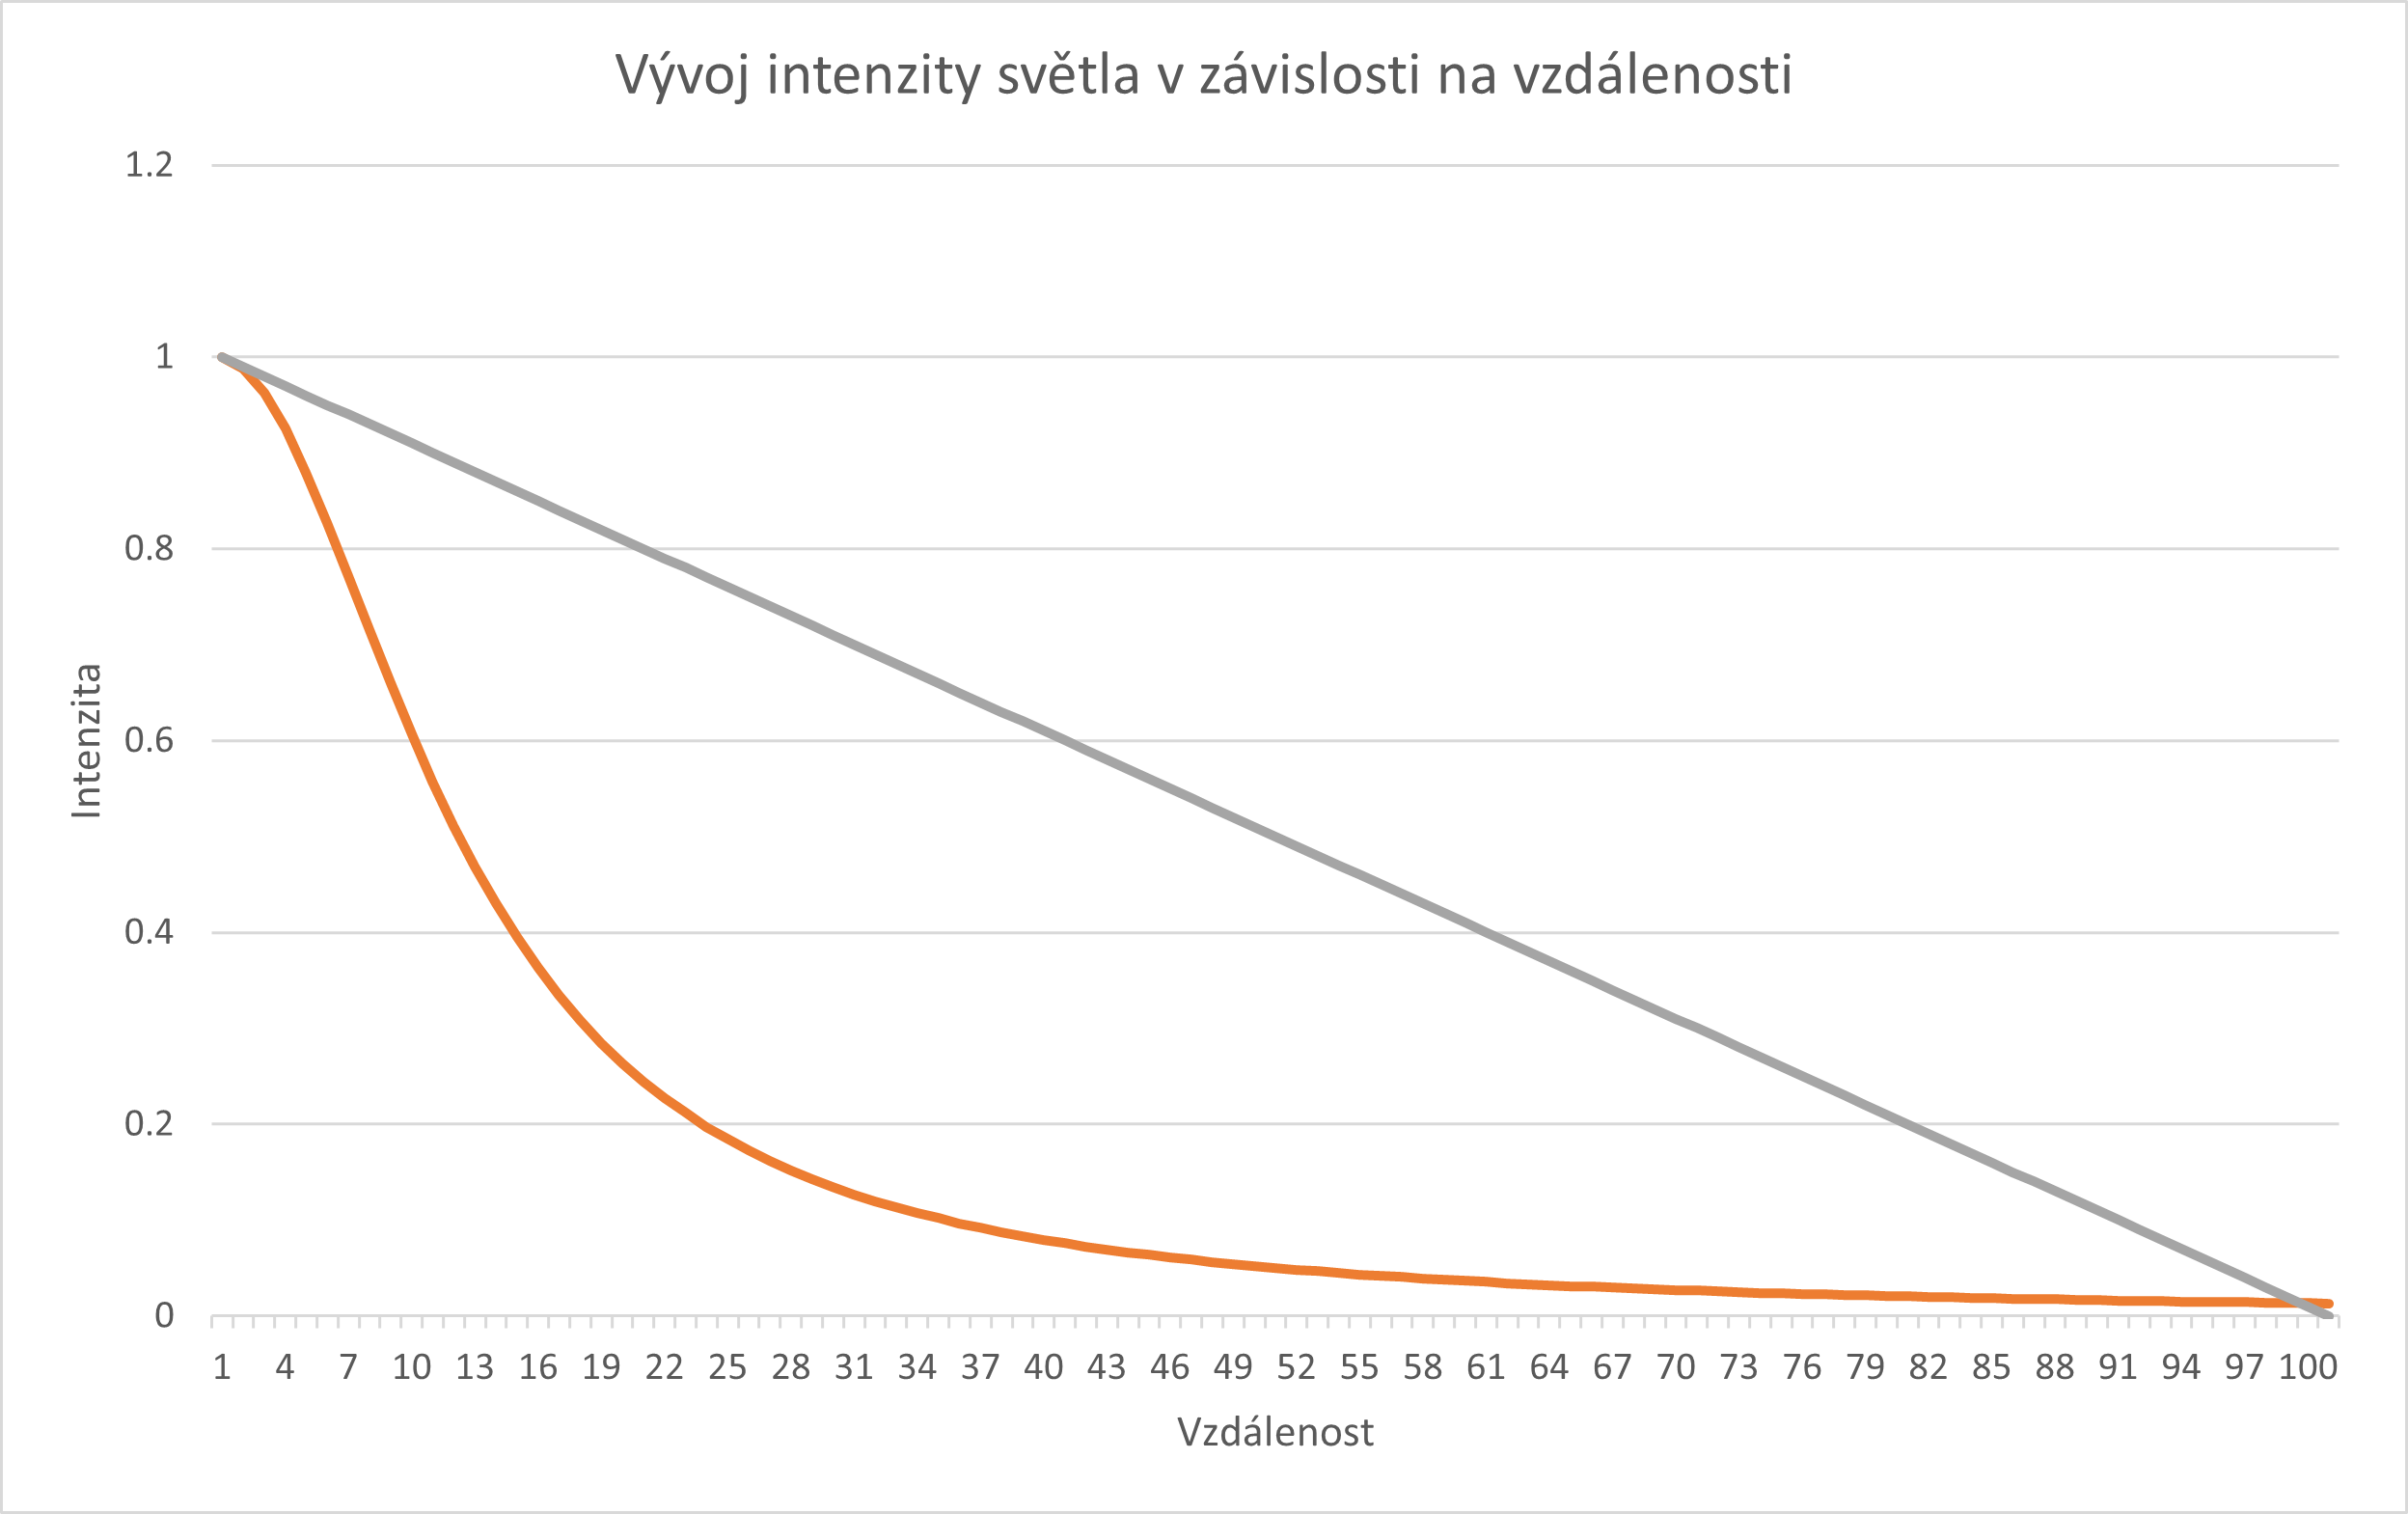
\includegraphics[width=\textwidth]{images/lum}
	\caption[Graf intenzity světla v závisloti na vzdálenosti]{Graf intenzity světla v závisloti na vzdálenosti}\label{fig:lum}
\end{figure}

Hodnoty parametrů jsou určeny požadovaným dosvitem světla. Parametr $K_c = 1$, $K_l = 0,045$ a $K_q = 0,0075$~\cite{ogre_att}. Lineární rovnice má tvar:

$$ F_{att} = \frac{100 - d}{100} $$

Obrázek~\ref{fig:light} ve své levé části zobrazuje scénu vykreslenou pomocí rovnice útlumu. Pravá část snižuje intenzitu světla lineárně.

\todo{Je tento obrázek potřeba?}

\begin{figure}\centering
	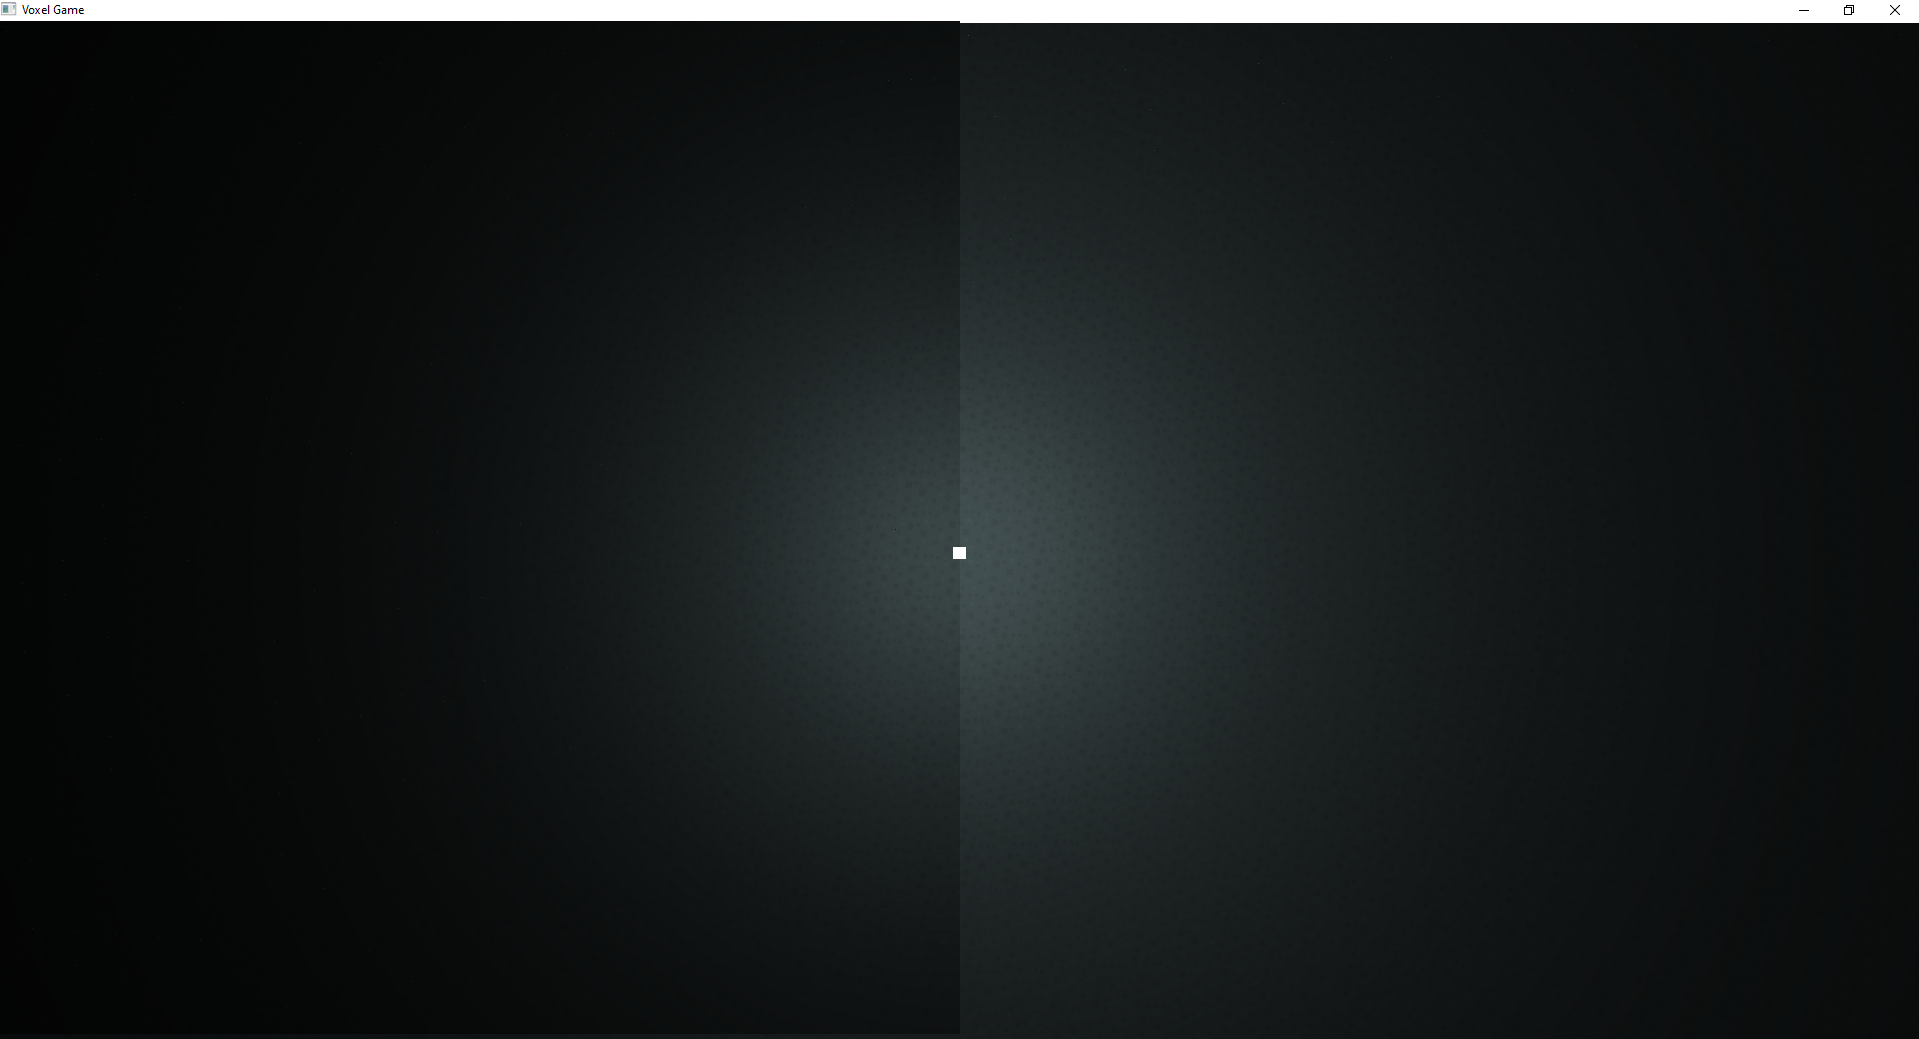
\includegraphics[width=\textwidth]{images/light}
	\caption[Intenzita světla v závisloti na vzdálenosti]{Intenzita světla v závisloti na vzdálenosti}\label{fig:light}
\end{figure}

% % % % % % % % % % % % % % % % % % % % % % % % % % % % 
% % Stíny
% % % % % % % % % % % % % % % % % % % % % % % % % % % % 

\chapter{Mapování stínů}

V levé části obrázku~\ref{fig:shadows_intro} lze vidět scénu nasvícenou globálním světlem. Každý blok scény je nasvícen individuálně a ignoruje ostatní bloky, které by ho mohli zastiňovat. Tento efekt působí velice nereálně zvláště v podrostu džungle a~pod širokými korunami akácií, které jsou nasvíceny plným světlem. Přidáním stínů lze docílit věrohodnější reprezentace reálného světa a~hráč získá lepší představu o pozici bloků vůči sobě.

\begin{figure}\centering
	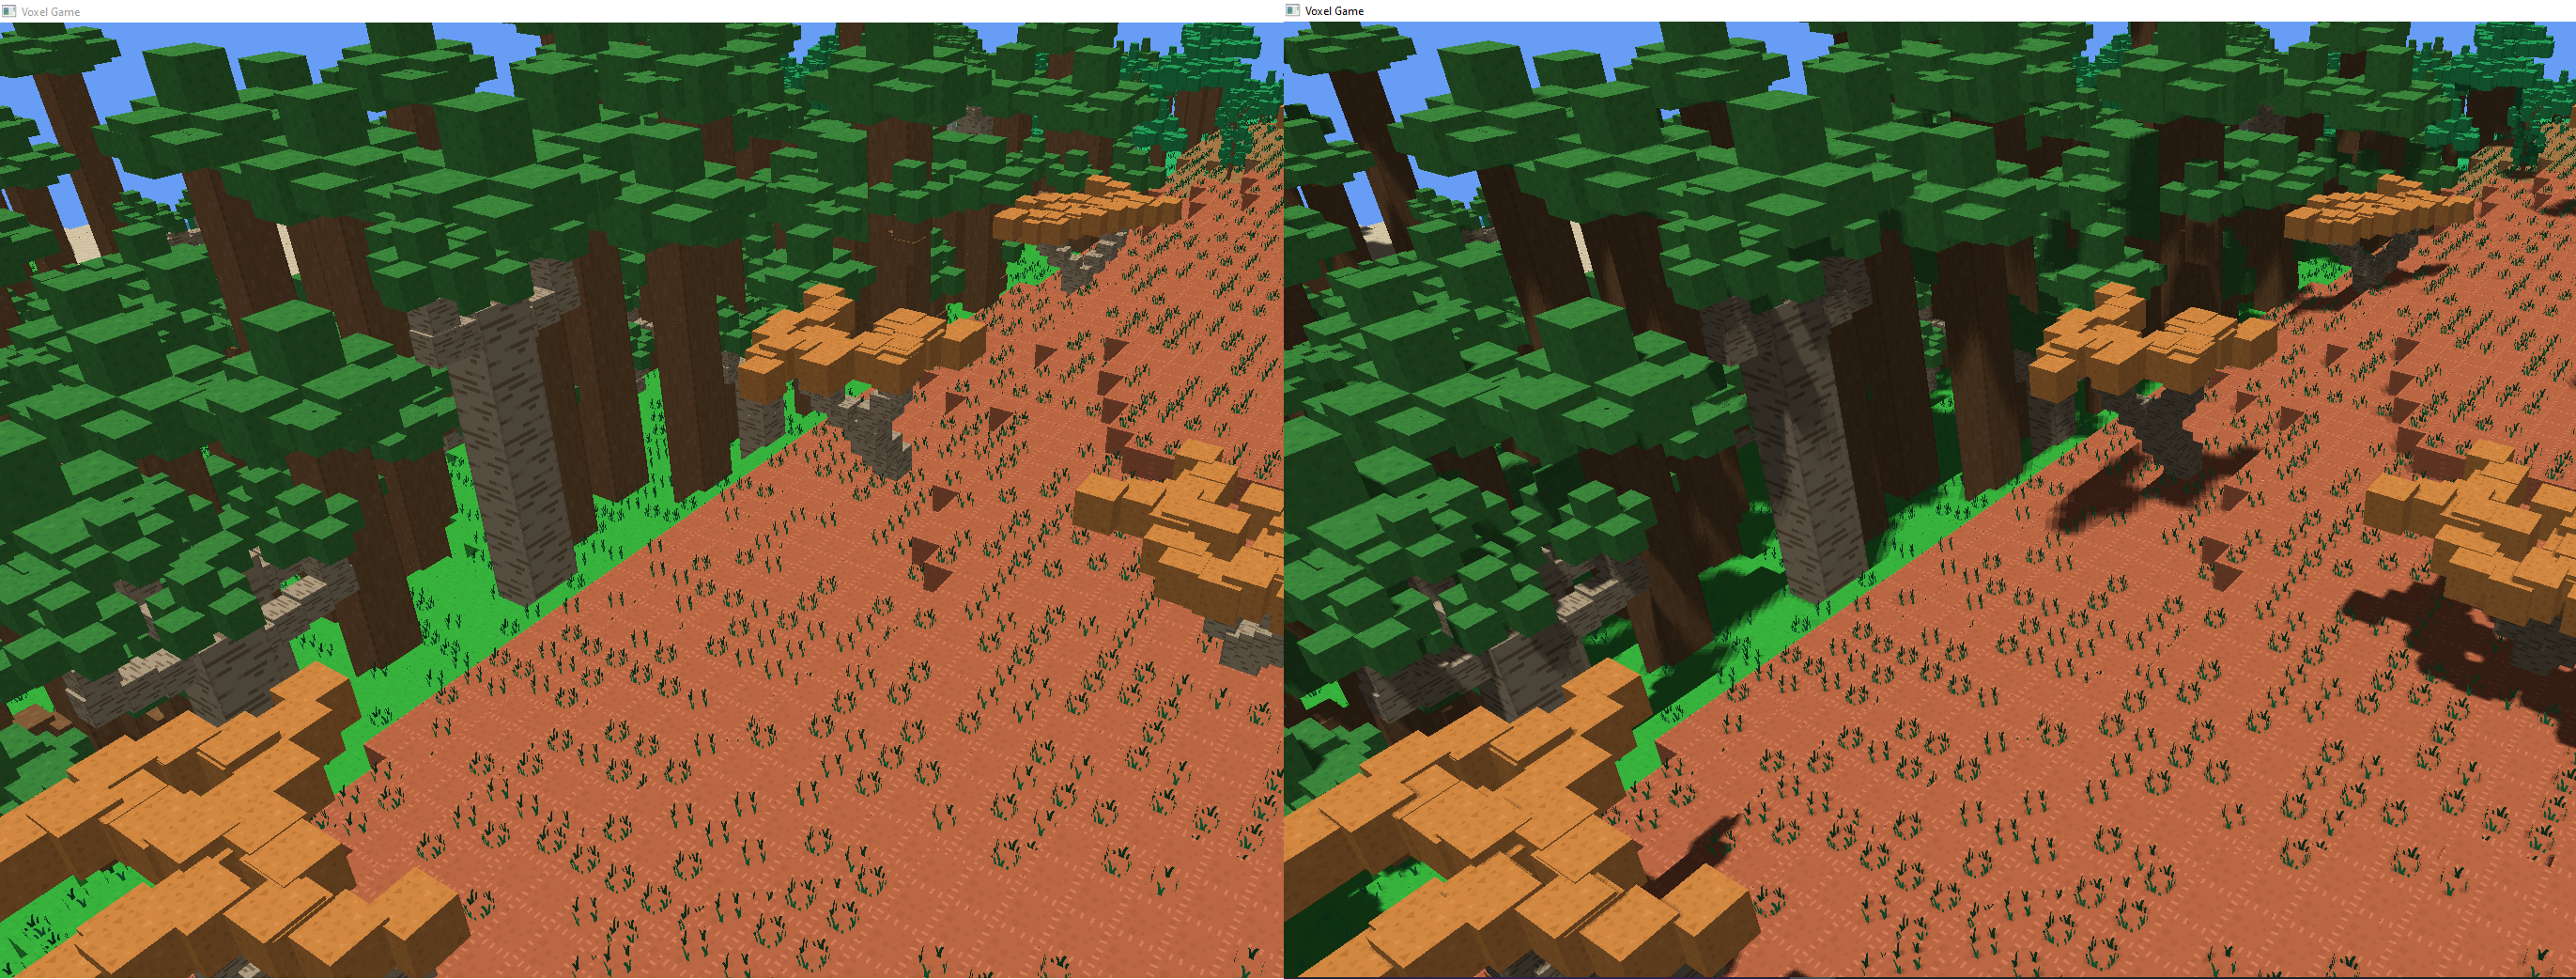
\includegraphics[width=\textwidth]{images/shadows/intro}
	\caption[Porovnání scnény bez stínu a se stíny]{Porovnání scnény bez stínu a se stíny}\label{fig:shadows_intro}
\end{figure}
\todo{Moc siroky obrazek}

Trasování tisíců paprsků světla v reálném čase je výpočetně neúnosné. Proto je použita technika mapování stínů, využívající hloubkového bufferu grafické karty. Scéna je nejprve vykreslena z pohledu světla a hodnoty hloubky fragmentů uloženy do textury nazývané mapa stínů.

Pro druhé vykreslovací kolo, je mapa stínů předána fragment shaderu. Ten provede transformaci pozice fragmentu z prostoru světa (world space) na pozici v prostoru světla a~porovná jeho hloubku s hloubkou uloženou v mapě stínů~\cite{lopgl_shadows}.

\section{Vykreslení mimo obrazovku}

OpenGL umožňuje změnit objekt, do kterého se uloží výsledek vykreslovacího řetězce. V~základním nastavení to je obrazovka hráče. Toto nastavení lze změnit vytvořením nového framebufferu a textury, do které se bude vykreslovat.

Textura může mít jiné rozlišení, než má okno, na které je vykreslována scéna. Zvětšením rozlišení se zlepší kvalita stínů, na úkor rychlosti vykreslování. Mapa stínů nemusí pokrývat veškeré objekty, které hráč vidí. Proto je textuře nastaven okraj, s maximální hloubkou. Při čtení pixelů mimo texturu se díky parametru \texttt{GL\_CLAMP\_TO\_BORDER} vrátí maximální hloubka a vykreslovaný objekt nebude mít stín.

\begin{verbatim}
Texture_.Generate(Width, Height, nullptr);
glBindTexture(GL_TEXTURE_2D, Texture_.Id);
// set no shadow outside of the shadow map
constexpr float borderColor[] = { 1.0f, 1.0f, 1.0f, 1.0f };
glTexParameterfv(
    GL_TEXTURE_2D, GL_TEXTURE_BORDER_COLOR, borderColor);
glBindTexture(GL_TEXTURE_2D, 0);
\end{verbatim}

Pro vykreslení je vygenerován nový framebuffer, jemuž je textura předána jako hloubková složka. Při výpočtu stínu není potřeba buffer pro barvu. Framebuffer objekt by bez něj nebyl kompletní, a proto se musí explicitně nastavit \texttt{glDrawBuffer} a~\texttt{glReadBuffer} na \texttt{GL\_NONE}. 

\begin{verbatim}
// attach to framebuffer
glGenFramebuffers(1, &FBO_);
glBindFramebuffer(GL_FRAMEBUFFER, FBO_);
glFramebufferTexture2D(
    GL_FRAMEBUFFER, GL_DEPTH_ATTACHMENT,
    GL_TEXTURE_2D, Texture_.Id, 0);
glDrawBuffer(GL_NONE);
glReadBuffer(GL_NONE);
\end{verbatim}

Před vykreslením se musí nastavit velikost zobrazovacího zařízení, na které se má scéna vykreslit. V tomto případě velikost textury mapy stínů.

\begin{verbatim}
glViewport(0, 0, Width, Height);
\end{verbatim}

Pro vykreslení do mapy stínů je použit shader, který transformuje vertex do souřadnic světla. A předá pozici textury k dalšímu zpracování.

\begin{verbatim}
TexCoord = vec2(aTexCoord.x + shift.x, aTexCoord.y + shift.y);
gl_Position = lightSpaceMatrix * model * vec4(aPos, 1.0);
\end{verbatim}

Fragment shader vyřadí všechny průhledné fragmenty a zapíše jejich hloubku.

\begin{verbatim}
float alpha = vec4(texture(texture_diffuse1, TexCoord)).a;
if (alpha < 0.05)
    discard;

gl_FragDepth = gl_FragCoord.z;
\end{verbatim}

\section{Vykreslení stínu}

K vykreslení stínu je použit shader z kapitoly o světle. Globální složka světla je vynásobena hodnotou \textit{(1 -- shadow)}, kde \textit{shadow = 1} znamená maximální stín a~\textit{shadow = 0} žádný stín.

\begin{verbatim}
float shadow = ShadowCalculation(fs_in.FragPos, dotLightNormal);
vec3 global = 
    (1 - shadow) * globalInt * light.global * 
    vec3(texture(texture_diffuse1, TexCoord));
\end{verbatim}

Funkce \texttt{ShadowCalculation} vrátí hodnotu 1, pokud je hloubka fragmentu větší než hodnota v mapě stínů, jinak vrátí 0.

\begin{verbatim}
// perform perspective divide
vec3 projCoords = fragPosLightSpace.xyz / fragPosLightSpace.w;
// transform to [0,1] range
projCoords = projCoords * 0.5 + 0.5;
float closestDepth = texture(shadowMap, projCoords.xy).r; 
float currentDepth = projCoords.z;
return currentDepth > closestDepth  ? 1.0 : 0.0;
\end{verbatim}

Scéna~\ref{fig:shadows_acne} je vykreslena s použitím toho shaderu. Stíny stromů jsou správně vykresleny, oko diváka však přitáhnou artefakty vzniklé při výpočtu stínu, nazývající se stínové akné.

\begin{figure}\centering
	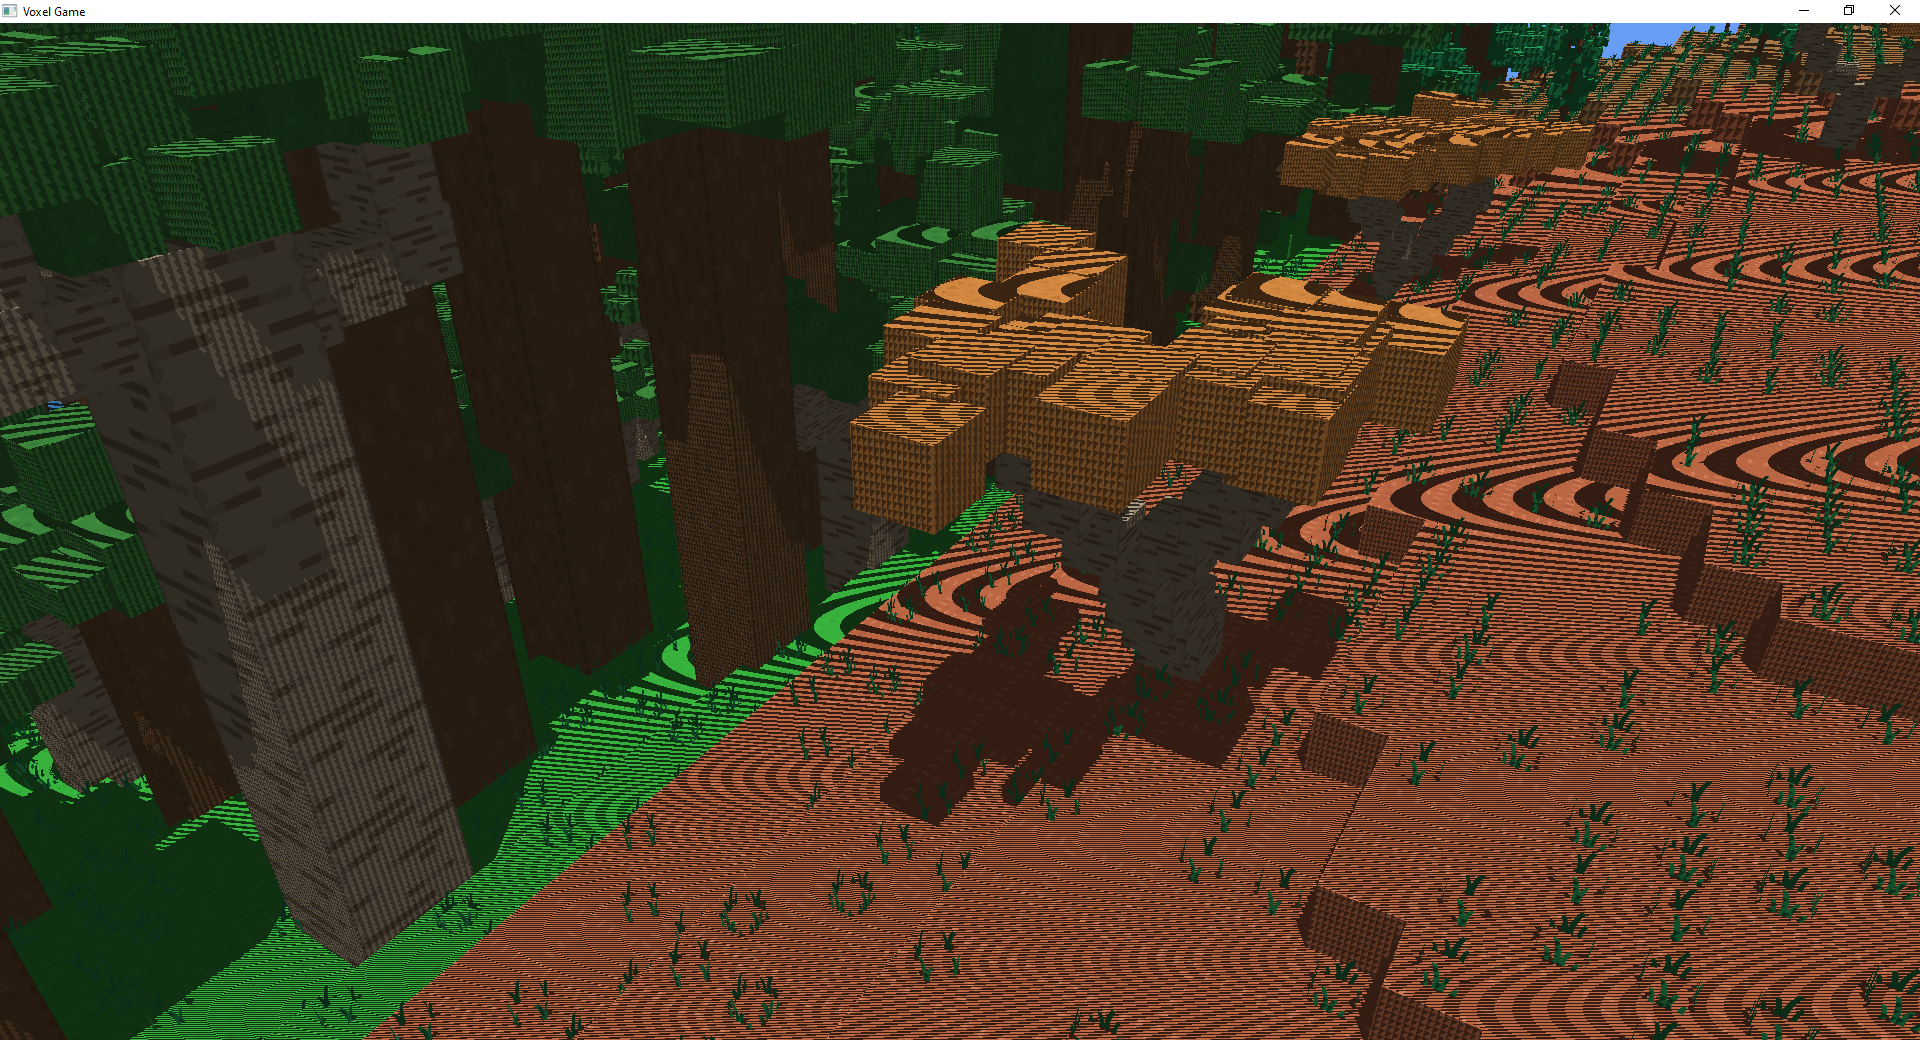
\includegraphics[width=\textwidth]{images/shadows/acne}
	\caption[Stínové akné]{Stínové akné}\label{fig:shadows_acne}
\end{figure}

\section{Stínové akné}

Viditelné artefakty vznikají na površích, které by neměly mít stín. Problém ilustruje diagram~\ref{fig:shadows_diag_acne}, kde je mapa stínů promítnuta na vodorovný povrch. Každá šipka představuje jeden paprsek světla -- texel mapy stínů -- dopadající na povrch. Omezené rozlišení mapy stínů má za důsledek, že několik fragmentů může číst hodnotu hloubky ze stejného texelu. Fragmenty nacházející se nad žlutou křivkou nemají stín, fragmenty nacházející se pod ní stín mají. 

\begin{figure}\centering
	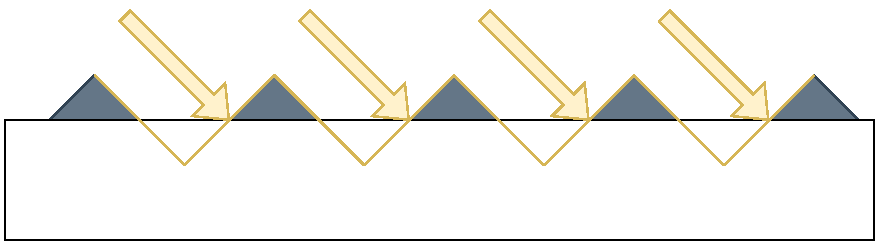
\includegraphics[width=\textwidth]{images/shadows/diag_acne}
	\caption[Důvod vzniku stínového akné]{Důvod vzniku stínového akné}\label{fig:shadows_diag_acne}
\end{figure}

K tomuto problému dochází v přídě, kdy světlo dopadá na povrch pod úhlem. V jednoduché scéně, kdy je slunce nad hlavou hráče, by k tomuto problému nedocházelo. Takové scény nejsou vizuálně zajímavé a značně by omezovali možnosti enginu.

Problém lze vyřešit posunutím mapy stínů (nebo povrchu objektu) tak, aby se texely mapy stínů nenacházely na povrchem objektu, viz diagram~\ref{fig:shadows_diag_acne_fix}.

\begin{figure}\centering
	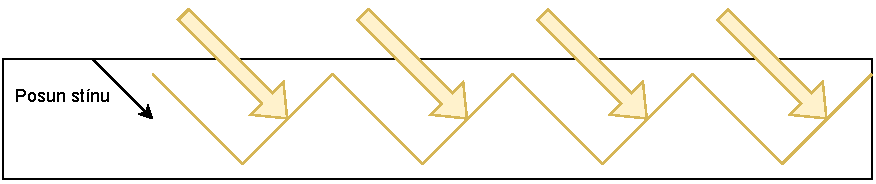
\includegraphics[width=\textwidth]{images/shadows/diag_acne_fix}
	\caption[Zamezení vzniku stínového akné]{Zamezení vzniku stínového akné}\label{fig:shadows_diag_acne_fix}
\end{figure}

Pro posun mapy lze zvolit konstantu.

\begin{verbatim}
float bias = 0.0085;
float shadow = currentDepth - bias > closestDepth ? 1.0 : 0.0;
\end{verbatim}

Toto řešení funguje pro světlo dopadající na povrch pod stejným úhlem. Pokud se změní zdroj světla nebo orientace objektu, nemusí být konstanta dostatečně velká a problém se bude opakovat. Robustnějším řešením je vypočítat odchylku -- \texttt{bias} -- podle úhlu dopadu světla, který bude největší pro světlo dopadající na povrch pod ostrým úhlem a nejmenší pro světlo dopadající kolmo.

\begin{verbatim}
float bias = max(0.0085 * (1.0 - dotLightNormal), 0.00085);
\end{verbatim}

\section{Ostré stíny}

Při pohledu na scénu~\ref{fig:shadows_pcf_hard} lze odhalit nedostatečné rozlišení mapy stínů. Několik vykreslovaných fragmentů se namapuje na jeden texel z mapy stínů. Výsledkem jsou zubaté hrany stínu s velmi ostrým přechodem. Řešení, které nevyžaduje zvětšení rozlišení je procentuálně bližší filtrování (percentage--closer filtering -- PCF).

\begin{figure}\centering
	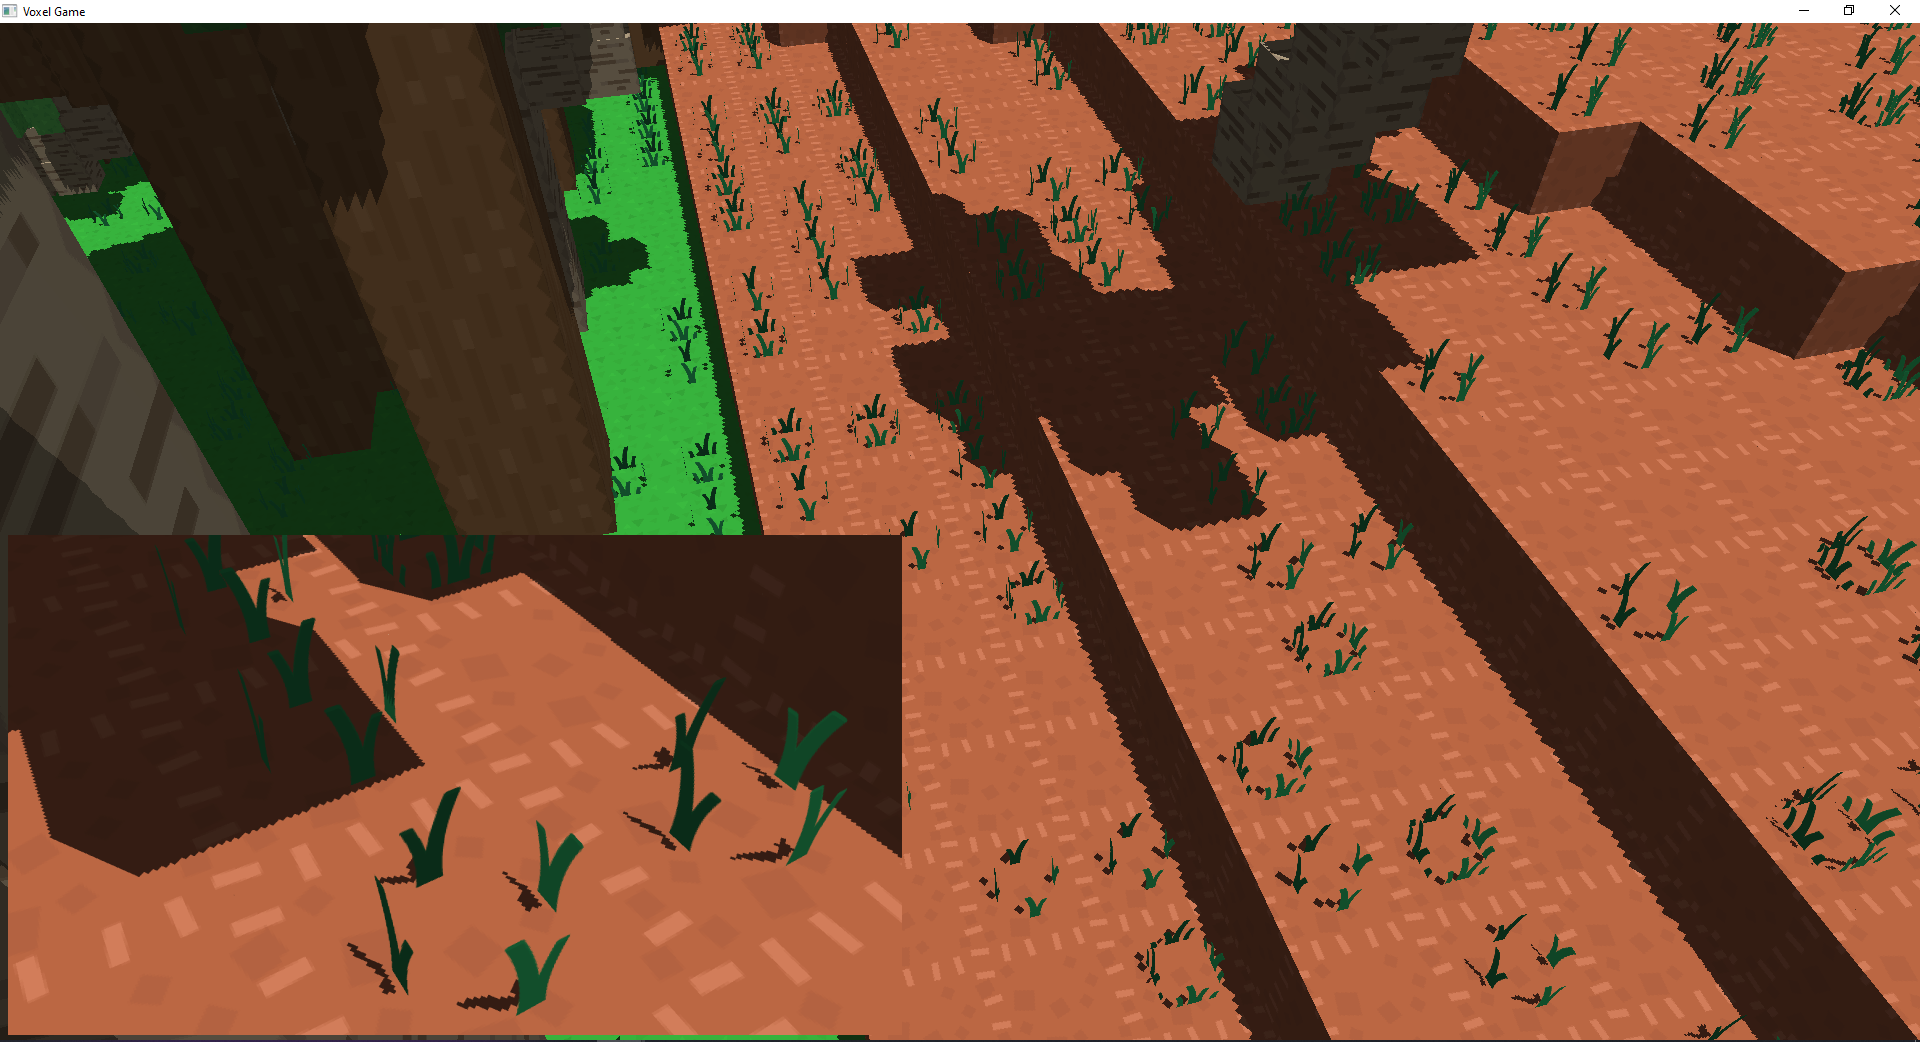
\includegraphics[width=\textwidth]{images/shadows/pcf_hard}
	\caption[Ostrá hrana stínu]{Ostrá hrana stínu}\label{fig:shadows_pcf_hard}
\end{figure}

Technika PCF produkuje jemnější stíny. Ty se jeví méně hranaté a zubatý efekt není tak výrazný. PCF zahrnuje více způsobu filtrování, jehož základem je vícenásobné čtení vzorků z textury stínu a jejich zprůměrování. Jednoduchá technika je čtení hodnot ve čtverci kolem zpracovávaného texelu.

\begin{verbatim}
float shadow = 0.0;
vec2 texelSize = 1.0 / textureSize(texture_shadow, 0);
for(int x = -1; x <= 1; ++x) {
    for(int y = -1; y <= 1; ++y)  {
        float pcfDepth = texture(
            texture_shadow,
            projCoords.xy + vec2(x, y) * texelSize).r;
        shadow += currentDepth - bias > pcfDepth ? 1.0 : 0.0;        
    }    
}
shadow /= 9.0;
\end{verbatim}

Scéna~\ref{fig:shadows_pcf_soft} je vykreslena při použití 9~vzorků. Při pohledu z~dálky lze pozorovat lepší výsledky, zuby stínů nejsou tolik patrné, jako při použití jednoho vzorku. Při bližším pohledu na stébla trávy, lze pozorovat rozšíření stínu o~jeden texel. Štíhlé textury již nevrhají přesné stíny, výměnou za zlepšení pohledu z~dálky, kdy byl vrhaný stín nepřesný (velikost texelu neodpovídala velikosti textury) a~byla vykreslena pouze jeho část s~velice ostrým přechodem.

\begin{figure}\centering
	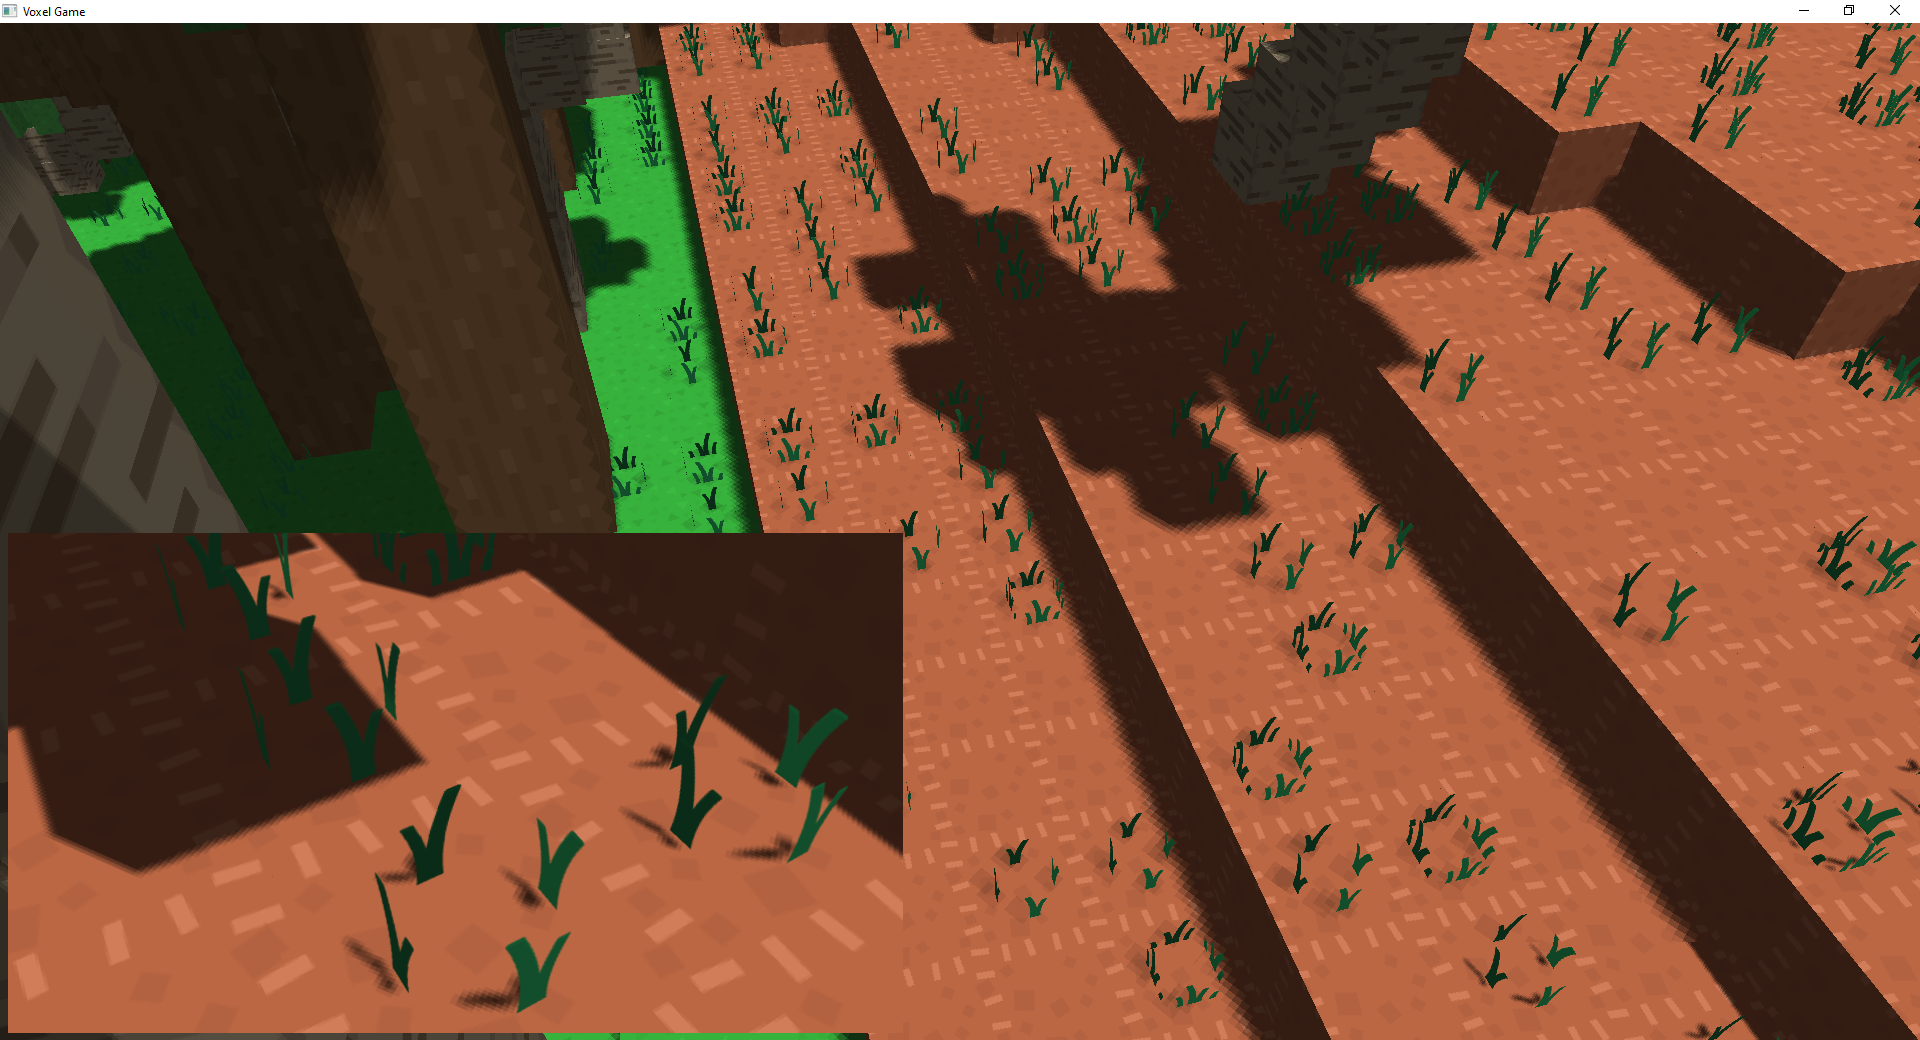
\includegraphics[width=\textwidth]{images/shadows/pcf_soft}
	\caption[Měkká hrana stínu]{Měkká hrana stínu}\label{fig:shadows_pcf_soft}
\end{figure}

\section{Pozice mapy stínů na scéně}

Mapa stínů musí být posouvána podle pozice kamery v herním světě. Objekty jsou generovány kolem postavy hráče a pokud se hráč posune od počátku světa, objekty budou smazány a nemohou vrhat stíny. Mapa stínů má však omezené rozlišení a stínováním objektů, které jsou vygenerované, ale hráč je nemá šanci vidět (jsou například za ním), se snižuje kvalita stínů. Pro maximální využití dostupného rozlišení stačí pokrýt pouze objekty, které může hráč v daném snímku vidět. Viditelná část světa je určena maticí pohledu (view) a maticí projekce (projection). Tyto matice tvoří frustum, ve kterém budou objekty viditelné. Toto frustum je potřeba obsáhnout frustem světla s co nejmenšími přesahy. Tato skutečnost ve 2D světě, je ilustrována na obrázku~\ref{fig:shadows_frustum_fit}.

\begin{figure}\centering
	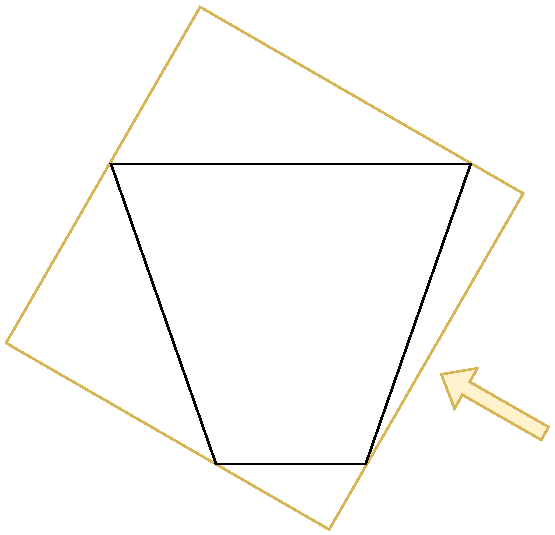
\includegraphics[width=0.7\textwidth]{images/shadows/frustum_fit}
	\caption[Frustum světla okolo frusta kamery]{Frustum světla okolo frusta kamery}\label{fig:shadows_frustum_fit}
\end{figure}

\subsection{Souřadnice frusta kamery}

Matice pohledu a projekce transformují souřadnice světa na normalizované souřadnice zařízení (NDC – normalized device coordinates). Každá souřadnice na jedné ze tří os NDC nabývá hodnot $[-1, 1]$. Do souřadnic světa je lze převést vynásobením inverzí matic pohledu a projekce~\cite{lopgl_csm}.

$$
v_{NDC} = M_{proj} * M_{view} * v_{world}
$$
$$
v_{world} = (M_{proj} * M_{view})^{-1} * v_{NDC}
$$

Pro vytvoření frusta světla, je nutné zjistit souřadnice rohů frusta kamery. Díky nim je možné přesně zjistit jakou část světa má frustum světla pokrývat. Souřadnice jsou vypočítané následujícím způsobem:

\begin{verbatim}
std::vector<glm::vec4> Helpers::Math::FrustumCornersWordSpace(
  const glm::mat4& proj, const glm::mat4& view) {
    const auto inv = glm::inverse(proj * view);

    std::vector<glm::vec4> frustumCorners;
    for (unsigned int x = 0; x < 2; ++x) {
        for (unsigned int y = 0; y < 2; ++y) {
            for (unsigned int z = 0; z < 2; ++z) {
                const glm::vec4 pt =
                    inv * glm::vec4(
                        2.0f * x - 1.0f, 2.0f * y - 1.0f,
                        2.0f * z - 1.0f, 1.0f);
                frustumCorners.emplace_back(pt / pt.w);
    }}}

    return frustumCorners;
}
\end{verbatim}

\subsection{Matice pohledu a projekce světla}

Pro výpočet matice pohledu světla je potřeba zjistit bod, který je ve středu stínované oblasti. Tento bod se nachází ve středu frusta kamery. A je ho možné získat zprůměrováním pozic rohů frusta.

\begin{verbatim}
glm::vec3 Helpers::Math::FrustumCenter(
  const std::vector<glm::vec4>& corners) {
    auto center = glm::vec3(0.0f);
    for (const auto& v : corners) {
        center += glm::vec3(v);
    }
    center /= corners.size();

    return center;
}
\end{verbatim}

Matice pohledu je získána pomocí funkce \texttt{glm::lookAt} a směru světla.

\begin{verbatim}
const auto lightView = glm::lookAt(
    center,
    center + lightDir,
    glm::vec3(0.0f, 1.0f, 0.0f));
\end{verbatim}

Pro stínování scény je použito globální světlo. K výpočtu matice projekce bude tedy použita funkce glm::ortho zaručující ortografickou projekci. Pro výpočet je nutné zjistit parametry \texttt{left, right, bottom, top, zNear} a~\texttt{zFar}.

Při pohledu od zdroje světla bude jeho frustum osově zarovnaný kvádr, těsně objímající frustum kamery. Rohy kamery lze pomocí matice pohledu světla transformovat do souřadnicového systému pohledu světla. Z~těchto transformovaných rohů je vybráno maximum a~minimum v~každé ose, definující frustum světla.

\begin{verbatim}
for (const auto& v : corners) {
    const auto trf = lightView * v;
    minX = std::min(minX, trf.x);
    maxX = std::max(maxX, trf.x);
    minY = std::min(minY, trf.y);
    maxY = std::max(maxY, trf.y);
    minZ = std::min(minZ, trf.z);
    maxZ = std::max(maxZ, trf.z);
}
\end{verbatim}

Před vytvořením matice projekce je potřeba upravit proměnnou \texttt{minZ} a~\texttt{maxZ}, představující blízkou a vzdálenou plochu frusta. S aktuální hodnotou by stíny vrhaly pouze objekty viditelné hráčem. Například stín koruny stromu by se objevil pouze, pokud by ji hráč viděl.

Posunuté hranice frustra by měly pokrývat všechny objekty na scéně. Příliš velkorysým posunutím však dojde ke ztrátě přesnosti mapy stínů. Hranice by tedy měly být posunuté podle aktuální scény, například aby byl vykreslen stín pod nejvyšším stromem, u jehož paty hráč stojí.

\todo{mozna zahodit}

\begin{verbatim}
if (minZ < 0) 
    minZ *= zMult;
else 
    minZ /= zMult;
if (maxZ < 0) 
    maxZ /= zMult;
else 
    maxZ *= zMult;

const glm::mat4 lightProjection = 
    glm::ortho(minX, maxX, minY, maxY, minZ, maxZ);

return lightProjection * lightView;
\end{verbatim}

\section{Kaskádové mapování stínů}

Jednoduché mapování stínů má podstatnou nevýhodu. Pokud chceme rozšířit oblast pokrytou stíny, musíme zvýšit rozlišení mapy stínů. V opačném případě by stíny blízko hráče byly rozkostičkované. Tímto zvyšováním kvality stínů je masivně zatěžováno GPU. Stíny, které jsou vzdálenější od hráče budou mít stejnou kvalitu, jako ty mu blízké. Toto je zbytečné, vzdálenější stíny mohou mít horší kvalitu – hráč bude rozlišovat pouze jejich tvar a existenci, drobné detaily jsou zbytečné. Tento problém řeší kaskádové mapování stínů, skládající se z následujících kroků~\cite{lopgl_csm}.

\begin{enumerate}
\item Rozděl frustum kamery na $n$ subfrust, kde vzdálená plocha frusta $i$ je blízká plocha frusta $i + 1$.

\item Pro každé frustum spočítej matici prostoru světla.
\item Vykresli mapu stínů pro každé frustum.
\item Předej všechny mapy stínu fragment shaderu.
\item Vykresli scénu, kde podle vzdálenosti fragmentu vybereš patřičnou mapu stínů.
\end{enumerate}

Na obrázku~\ref{fig:shadows_frustum_div} je zobrazeno rozdělení frusta kamery na tři části. Velikost částí se zvětšuje s narůstající vzdáleností od blízké plochy kamery. Rozlišení však zůstává stejné, a proto jeden texel mapy stínů bude pokrývat větší plochu světa. Kvalita stínů se proto bude zhoršovat s rostoucí vzdáleností od hráče. Frustum lze rozdělit na libovolný počet částí. S větším počtem dělení, se snižuje viditelnost změny kaskády.

\begin{figure}\centering
	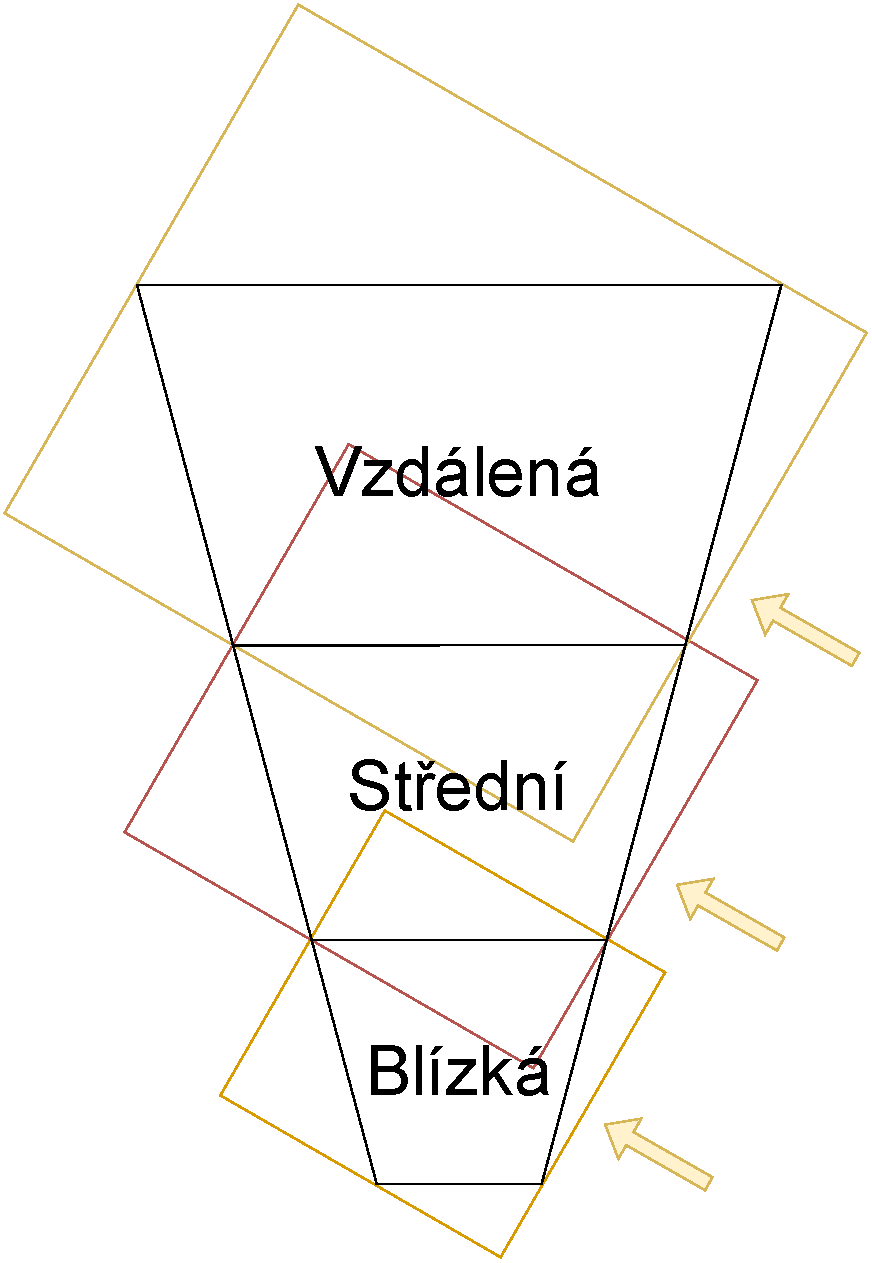
\includegraphics[width=0.7\textwidth]{images/shadows/frustum_div}
	\caption[Rozdělení frusta kamery na tři části]{Rozdělení frusta kamery na tři části}\label{fig:shadows_frustum_div}
\end{figure}

\subsection{Mapy stínů}

Pro práci s více texturami, mající stejný rozměr, OpenGL poskytuje pole 2D textur~\cite{kronos_array_texture}. Práce s polem textur usnadní práci (navázání pouze jedné textury) a umožní dynamické měnění počtu textur. Vytvoření 3D textury~\cite{kronos_3d_texture} probíhá obdobně jako vytvoření 2D textury. Jedním z rozdílů je zadání počtu textur, pro alokaci paměti grafické karty.

K vykreslení do pole textur se používá technika vrstveného vykreslování. V ní je za pomoci geometry shaderu vytvořena nová geometrie pro každou vrstvu map stínů. Pro každou matici světla z kaskády je vytvořen nový trojúhelník, který je pomocí ní transformován, a~nastaveno číslo vrstvy.

\begin{verbatim}
void main() {
    for (int i = 0; i < 3; ++i) {
        gl_Position = lightSpaceMatrices[gl_InvocationID] * 
                      gl_in[i].gl_Position;
        gl_Layer = gl_InvocationID;
        TexCoord = gs_in[i].TexCoord;
        EmitVertex();
    }
    EndPrimitive();
}
\end{verbatim}

Pro vykreslení stínů je použit shader vykreslující mapu stínů s úpravami umožňujícími práci s mapami stínů. Pro zvolení správné matice světla je vypočítána hodnota hloubky fragmentu (v prostoru pohledu kamery), která je následně porovnána se vzdáleností nejbližší změny kaskády.

\begin{verbatim}
vec4 fragPosViewSpace = view * vec4(fragPosWorldSpace, 1.0);
float depthValue = abs(fragPosViewSpace.z);

int layer = CASCADE_COUNT - 1;
for (int i = 0; i < CASCADE_COUNT - 1; ++i) {
    if (depthValue < cascadePlaneDistances[i]) {
        layer = i;
        break;
    }
}
vec4 fragPosLightSpace = 
    lightSpaceMatrices[layer] * vec4(fragPosWorldSpace, 1.0);
\end{verbatim}

Na obrázku~\ref{fig:shadows_csm_acne} lze vidět tři kaskády. V první nedochází k stínovému akné, v druhé je již při bližším pozorování patrné a ve třetí je velice výrazné. K tomuto efektu dochází, protože texel v každé vrstvě pokrývá různě velkou plochu vykreslované geometrie. Proto je potřeba volit odchylku na základě vrstvy. Škálování odchylky inverzní hodnoty vzdálené plochy frusta, produkuje výsledky bez stínového akné.

\begin{verbatim}
float bias = max(0.0085 * (1.0 - dotLightNormal), 0.00085);
if (layer == cascadeCount) {
    bias /= farPlane * 0.008;
}
else {
    bias /= cascadePlaneDistances[layer] * 0.02;
}
\end{verbatim}

\begin{figure}\centering
	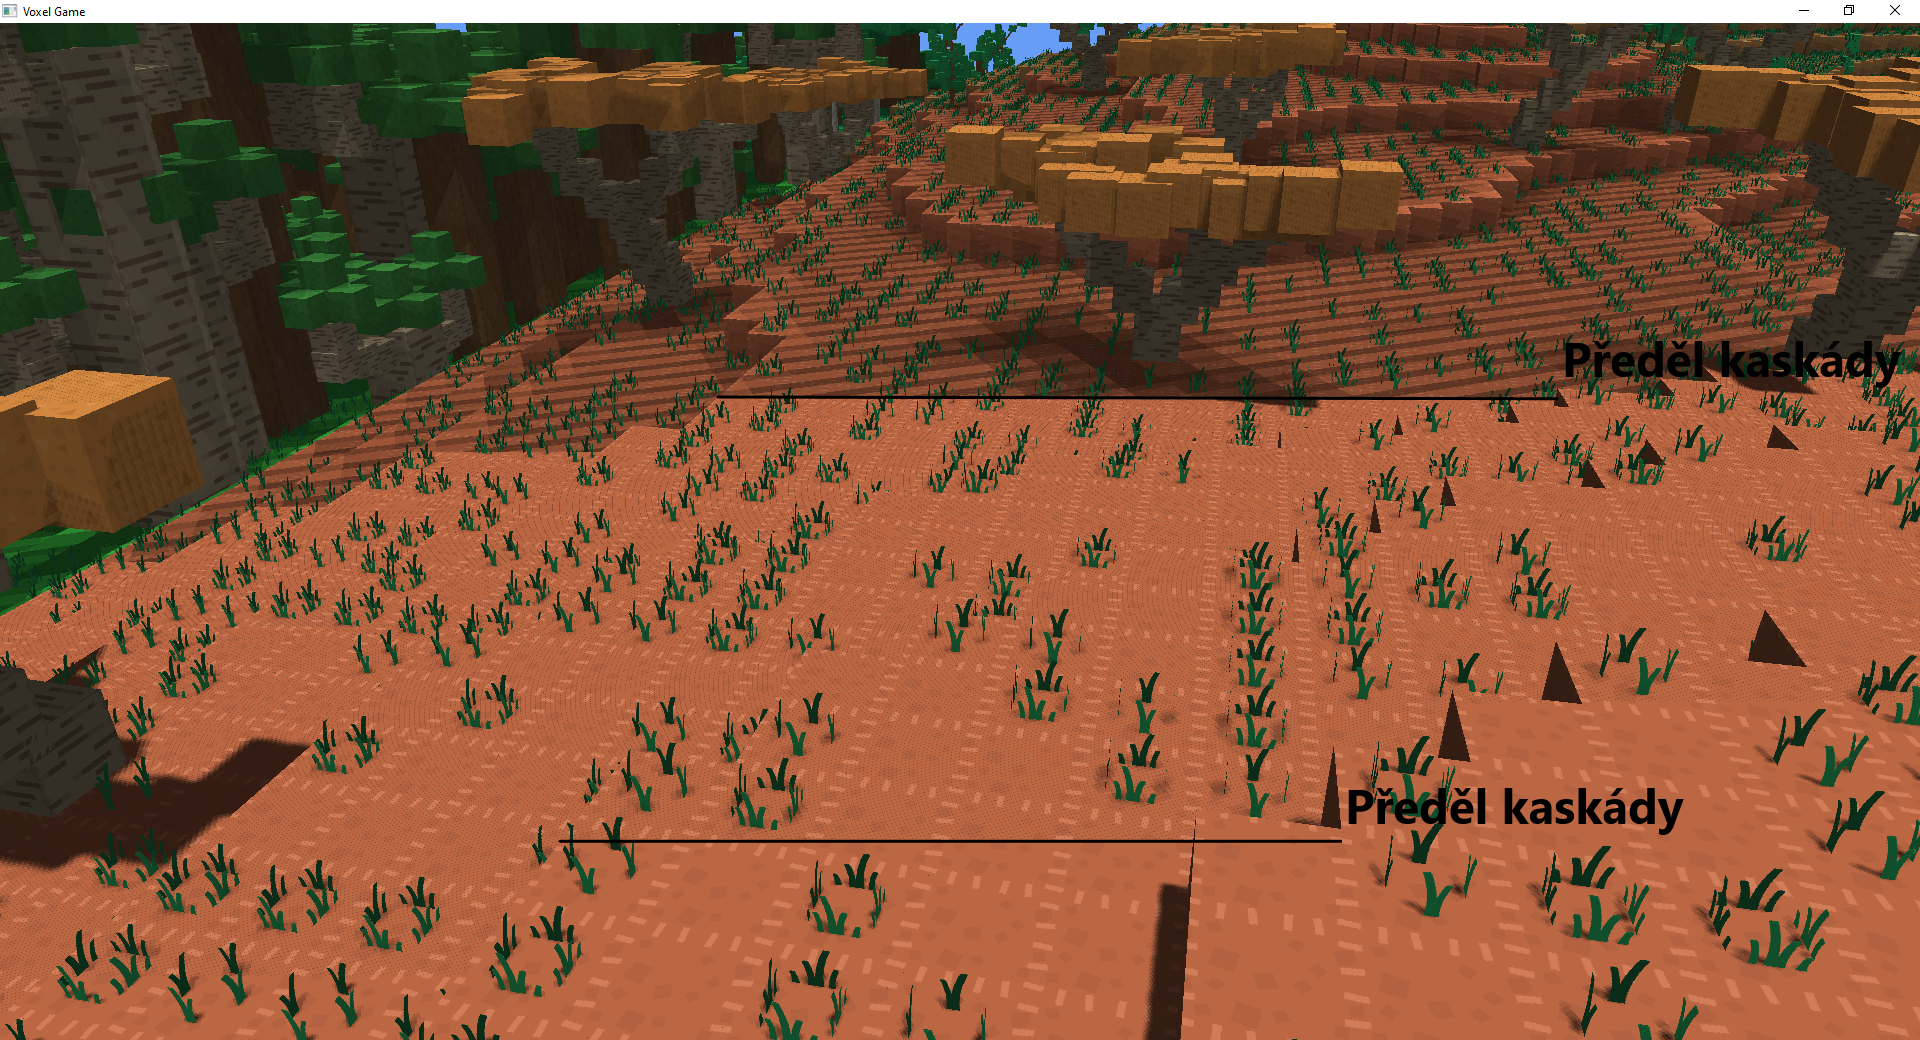
\includegraphics[width=\textwidth]{images/shadows/csm_acne}
	\caption[Velikost stínového akné v závislosti na kaskádě]{Velikost stínového akné v závislosti na kaskádě}\label{fig:shadows_csm_acne}
\end{figure}

Tato technika zavádí větvení, které v shaderech není chtěné. Zároveň neumožnuje dokonalé vylazení odchylky pro jednotlivé kaskády. Odchylka je pevně svázaná s počtem a vzdáleností kaskád. Její výpočet proto může být přesunut na CPU, k definici kaskád. Odchylky jsou předány shaderu pomocí pole a načteny následujícím způsobem.

\begin{verbatim}
float bias = max(0.0085 * (1.0 - dotLightNormal), 0.00085);
bias *= cascadeBiases[layer];
\end{verbatim}

\subsection{Změna počtu kaskád}

Engine umožňuje měnit počet kaskád při běhu programu. Shadery proto musí mít alokované dostatečně velké místo, pro uložení všech matic. Jedinou výjimkou je geometry shader, ve kterém je specifikován počet vyvolání.

\begin{verbatim}
#define CASCADE_COUNT 3
layout(triangles, invocations = CASCADE_COUNT) in;
layout(triangle_strip, max_vertices = 3) out;
\end{verbatim}

Pokud je \texttt{CASCADE\_COUNT} menší, než počet kaskád $n$. $n - 1$ nejvzdálenějších kaskád nebude vykresleno. Pokud je větší, bude plýtván výpočetní čas GPU. Počet kaskád shaderu nemůže být předán parametrem -- vyžaduje běh shaderu. Engine proto umožňuje znovu zkompilovat shadery za běhu a upravit hodnotu maker. Zdrojový kód je po načtení z~disku projit a všechna makra nahrazena specifikovanou hodnotou, kód je následně přeložen. Opakovaný překlad je proveden při změně počtu kaskád.

\begin{verbatim}
ShaderDepth_ = ResourceManager::SetShaderMacros(
  "shadow_csm", {{ "CASCADE_COUNT", std::to_string(levels) }});
\end{verbatim}

Makra jsou použita i ve zbylých shaderech, umožňující alokaci přesného počtu prvků v~poli matic světla, kaskád, atd.

\subsection{Výsledky}

Scéna na obrázku~\ref{fig:shadows_csm} již neobsahuje stínové akné. Lze si všimnout dvou změn kaskád a zhoršení kvality stínů\footnote{Kaskády byly pro viditelnější efekt posunuty k blízké ploše frusta kamery.}. Rozlišení kaskád je nastaveno na 1024~x~1024 pixelů. S~tímto rozlišením je možné pokrýt celou herní scénu v~dostatečné kvalitě. Při použití jednoduché mapy stínů, bylo pokryto pouze malé okolí hráče. Při zvýšení rozlišení na 2048 x 2048 pixelů nebylo možné pokrýt celou scénu s~dostatečným rozlišením, přičemž velikost textury v paměti byla o~třetinu větší než při použití kaskád.

\todo{zmerit vykonost kaskady vs jednoduchy}
% https://stackoverflow.com/questions/28175631/how-to-measure-time-performance-of-a-compute-shader

\begin{figure}\centering
	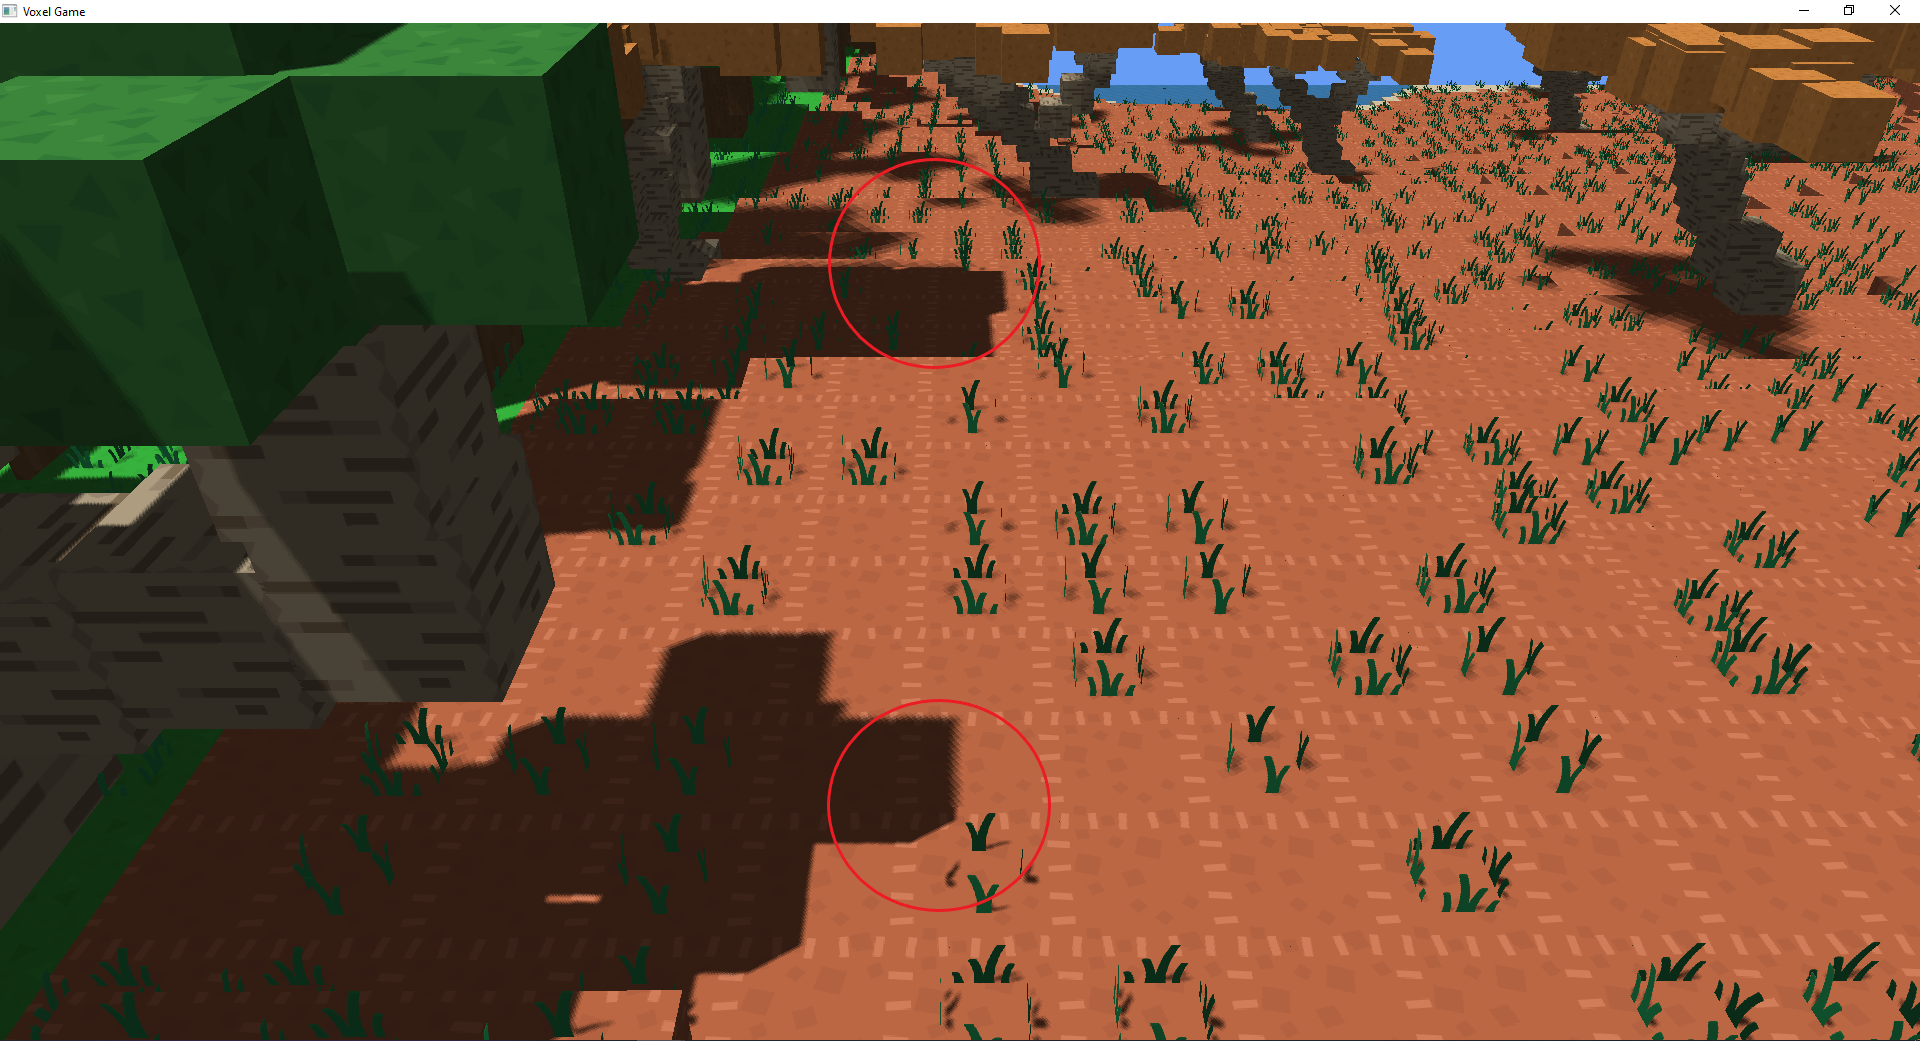
\includegraphics[width=\textwidth]{images/shadows/csm}
	\caption[Výsledek použití kaskádového mapování stínů]{Výsledek použití kaskádového mapování stínů}\label{fig:shadows_csm}
\end{figure}




% % % % % % % % % % % % % % % % % % % % % % % % % % % % 
% % Modelování rostlin s využitím L-systémů
% % % % % % % % % % % % % % % % % % % % % % % % % % % % 

\chapter{Modelování rostlin s využitím L-systémů}
Herní svět obsahuje velké množství vegetace a ač jsou si všechny stromy, keře typově podobné, hráč si velice rychle všimne, že jsou identické. Na obrázku~\ref{fig:identicke_stromy} vidíme tři druhy stromů, které jsou zkopírované po scéně. Stromy v levé zadní části mají různou výšku, přesto působí umělým dojmem.

Stromy v reálném světě jsou si podobné -- rozeznáváme jednotlivé druhy stromů, přesto neexistují dva stejné stromy. Pokud druh stromu zapíšeme formální gramatikou nazývanou L-systém, docílíme podobné struktury stromů, které se budou lišit v detailech.

\begin{figure}\centering
	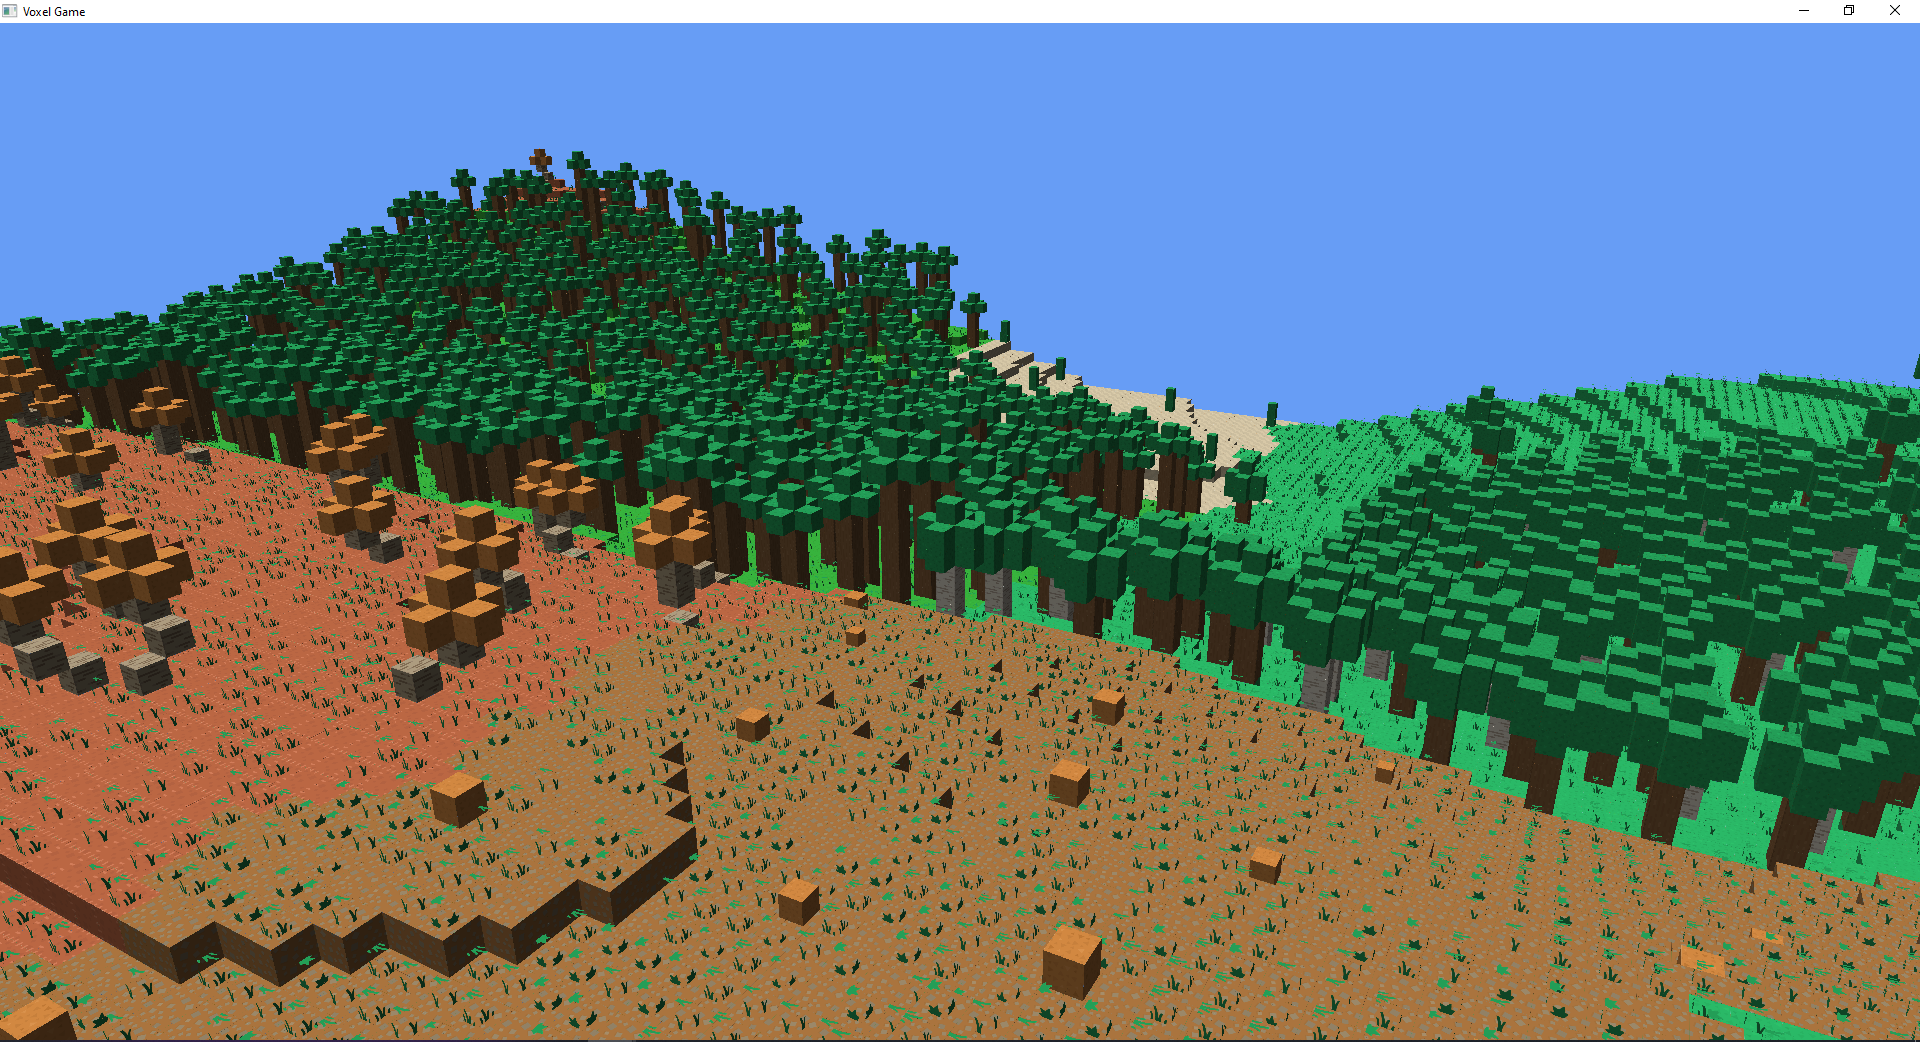
\includegraphics[width=\textwidth]{images/identical_trees}
	\caption[Identické stromy]{Identické stromy}\label{fig:identicke_stromy}
\end{figure}

\section{L-systém}
L-systém nebo také Lindenmayerův systém je paralelní přepisovací systém vyvinutý maďarským teoretickým biologem a botanistou Aristidem Lindenmayerem v roce 1968. L-systém je typ formální gramatiky skládající se z abecedy, přepisovacích pravidel a počátečního axiomu. Pomocí postupného derivování počátečního axiomu je možné simulovat vývoj rostliny v čase \cite{pcgbook75}.

\section{Interpretace řetězců pomocí želvy}
Řetězce lze graficky reprezentovat pomocí želvy, konzumující symboly abecedy. Každý symbol určuje akci, kterou má želva vykonat. Želva se může pohybovat ve 2D nebo 3D prostoru. Ve 2D si můžeme interpretaci představit jako želvu, držící tužku, pohybující se po papíře.

Želvu lze reprezentovat jako trojici $(x, y, \alpha)$, kde $(x, y)$ představuje kartézské souřadnice reprezentující polohu v prostoru a $\alpha$ úhel kam želva směřuje. Zadáním délky kroku \textit{d} a změny úhlu $\delta$ lze želvu ovládat pomocí následujících symbolů.

\begin{itemize}
\item F --- Posun dopředu o délku $d$. Stav želvy se změní na $(x’, y‘, \alpha)$, kde $x = x + d \cos \alpha$ a $y = y + d \sin \alpha$. Mezi body $(x, y)$ a $(x’, y‘)$ je nakreslena čára.
\item + --- Rotace doleva o úhel $\delta$. Nový stav želvy $(x, y, \alpha + \delta)$.
\item - --- Rotace doprava o úhel $\delta$. Nový stav želvy $(x, y, \alpha - \delta)$.
\end{itemize}

Nechť je definován následující L-systém. Buď $\omega$ počáteční axiom, $p$ přepisovací pravidlo, $\delta = 90\degree$ a $d$ zmenšené čtyřnásobně pro každý obrázek~\cite{abop7}.

\bigskip
$\omega: F-F-F-F$

\medskip
$p: F \rightarrow F-F+F+FF-F-F+F$

\bigskip
Želva interpretující daný L-systém generuje kvadratické Kochovy ostrovy~\ref{fig:koch_island}. Obrázky jsou vygenerovány derivacemi o délce 0 až 3.

\begin{figure}\centering
	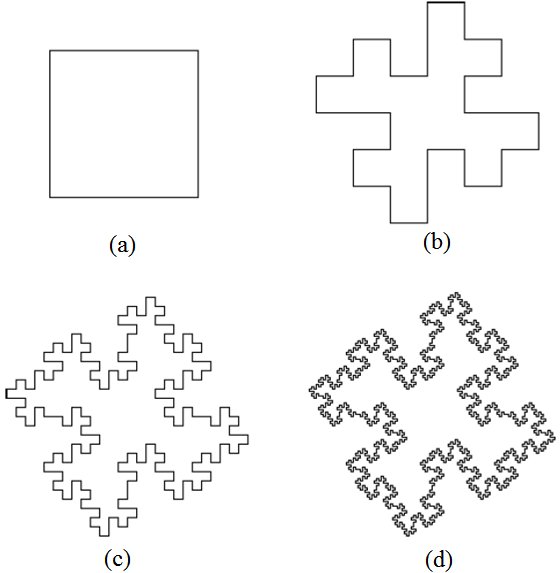
\includegraphics[width=\textwidth]{images/koch_island}
	\caption[Kvadratické Kochovy ostrovy]{Kvadratické Kochovy ostrovy}\label{fig:koch_island}
\end{figure}

\section{Větvení v L-systémech}
S danými přepisovacími pravidly není možné generovat větvící se struktury. Želva vždy pokračuje od své poslední pozice. Říše rostlin je dominovaná větvícími se strukturami, potřebujeme proto matematické vyjádření této skutečnosti.

Větvení v řetězci můžeme reprezentovat pomocí dvou symbolů [ a ], kde [ značí začátek větve a ] konec větve~\cite{abop24}.

Symboly jsou interpretovány želvou následovně:

\begin{itemize}
\item $[$ -- Ulož atributy želvy do zásobníku.
\item $]$ -- Načti atributy želvy ze zásobníku a smaž je z vrcholu zásobníku (operace pop). Při této operaci není nakreslená žádná čára.
\end{itemize}

Díky nově přidaným symbolům lze generovat struktury připomínající rostliny. Struktury na obrázku~\ref{fig:plant_like_str} jsou generované následujícími L-systémy:

\begin{enumerate}
\item $\delta = 20\degree$

	$\omega: E$
	
	$p1: F \rightarrow FF$
	
	$p2: E \rightarrow F[+E]F[-E]+E$
	
\item $\delta = 25,7\degree$

	$\omega: E$
	
	$p1: F \rightarrow FF$
	
	$p2: E \rightarrow F[+E][-E]FE$

\end{enumerate}

L-systém 1 generuje rostlinu vlevo, L-systém 2 generuje rostlinu vpravo.

\begin{figure}\centering
	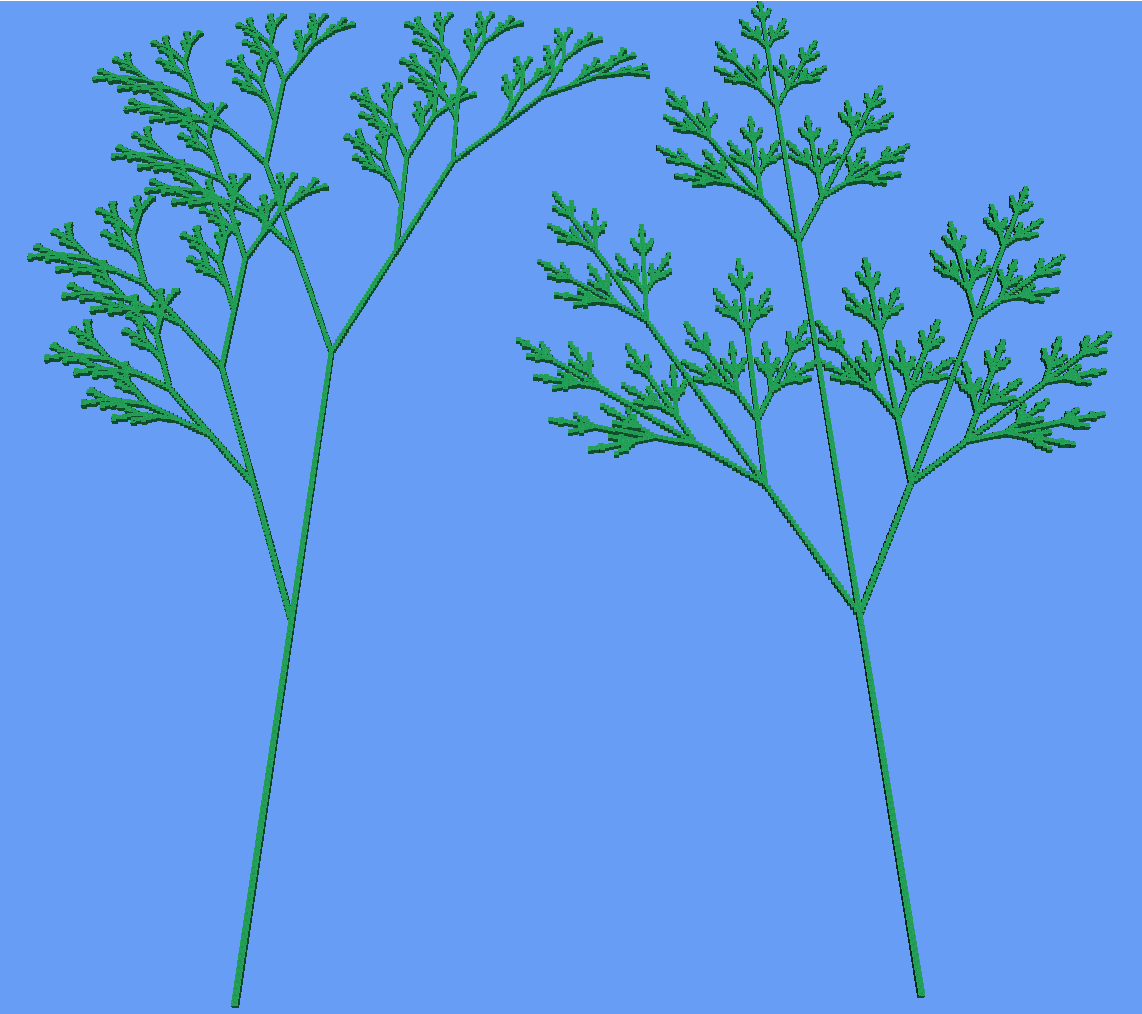
\includegraphics[width=\textwidth]{images/plant_d_e}
	\caption[Struktury připomínající rostliny]{Struktury připomínající rostliny generované pomocí závorkovaného systému}\label{fig:plant_like_str}
\end{figure}

\section{Stochastické L-systémy}
Rostliny generované deterministickým L-systémem jsou všechny stejné. Jejich použití ve scéně by vytvářelo stejný efekt, který je popsán na začátku kapitoly. 

K předejití tohoto efektu je nutné zavést variace v rámci druhu. Náhodná interpretace řetězce má limitované využití. Změna úhlu větvení, šířky a výšky segmentů rostliny zachovávají topologii struktury, ze které je generovaná. Stochastické L-systémy mohou měnit topologii struktury~\cite{abop28}.

L-systém, který byl do teď používán, nemohl mít více přepisovacích pravidel pro stejný symbol abecedy. Pokud má stochastický L-systém vice přepisovacích pravidel, je z nich vybráno jedno s pravděpodobností $1/n$, kde $n$ je počet přepisovacích pravidel pro daný symbol abecedy\footnote{Tato definice se liší, od definice uvedené ve~\cite{abop28}. Tento způsob náhodného výběru je použit v implementaci, kde pravděpodobnostní distribuci zastupuje několikanásobné zopakování přepisovacího pravidla.}.

Scéna~\ref{fig:plant_stoch} byla vygenerována za pomocí stochastického L-systému, kde:

\bigskip 
$\delta = 25,7\degree$

\medskip
$\omega: F$

\medskip
$p1: F \rightarrow F[+F]F[-F]F$

\medskip
$p2: F \rightarrow F[+F]F$

\medskip
$p3: F \rightarrow F[-F]F$

\begin{figure}\centering
	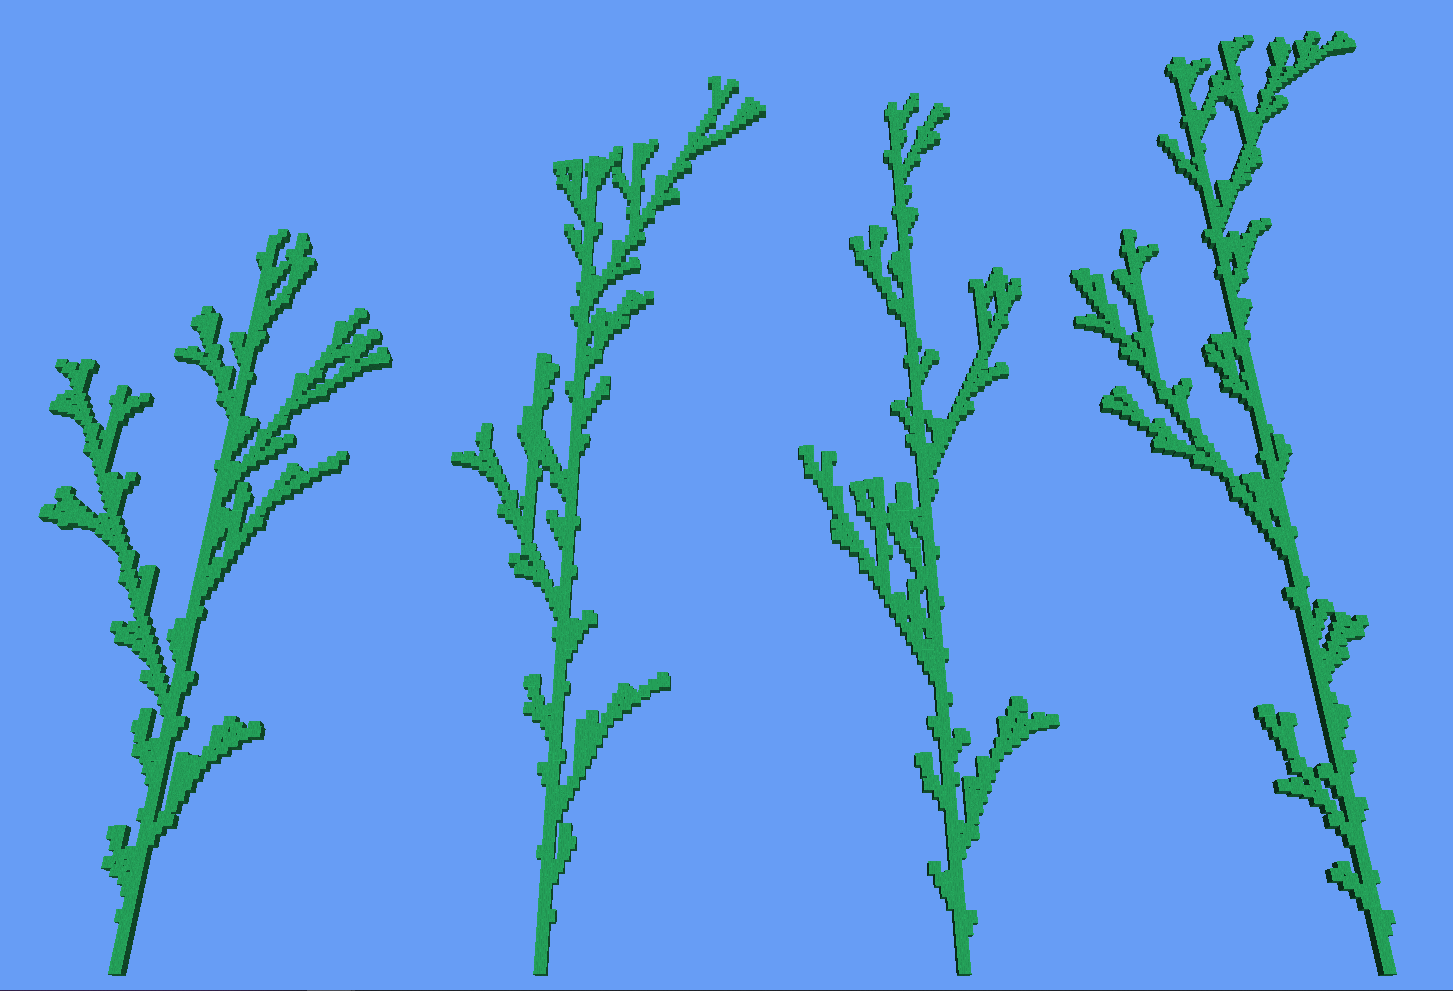
\includegraphics[width=\textwidth]{images/plant_stoch}
	\caption[Využití stochastického L-systému]{Využití stochastického L-systému}\label{fig:plant_stoch}
\end{figure}

\section{Implementace}
\subsection{Formát L-systému}

L-systém může být načten ze souboru pomocí třídy \texttt{LSystemParser}. L-systém musí mít následující formát:

\begin{verbatim}
yaw_angle pitch_angle shring_ratio
axiom
letter > production
.
.
.
letter > production
\end{verbatim}

Soubor může obsahovat za sebou jdoucí L-systémy. \texttt{LSystemParser} je vrátí jako pole. Soubor může obsahovat komentáře na nových řádcích, začínající symbolem \#.

Třída \texttt{LSystem} obsahuje gramatiku a tři atributy specifikující úhel náklonu podle osy y (yaw), podle osy x (pitch) a změnu velikosti bloku. Poslední atribut je využit při rozvětvení rostliny. Potomci mateřské větve by se měly řídit postulátem Leonarda da Vinci: „Všechny větve stromu, v každé úrovni jeho růstu, jsou v součtu jejich tloušťky rovné tloušťce kmene pod nimi.“ V případě dvojitého rozvětvení, tloušťky mateřské větve $w_1$, tloušťky potomků $w_2$ dostaneme rovnici~\cite{abop57}:

\[ w_1^2 = 2w_2^2 \]
\[ \frac{w_2}{w_1} = \frac{1}{\sqrt{2}} \approx 0,707\]

Hodnotu 0,7 je možné nalézt v L-systémech modelující keře.

\subsection{Želva}
Třída \texttt{Turtle} rozšiřuje pohyb želvy -- popsané v kapitole Interpretace řetězců pomocí želvy -- do 3D prostoru. Vnitřní stav želvy určují následující atributy:

\begin{itemize}
\item Pozice v prostoru.
\item Velikost bloku vytvořeného želvou.
\item Barva použitá pro kreslení (výstupní pole).
\item Yaw –- rotace podle osy y.
\item Pitch –- rotace podle osy x.
\end{itemize}

Želva si udržuje tři navzájem kolmé směrové vektory (nahoru, dopředu, doprava) jednotkové délky, které využívá pro pohyb po scéně. Vektory jsou aktualizované po každé rotaci. Pro výpočet je nutné znát vektor směřující kolmo vzhůru vůči scéně (\texttt{WORLD\_UP}). Generovaný svět je plochý, proto lze tento vektor nahradit konstantním vektorem $(0, 1, 0)$.

\begin{verbatim}
glm::vec3 front;
front.x = cos(glm::radians(Yaw_)) * cos(glm::radians(Pitch_));
front.y = sin(glm::radians(Pitch_));
front.z = sin(glm::radians(Yaw_)) * cos(glm::radians(Pitch_));

Front_ = glm::normalize(front);
Right_ = glm::normalize(glm::cross(Front_, WORLD_UP));
Up_ = glm::normalize(glm::cross(Right_, Front_));
\end{verbatim}

Délku \textit{x} v rovině určené osami \textit{x} a \textit{z} lze spočítat jako délku přilehlé odvěsny. $\cos(Yaw) = x / h$, kde \textit{h} je délka přepony. Víme, že vektor má jednotkovou délku, proto $h = 1$. Stejný postup aplikujeme pro rovinu určenou osami \textit{x} a \textit{y}.

Tímto způsobem dopočítáme délky \textit{y} a \textit{z} vektoru směřujícího dopředu a normalizujeme ho. Jelikož jsou na sebe vektory kolmé, využijeme vektorového součinu, jehož výsledkem je vektor kolmý k oběma původním vektorům. Všechny vektory je nutné normalizovat, aby se předešlo jejich zkracování s tím, jak se Pitch blíží $\pm 90\degree$.

K zamezení převrácení os jsou z definičního oboru Pitch vyjmuty násobky 90\degree.

\begin{verbatim}
if (Helpers::Math::Equal(cos(glm::radians(Pitch_)), 0.0f))
    Pitch_ -= 0.01f;
\end{verbatim}

Výsledná nepřesnost je menší než maximální rozdíl dvou čísle typu float~$\epsilon$, která jsou považována za stejná. Funkce \texttt{Equal} porovnává desetinná čísla s přesností~$\epsilon$.

Želva vystavuje metody pro pohyb ve všech třech osách využívající vektorů \texttt{Up\_, Right\_, Forward\_}. K pozici želvy je přičten patřičný vektor naškálovaný délkou pohybu. Např.:

\begin{verbatim}
void LSystems::Detail::Turtle::MoveForward(float dz) {
    Position_ += Front_ * dz;
}
\end{verbatim}

\subsection{Rozšířená abeceda}
Následující symboly abecedy mají speciální význam pro jejich interpretaci.

\begin{itemize}
\item U a u –- Posuň želvu nahoru.
\item F a f –- Posuň želvu dopředu.
\item x –- Zmenši blok produkovaný želvou.
\item X –- Zvětši blok produkovaný želvou.
\item S –- Nastav původní velikost bloku produkovaného želvou.
\item + –- Rotuj želvu doleva podle osy y.
\item - –- Rotuj želvu doprava podle osy y.
\item $\hat{}$ –- Rotuj želvu nahoru podle osy x.
\item \& –- Rotuj želvu dolů podle osy x.
\item $[$ –- Ulož kopii želvy na vrchol zásobníku.
\item $]$ –- Vyjmi želvu z vrcholu zásobníku.
\item $0-9$ –- Přepni výstupní pole.
\end{itemize}

L-systém může obsahovat jakýkoliv jiný ASCII symbol -- mimo bílých znaků a \# -- určený pro expanzi přepisovacích pravidel. Není želvou interpretován.

\subsection{Ovládání želvy}
Implementace želvy se nachází ve jmenném prostoru \texttt{LSystems::Detail}, uživatel by ji neměl využívat přímo, ale je pro něj připravena třída \texttt{LSystemExecutor} zajišťující generování herních objektů z poskytnutého L-systému.

\texttt{LSystemExecutor} umožňuje generovat herní objekty na základě stochastického L-systému -- topologie struktury výsledného modelu se může měnit mezi jednotlivými voláními generátoru na základě parametru \texttt{salt}. L-systém lze náhodně interpretovat na základě těchto parametrů:

\begin{itemize}
\item Rozsah počtu provedených derivací.
\item Variace v rotaci želvy. K úhlu, o který se má želva otočit, se přičte x * původní úhel, kde x je z [-angleVar, angleVar]. Defaultní hodnota angleVar je 0,2.
\item Výchozí velikost generovaných objektů. Lze určit rozsahem korespondujícím s počtem derivací.
\end{itemize}

Přidání náhodného úhlu má výrazný efekt na organický vzhled rostliny. Na obrázku~\ref{fig:acacia_random_angle_leaves} lze vidět akáciové stromy vyznačující se plochou korunou. V definici L-systému jsou všechny listy ve stejné výšce, výsledný rozdíl ve výškách je způsoben opakovaným rotováním želvy. V zápisu lze vidět, že se želva otočí o 45\degree nahoru (~$\hat{}$~), pokládá větve (u, U), skloní se o 45\degree (\&) a pokládá listy (F). Listy by tak měly být ve stejné rovině, ale nejsou.

L-systém generující akácie:

\begin{verbatim}
45.0 45.0 0.8
# make sure the plant has splits
# random lenght stem - then split
^uA1S&F+F+F+F
U > uU
A > +uuE
A > -uE
A > +uE
A > -E
A > uuE
A > uE
# top of the plant
E > x[++++UE1S&F+F+F+F]+UE
E > x[++++++UE1S&F+F+F+F]++UE
E > x[++UE1S&F+F+F+F]-UE
\end{verbatim}

\begin{figure}\centering
	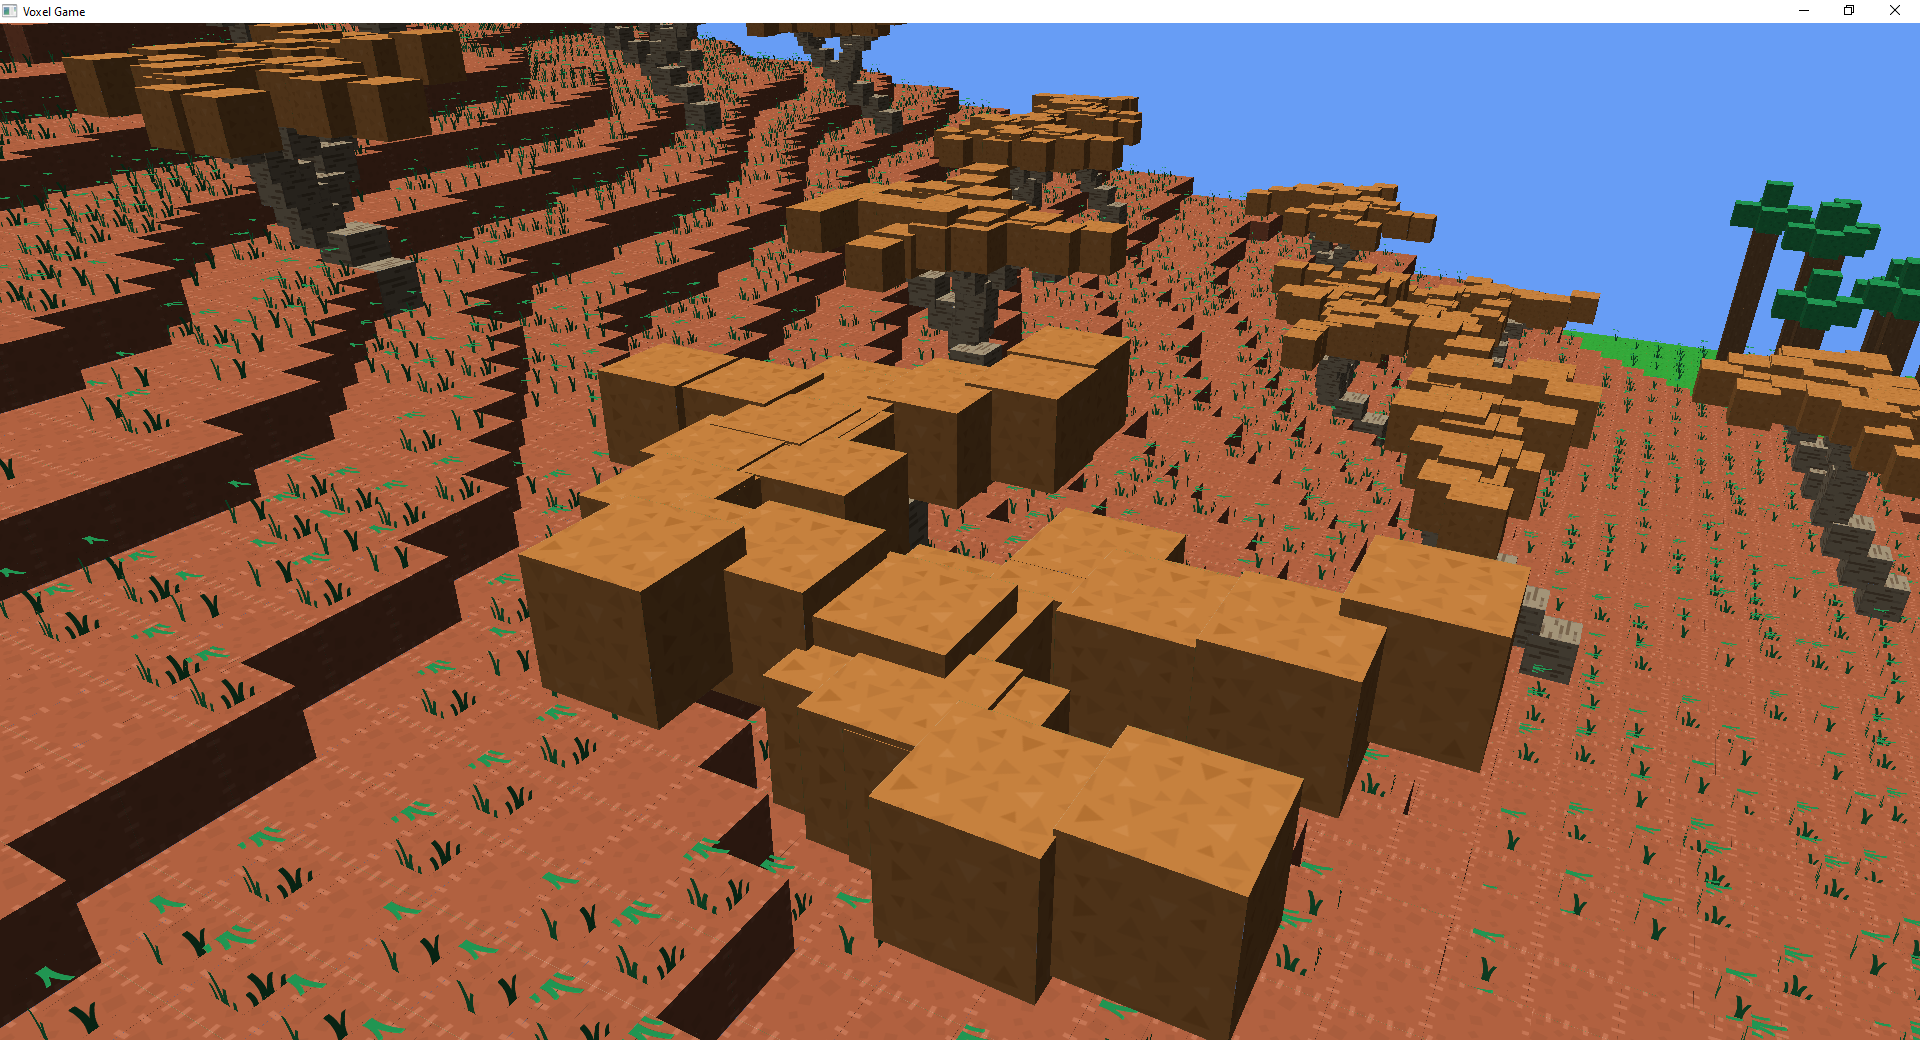
\includegraphics[width=\textwidth]{images/acacia_random_angle_leaves}
	\caption[Nepravidelná koruna akáciového stromu]{Nepravidelná koruna akáciového stromu}\label{fig:acacia_random_angle_leaves}
\end{figure}

Výstupem generátoru je 2D pole obsahující herní objekty rozdělené podle čísla výstupního bufferu, který měla želva při generování. Část enginu je tak odstíněna od textur, které jsou definované v~části procedurálního generátoru. Díky tomuto rozdělení modelu je možné snadno měnit textury pro jednotlivá pole. Procedurální generátor tohoto využívá a~používá stejný model -- jiný běh generátoru -- pro vytváření bříz a~dubů, lišících se texturou kmene a listů.

\section{Modelování rostlin}

Při modelování vegetace bylo třeba velkého množství pokusů a~ladění, kdy rostlina nevypadala přirozeně, ale nebylo jasné, v jaké časti gramatiky je problém. Nejvíce se mi osvědčila technika nalezení reálné rostliny obrázek~\ref{fig:acacia_nature} a~následné pokusy o její napodobení obrázek~\ref{fig:acacia_engine}.

Velice se osvědčilo pravidlo:

\begin{verbatim}
U > uU
\end{verbatim}

Díky němu jsou větve blíže k zemi delší, než větve navazující na korunu stromu. Pokud má rostlina význačné části je vhodné je modelovat samostatně (kmen, větve, koruna) viz L-systém generující akácie.

\begin{figure}\centering
	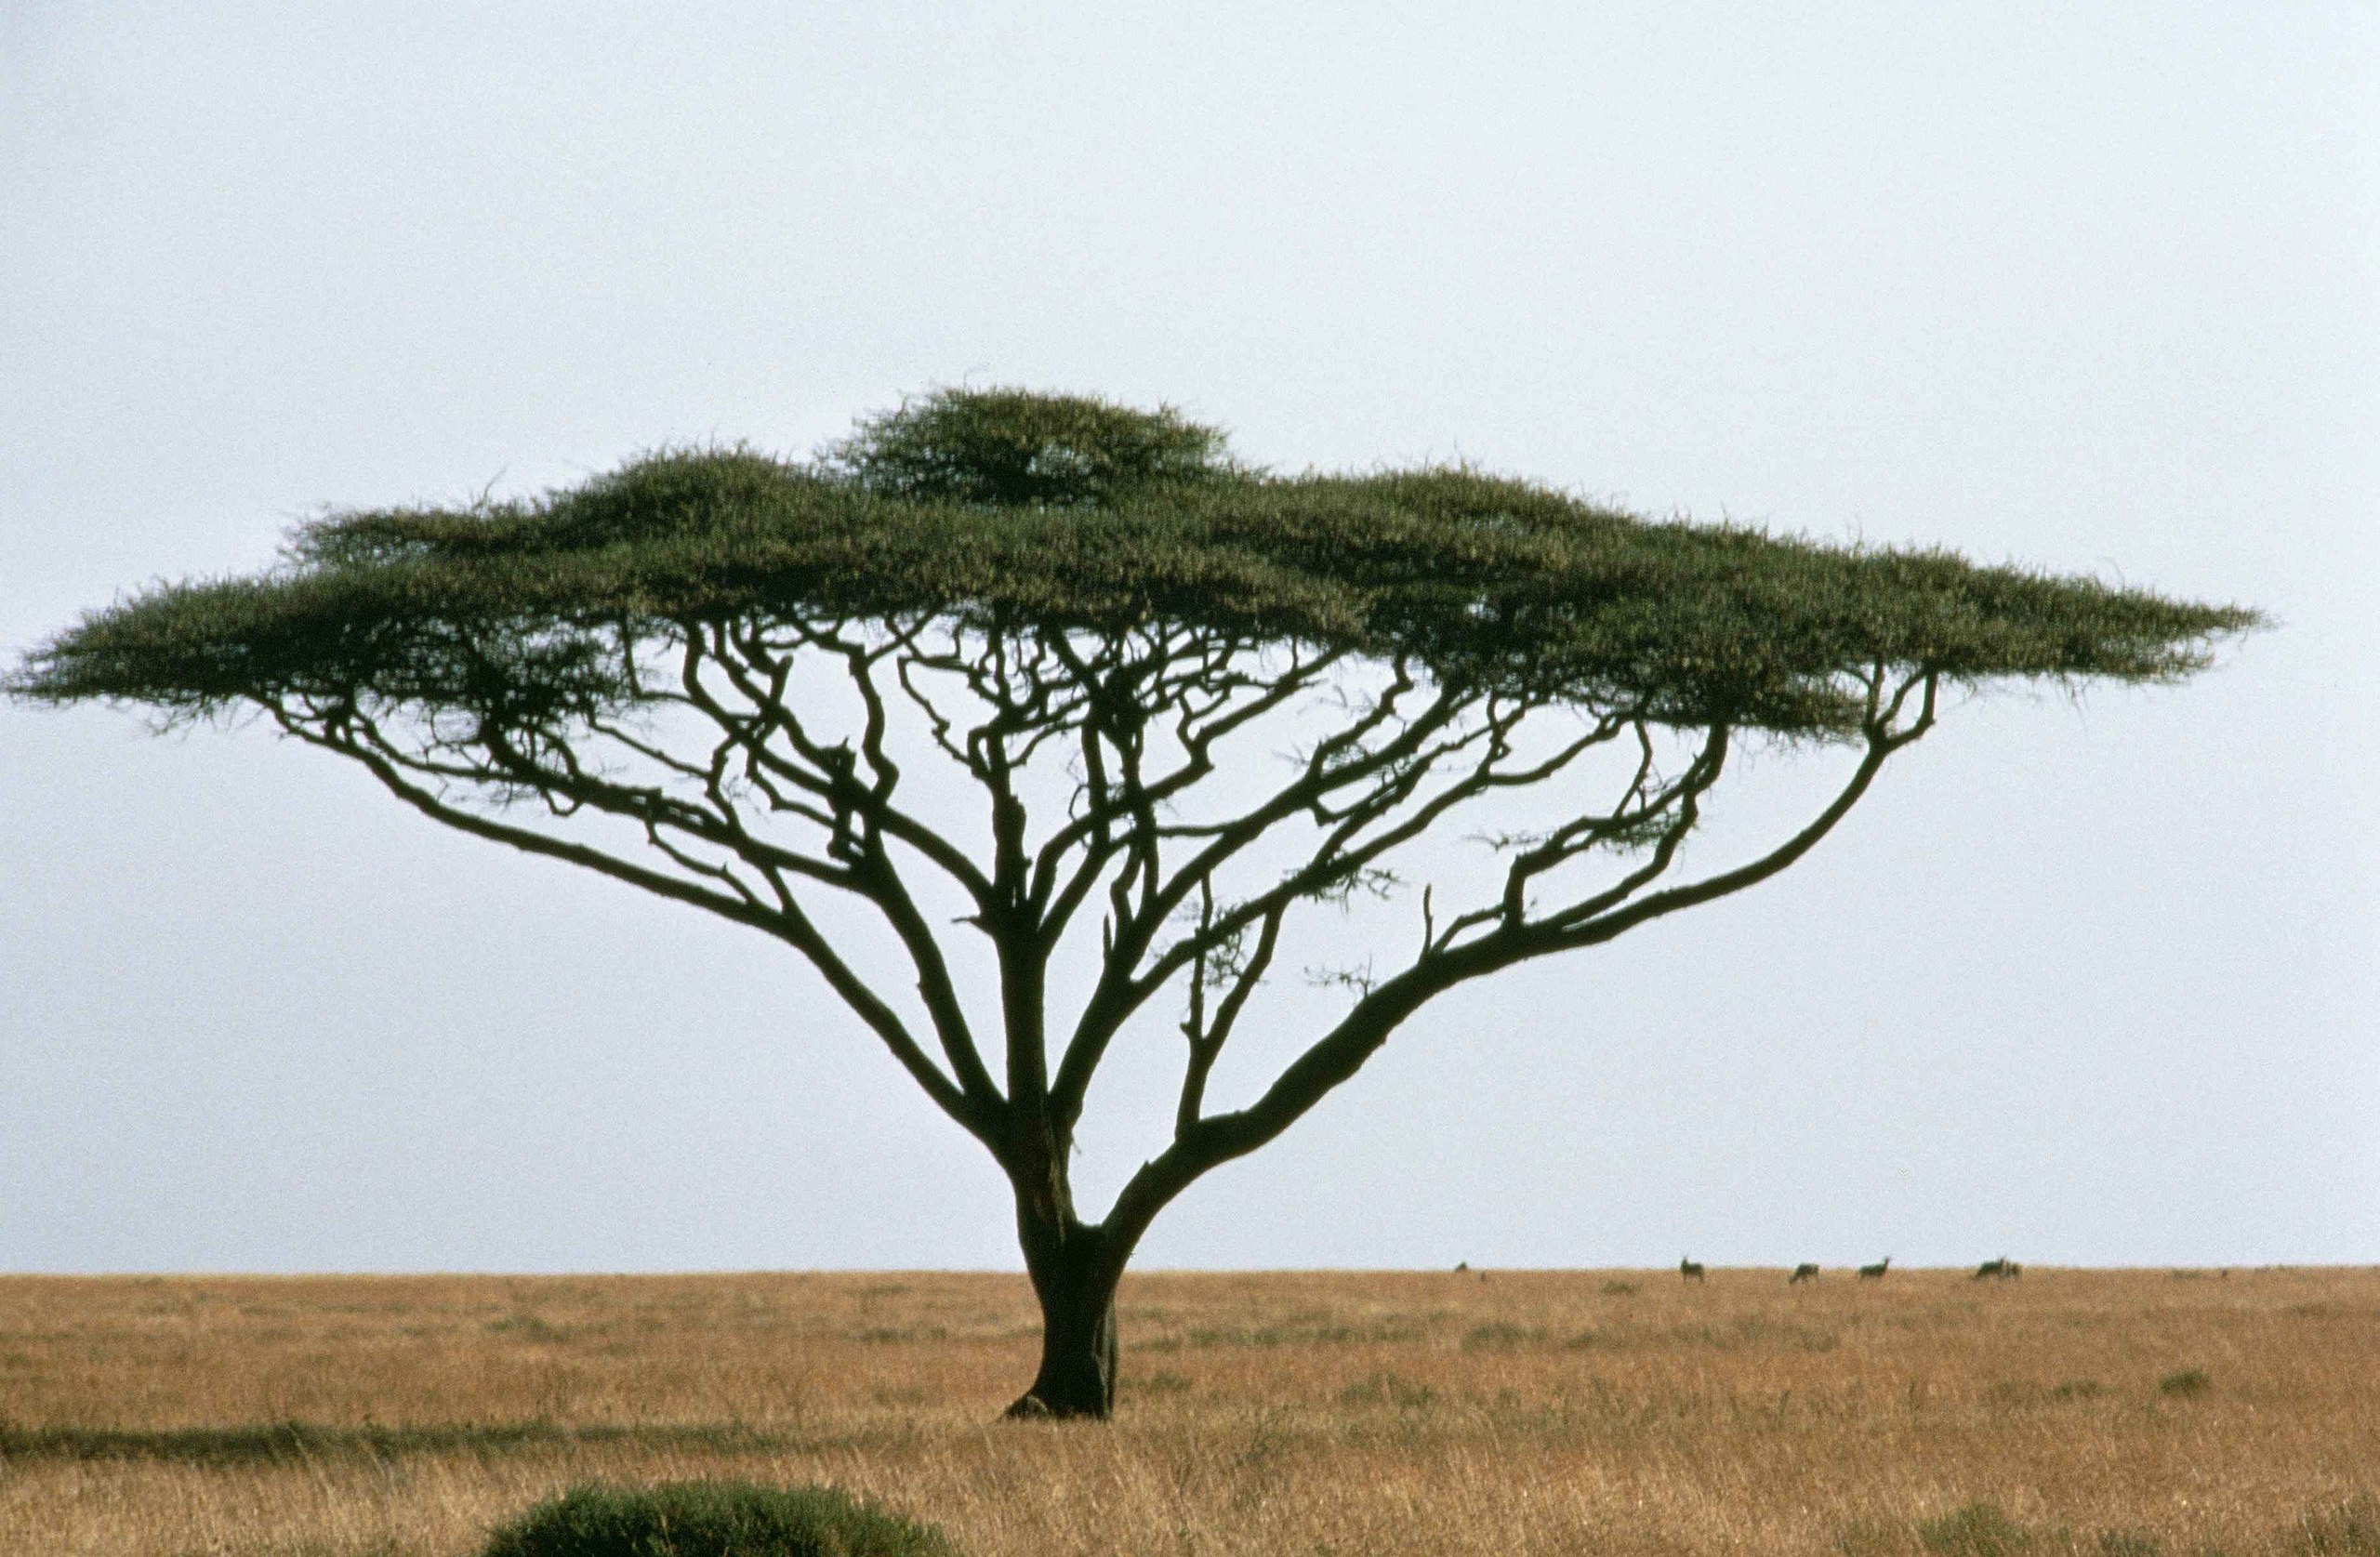
\includegraphics[width=\textwidth]{images/acacia_nature}
	\caption[Akáciový strom rostoucí v přírodě]{Akáciový strom rostoucí v přírodě~\cite{acacia}}\label{fig:acacia_nature}
\end{figure}

\begin{figure}\centering
	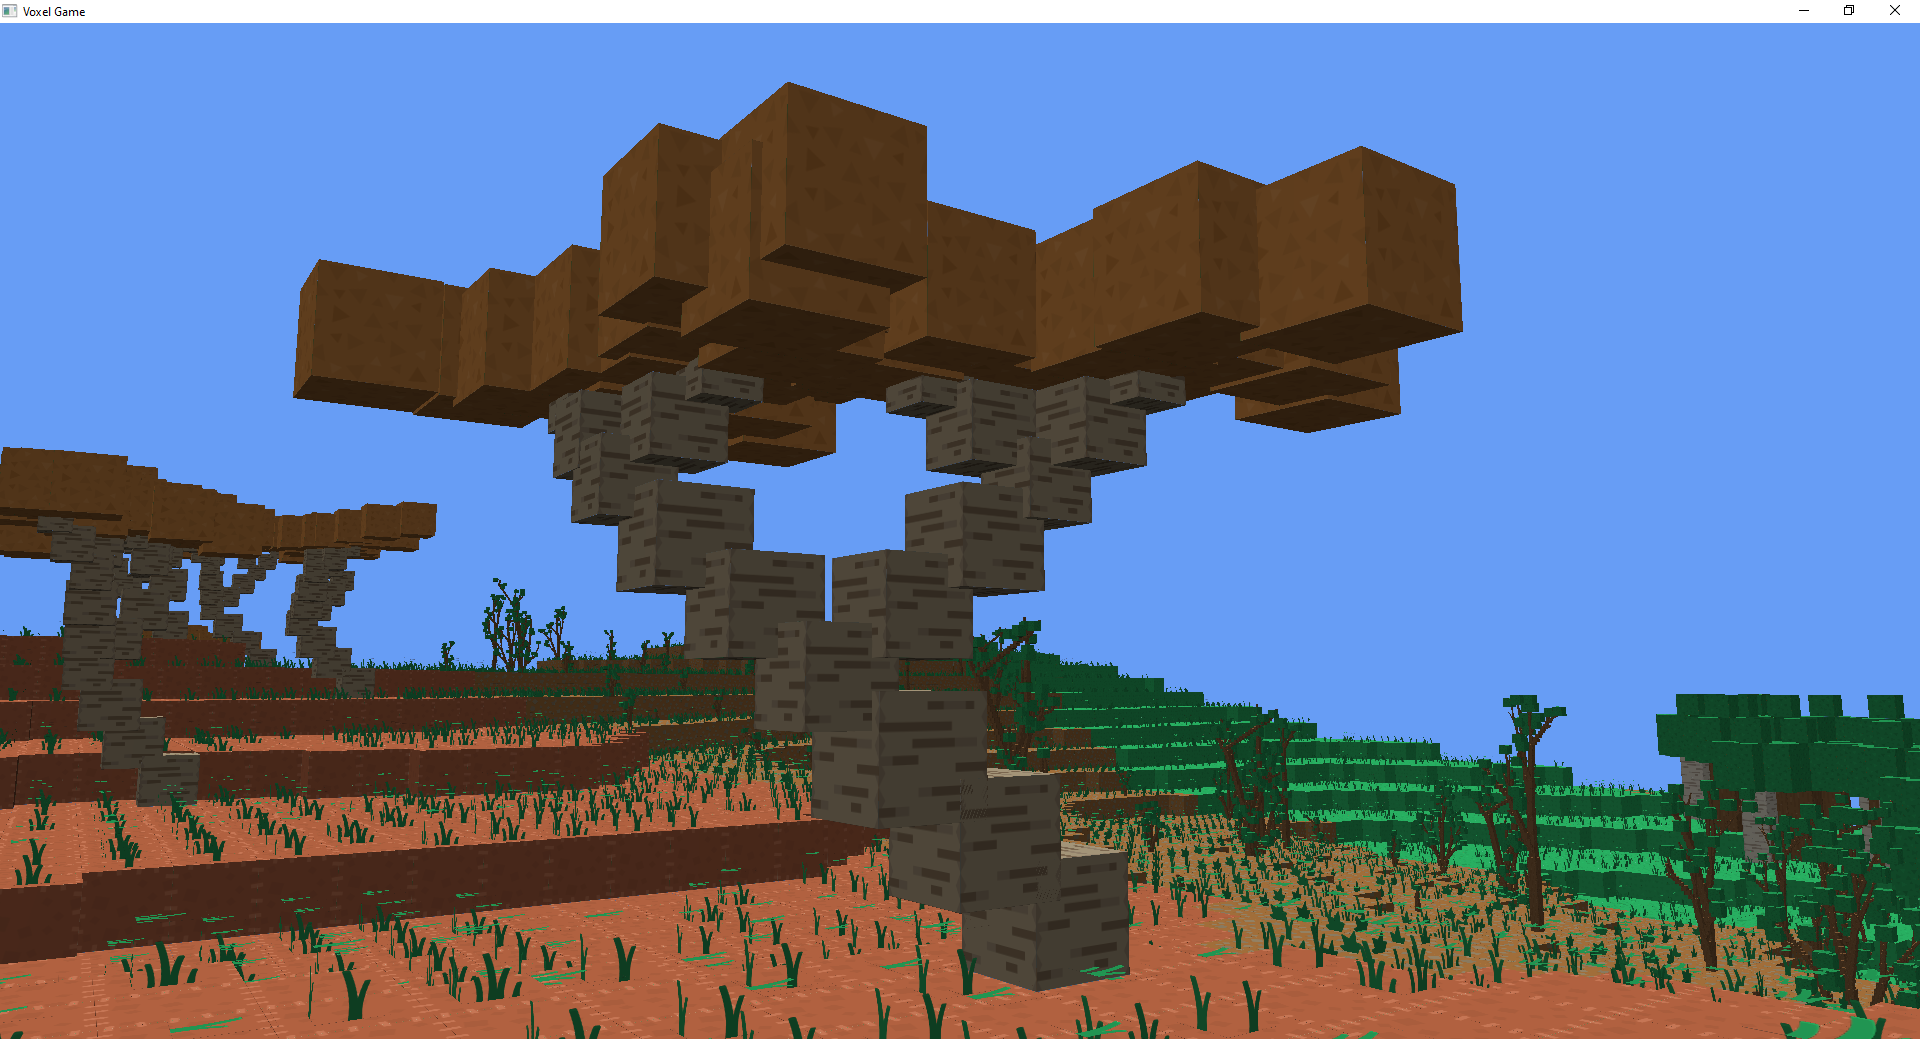
\includegraphics[width=\textwidth]{images/acacia_engine}
	\caption[Model akáciového stromu]{Model akáciového stromu}\label{fig:acacia_engine}
\end{figure}

Tato technika ne vždy přinášela ovoce. Modelování trávy rostoucí na planinách se projevilo jako problém. Tráva neměla dostatečnou hustotu a nezapadala do kresleného vzhledu -- obrázek~\ref{fig:grass_plains}. S navyšujícím se počtem herních objektů dramaticky rostla spotřeba paměti. Jeden herní objekt s texturou trávy byl nahrazen desítkami herních objektů, z kterých se skládal model trávy. Tento problém by mohl být řešen přesunem vytváření modelu na grafickou kartu, přidáním vertexů v geometry shaderu.

\begin{figure}\centering
	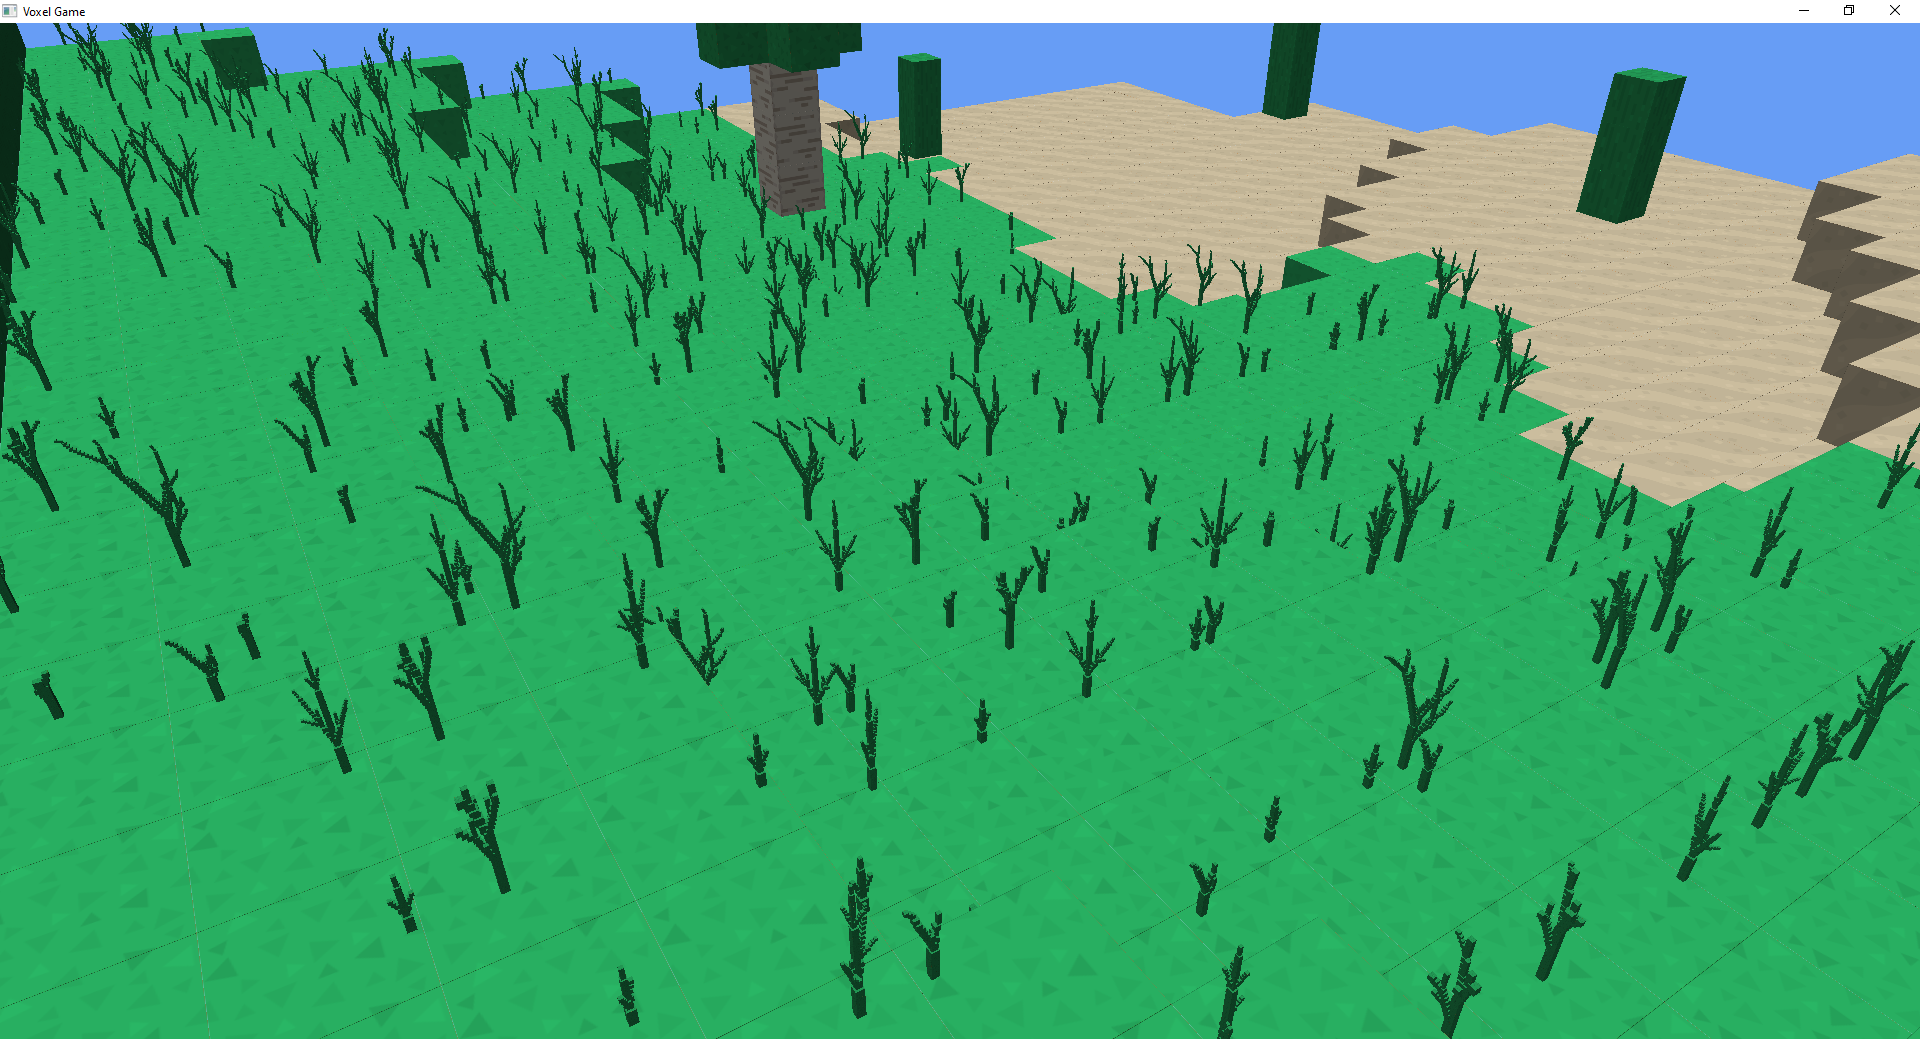
\includegraphics[width=\textwidth]{images/grass_plains}
	\caption[Tráva na planinách]{Tráva na planinách}\label{fig:grass_plains}
\end{figure}

Výsledné modely svou topologií připomínaly strukturu keřů. Byly proto upraveny -- přidáním listí, změnou větvení -- a využity v generátoru keřů.

\subsection{Simulace růstu}
Křovinatý biotop je porostlý dvěma druhy keřů, rozdělených do třech fází růstu. Ty jsou simulovány opakovaným derivováním počátečního axiomu. Keře nejmenšího vzrůstu jsou derivovány 2x, největší keře jsou derivovány 4x. Tloušťka kmene koreluje lineárně s počtem provedených derivací. Větší stromy mají širší kmen a dorůstají vyšší výšky.

Každý druh si zachovává své typické vlastnosti. Na obrázku~\ref{fig:shrub_evolution}\footnote{Pro větší názornost byly odstraněny části modelu představující listy.}  lze pozorovat stejné zakončení větví -- rozdělení do dvou větví rostoucích na opačné strany -- a~podobný úhel v~jakém se větve oddělují od kmene. Topologie rostliny se díky stochastickému L-systému mění mezi jednotlivými jedinci.

\begin{figure}\centering
	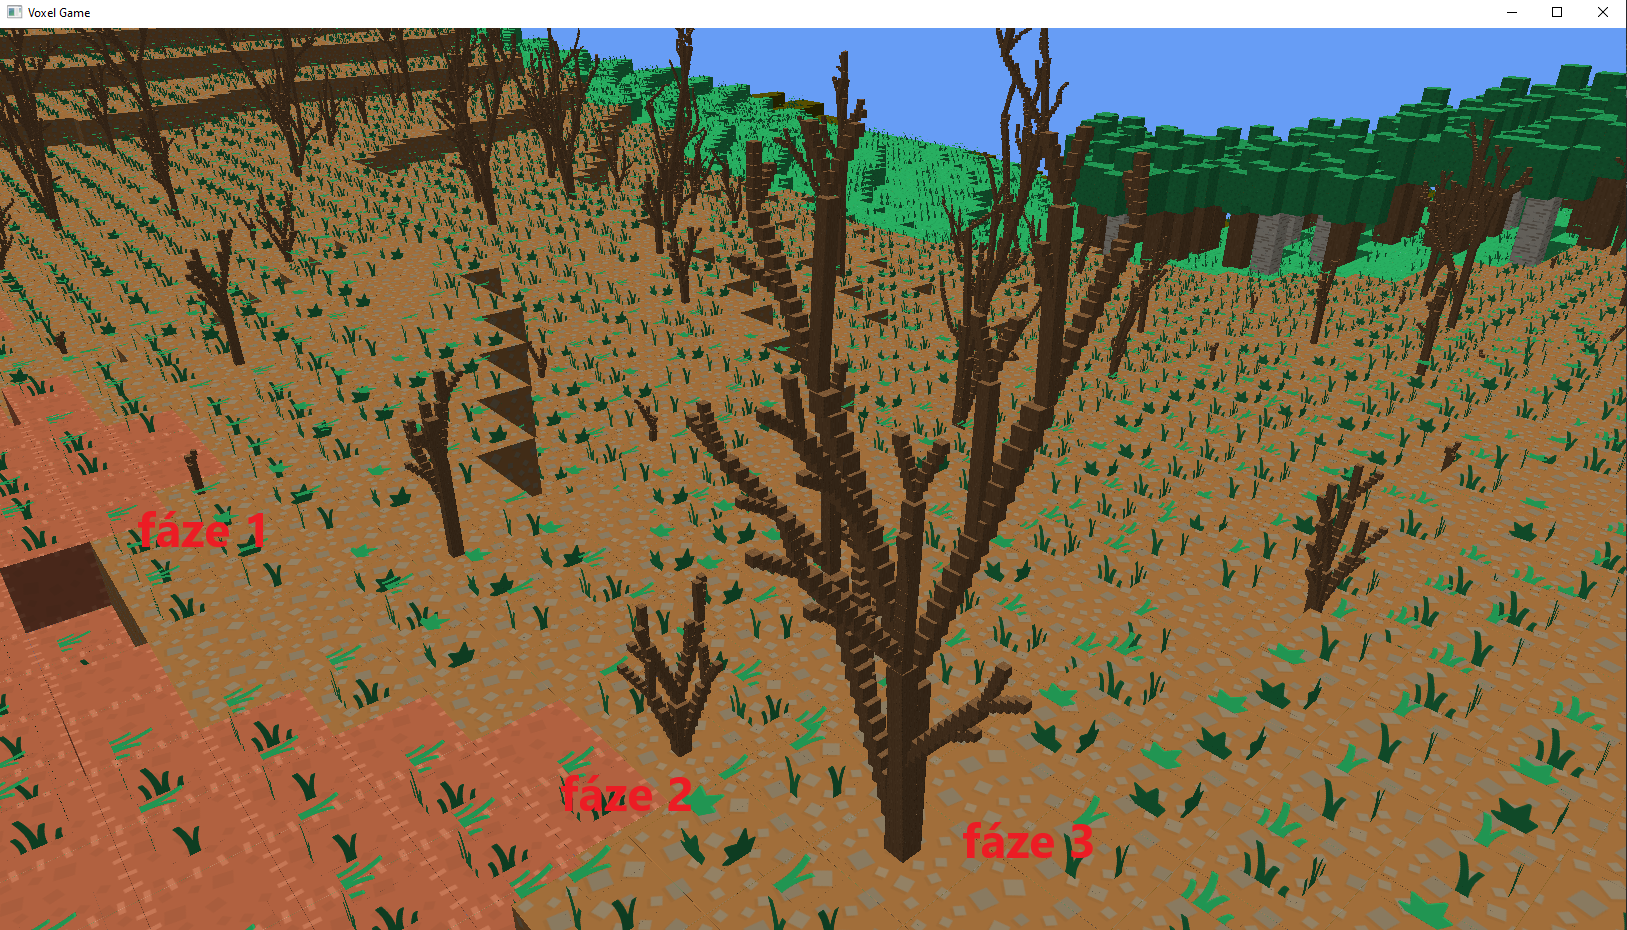
\includegraphics[width=\textwidth]{images/shrub_evolution}
	\caption[Fáze růstu keře]{Fáze růstu keře}\label{fig:shrub_evolution}
\end{figure}

Díky těmto krokům biotop obsahuje rostliny navzájem podobného vzhledu, lišících se v~drobných detailech.

\section{Výsledky použití L-systémů}
Definice L-systémů jsou krátké ($\approx$10 řádků na jeden druh rostliny) a produkují velké množství rozdílných jedinců. Předchozí manuální definování rostlin v kódu bylo náročnější, a i při přidání více jedinců pro každý druh, by bylo snadné najít stejné. Odebráním definic rostlin z kódu se zvýšila jeho čitelnost -- definice L-systémů jsou zdroje dat, který engine konzumuje. Nutnost kompilace při změně modelu byla odstraněna a zvýšila se rychlost iterace, s kterou je možné upravovat model.

Vytvořením vlastního formátu pro zápis modelu rostliny se oddělila závislost na programovacím jazyce. Modely tak může vytvářet jiný člen týmu bez znalosti programování a překladu kódu.

Generováním rostlin za běhu programu se snížila rychlost jeho běhu. Tento problém lze mitigovat cachováním rostlin obsahujících velké množství herních objektů. Toto bylo provedeno pro keře. Před spuštěním generace terénu je naplněn buffer obsahující keře vygenerované na základě seedu. Buffer musí být dostatečně velký na to, aby nedošlo ke snížení diverzity rostlin. Při vytváření keře na scéně je vybrán náhodný index do bufferu, závislý na pozici keře. Vybraný model je zkopírován a přesunut na dané místo.

Při porovnání scény~\ref{fig:identicke_stromy} ze začátku kapitoly si lze všimnout přirozenějšího vzhledu krajiny. Koruny stromů se mohou překrývat, scéna díky tomu působí více organicky -- stromy v přírodě nemají přesně stanové hranice, kde končí jeden a začíná druhý. Výsledná scenérie~\ref{fig:new_vegetation} působí méně jednolitě díky rozdílným vývojovým stádiím rostlin.

\begin{figure}\centering
	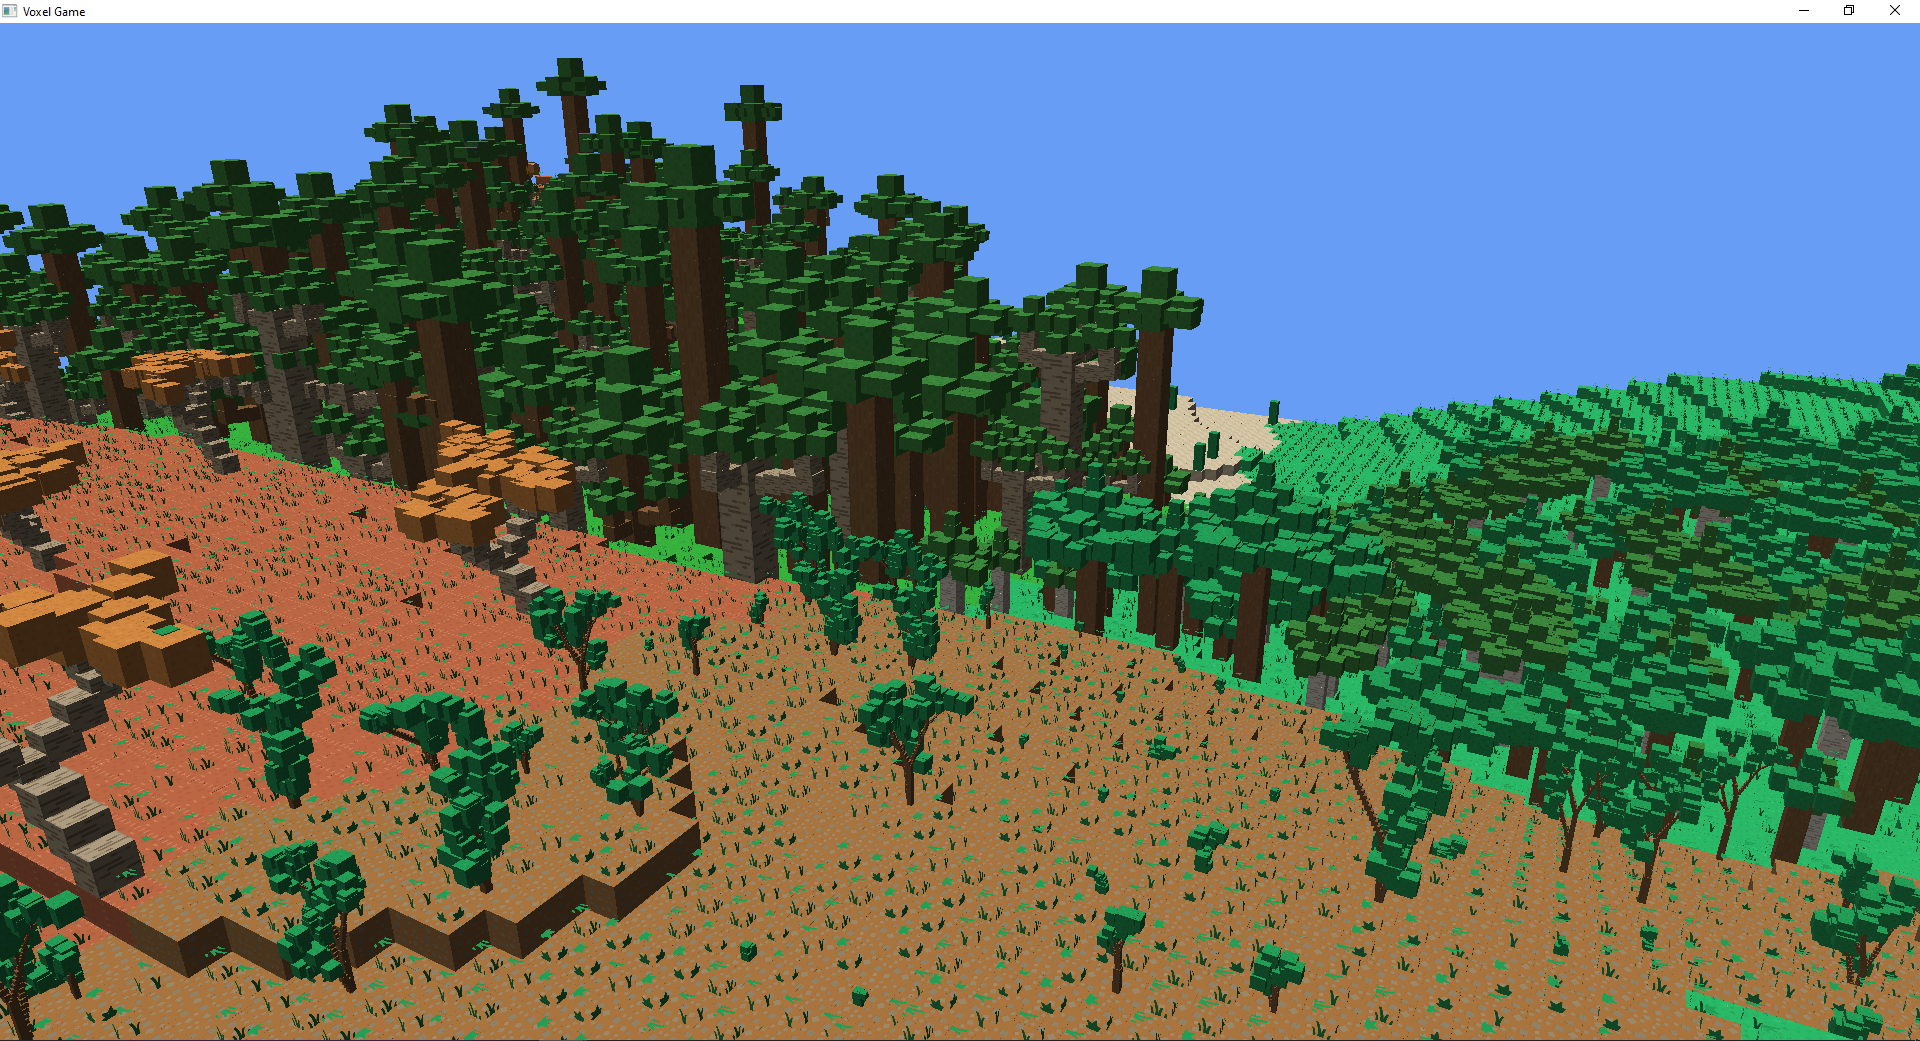
\includegraphics[width=\textwidth]{images/new_vegetation}
	\caption[Vegetace vygenerovaná na základě L-systémů]{Vegetace vygenerovaná na základě L-systémů}\label{fig:new_vegetation}
\end{figure}

% % % % % % % % % % % % % % % % % % % % % % % % % % % % 
% % ZAVER
% % % % % % % % % % % % % % % % % % % % % % % % % % % % 

\begin{conclusion}
	%sem napište závěr Vaší práce
\end{conclusion}

\bibliographystyle{csn690}
\bibliography{mybibliographyfile}

\appendix

\chapter{Seznam použitých zkratek}
% \printglossaries
\begin{description}
	\item[GUI] Graphical user interface
	\item[XML] Extensible markup language
\end{description}


% % % % % % % % % % % % % % % % % % % % % % % % % % % % 
% % Tuto kapitolu z výsledné práce ODSTRAŇTE.
% % % % % % % % % % % % % % % % % % % % % % % % % % % % 
% 
% \chapter{Návod k~použití této šablony}
% 
% Tento dokument slouží jako základ pro napsání závěrečné práce na Fakultě informačních technologií ČVUT v~Praze.
% 
% \section{Výběr základu}
% 
% Vyberte si šablonu podle druhu práce (bakalářská, diplomová), jazyka (čeština, angličtina) a kódování (ASCII, \mbox{UTF-8}, \mbox{ISO-8859-2} neboli latin2 a nebo \mbox{Windows-1250}). 
% 
% V~české variantě naleznete šablony v~souborech pojmenovaných ve formátu práce\_kódování.tex. Typ může být:
% \begin{description}
% 	\item[BP] bakalářská práce,
% 	\item[DP] diplomová (magisterská) práce.
% \end{description}
% Kódování, ve kterém chcete psát, může být:
% \begin{description}
% 	\item[UTF-8] kódování Unicode,
% 	\item[ISO-8859-2] latin2,
% 	\item[Windows-1250] znaková sada 1250 Windows.
% \end{description}
% V~případě nejistoty ohledně kódování doporučujeme následující postup:
% \begin{enumerate}
% 	\item Otevřete šablony pro kódování UTF-8 v~editoru prostého textu, který chcete pro psaní práce použít -- pokud můžete texty s~diakritikou normálně přečíst, použijte tuto šablonu.
% 	\item V~opačném případě postupujte dále podle toho, jaký operační systém používáte:
% 	\begin{itemize}
% 		\item v~případě Windows použijte šablonu pro kódování \mbox{Windows-1250},
% 		\item jinak zkuste použít šablonu pro kódování \mbox{ISO-8859-2}.
% 	\end{itemize}
% \end{enumerate}
% 
% 
% V~anglické variantě jsou šablony pojmenované podle typu práce, možnosti jsou:
% \begin{description}
% 	\item[bachelors] bakalářská práce,
% 	\item[masters] diplomová (magisterská) práce.
% \end{description}
% 
% \section{Použití šablony}
% 
% Šablona je určena pro zpracování systémem \LaTeXe{}. Text je možné psát v~textovém editoru jako prostý text, lze však také využít specializovaný editor pro \LaTeX{}, např. Kile.
% 
% Pro získání tisknutelného výstupu z~takto vytvořeného souboru použijte příkaz \verb|pdflatex|, kterému předáte cestu k~souboru jako parametr. Vhodný editor pro \LaTeX{} toto udělá za Vás. \verb|pdfcslatex| ani \verb|cslatex| \emph{nebudou} s~těmito šablonami fungovat.
% 
% Více informací o~použití systému \LaTeX{} najdete např. v~\cite{wikilatex}.
% 
% \subsection{Typografie}
% 
% Při psaní dodržujte typografické konvence zvoleného jazyka. České \uv{uvozovky} zapisujte použitím příkazu \verb|\uv|, kterému v~parametru předáte text, jenž má být v~uvozovkách. Anglické otevírací uvozovky se v~\LaTeX{}u zadávají jako dva zpětné apostrofy, uzavírací uvozovky jako dva apostrofy. Často chybně uváděný symbol "{} (palce) nemá s~uvozovkami nic společného.
% 
% Dále je třeba zabránit zalomení řádky mezi některými slovy, v~češtině např. za jednopísmennými předložkami a spojkami (vyjma \uv{a}). To docílíte vložením pružné nezalomitelné mezery -- znakem \texttt{\textasciitilde}. V~tomto případě to není třeba dělat ručně, lze použít program \verb|vlna|.
% 
% Více o~typografii viz \cite{kobltypo}.
% 
% \subsection{Obrázky}
% 
% Pro umožnění vkládání obrázků je vhodné použít balíček \verb|graphicx|, samotné vložení se provede příkazem \verb|\includegraphics|. Takto je možné vkládat obrázky ve formátu PDF, PNG a JPEG jestliže používáte pdf\LaTeX{} nebo ve formátu EPS jestliže používáte \LaTeX{}. Doporučujeme preferovat vektorové obrázky před rastrovými (vyjma fotografií).
% 
% \subsubsection{Získání vhodného formátu}
% 
% Pro získání vektorových formátů PDF nebo EPS z~jiných lze použít některý z~vektorových grafických editorů. Pro převod rastrového obrázku na vektorový lze použít rasterizaci, kterou mnohé editory zvládají (např. Inkscape). Pro konverze lze použít též nástroje pro dávkové zpracování běžně dodávané s~\LaTeX{}em, např. \verb|epstopdf|.
% 
% \subsubsection{Plovoucí prostředí}
% 
% Příkazem \verb|\includegraphics| lze obrázky vkládat přímo, doporučujeme však použít plovoucí prostředí, konkrétně \verb|figure|. Například obrázek \ref{fig:float} byl vložen tímto způsobem. Vůbec přitom nevadí, když je obrázek umístěn jinde, než bylo původně zamýšleno -- je tomu tak hlavně kvůli dodržení typografických konvencí. Namísto vynucování konkrétní pozice obrázku doporučujeme používat odkazování z~textu (dvojice příkazů \verb|\label| a \verb|\ref|).
% 
% \begin{figure}\centering
% 	
\includegraphics[width=0.5\textwidth, angle=30]{cvut-logo-bw}
% 	\caption[Příklad obrázku]{Ukázkový obrázek v~plovoucím prostředí}\label{fig:float}
% \end{figure}
% 
% \subsubsection{Verze obrázků}
% 
% % Gnuplot BW i barevně
% Může se hodit mít více verzí stejného obrázku, např. pro barevný či černobílý tisk a nebo pro prezentaci. S~pomocí některých nástrojů na generování grafiky je to snadné.
% 
% Máte-li například graf vytvořený v programu Gnuplot, můžete jeho černobílou variantu (viz obr. \ref{fig:gnuplot-bw}) vytvořit parametrem \verb|monochrome dashed| příkazu \verb|set term|. Barevnou variantu (viz obr. \ref{fig:gnuplot-col}) vhodnou na prezentace lze vytvořit parametrem \verb|colour solid|.
% 
% \begin{figure}\centering
% 	\includegraphics{gnuplot-bw}
% 	\caption{Černobílá varianta obrázku generovaného programem Gnuplot}\label{fig:gnuplot-bw}
% \end{figure}
% 
% \begin{figure}\centering
% 	\includegraphics{gnuplot-col}
% 	\caption{Barevná varianta obrázku generovaného programem Gnuplot}\label{fig:gnuplot-col}
% \end{figure}
% 
% 
% \subsection{Tabulky}
% 
% Tabulky lze zadávat různě, např. v~prostředí \verb|tabular|, avšak pro jejich vkládání platí to samé, co pro obrázky -- použijte plovoucí prostředí, v~tomto případě \verb|table|. Například tabulka \ref{tab:matematika} byla vložena tímto způsobem.
% 
% \begin{table}\centering
% 	\caption[Příklad tabulky]{Zadávání matematiky}\label{tab:matematika}
% 	\begin{tabular}{|l|l|c|c|}\hline
% 		Typ		& Prostředí		& \LaTeX{}ovská zkratka	& \TeX{}ovská zkratka	\tabularnewline \hline \hline
% 		Text		& \verb|math|		& \verb|\(...\)|	& \verb|$...$|		\tabularnewline \hline
% 		Displayed	& \verb|displaymath|	& \verb|\[...\]|	& \verb|$$...$$|	\tabularnewline \hline
% 	\end{tabular}
% \end{table}
% 
% % % % % % % % % % % % % % % % % % % % % % % % % % % % 

\chapter{Obsah přiloženého CD}

%upravte podle skutecnosti

\begin{figure}
	\dirtree{%
		.1 readme.txt\DTcomment{stručný popis obsahu CD}.
		.1 exe\DTcomment{adresář se spustitelnou formou implementace}.
		.1 src.
		.2 impl\DTcomment{zdrojové kódy implementace}.
		.2 thesis\DTcomment{zdrojová forma práce ve formátu \LaTeX{}}.
		.1 text\DTcomment{text práce}.
		.2 thesis.pdf\DTcomment{text práce ve formátu PDF}.
		.2 thesis.ps\DTcomment{text práce ve formátu PS}.
	}
\end{figure}

\end{document}
